% Plantilla para un Trabajo Fin de Grado de la Universidad de Granada,
% adaptada para el Doble Grado en Ingeniería Informática y Matemáticas.
%
%  Autor: Mario Román.
%  Licencia: GNU GPLv2.
%
% Esta plantilla es una adaptación al castellano de la plantilla
% classicthesis de André Miede, que puede obtenerse en:
%  https://ctan.org/tex-archive/macros/latex/contrib/classicthesis?lang=en
% La plantilla original se licencia en GNU GPLv2.
%
% Esta plantilla usa símbolos de la Universidad de Granada sujetos a la normativa
% de identidad visual corporativa, que puede encontrarse en:
% http://secretariageneral.ugr.es/pages/ivc/normativa
%
% La compilación se realiza con las siguientes instrucciones:
%   pdflatex --shell-escape main.tex
%   bibtex main
%   pdflatex --shell-escape main.tex
%   pdflatex --shell-escape main.tex

% Opciones del tipo de documento
\documentclass[twoside,openright,titlepage,numbers=noenddot,openany,headinclude,footinclude=true,
cleardoublepage=empty,abstractoff,BCOR=5mm,paper=a4,fontsize=12pt,main=spanish]{scrreprt}

% Paquetes de latex que se cargan al inicio. Cubren la entrada de
% texto, gráficos, código fuente y símbolofs.
\usepackage[utf8]{inputenc}
\usepackage[T1]{fontenc}
\usepackage{fixltx2e}
\usepackage{graphicx} % Inclusión de imágenes.
\usepackage{grffile}  % Distintos formatos para imágenes.
\usepackage{longtable} % Tablas multipágina.
\usepackage{wrapfig} % Coloca texto alrededor de una figura.
\usepackage{rotating}
\usepackage[normalem]{ulem}
\usepackage{amsmath}
\usepackage{dsfont}
\usepackage{textcomp}
\usepackage{amssymb}
\usepackage{capt-of}
\usepackage[colorlinks=true]{hyperref}
\usepackage{tikz} % Diagramas conmutativos.
\usepackage{minted} % Código fuente.
\usepackage[T1]{fontenc}
\usepackage[numbers]{natbib}

% PAQUETE MIO

\usepackage{float}

% Plantilla classicthesis
\usepackage[beramono,eulerchapternumbers,linedheaders,parts,a5paper,dottedtoc,
manychapters,pdfspacing]{classicthesis}

% Geometría y espaciado de párrafos.
\setcounter{secnumdepth}{0}
\usepackage{enumitem}
\setitemize{noitemsep,topsep=0pt,parsep=0pt,partopsep=0pt}
\setlist[enumerate]{topsep=0pt,itemsep=-1ex,partopsep=1ex,parsep=1ex}
\usepackage[top=1.1in, bottom=1.5in, left=1.4in, right=1.2in]{geometry}
\setlength\itemsep{0em}
\setlength{\parindent}{0pt}
\usepackage[skip=10pt]{parskip}

% Cosas tablas
\usepackage{tabularx}
\usepackage{colortbl}
\usepackage{array}
\newcolumntype{Y}{>{\centering\arraybackslash}X}
\definecolor{azulillo}{rgb}{0.68,0.85,0.9}

% Profundidad de la tabla de contenidos.
\setcounter{secnumdepth}{3}

% Usa el paquete minted para mostrar trozos de código.
% Pueden seleccionarse el lenguaje apropiado y el estilo del código.
\usepackage{minted}
\usemintedstyle{colorful}
\setminted{fontsize=\small}
\setminted[haskell]{linenos=false,fontsize=\small}
\renewcommand{\theFancyVerbLine}{\sffamily\textcolor[rgb]{0.5,0.5,1.0}{\oldstylenums{\arabic{FancyVerbLine}}}}

% Path para las imágenes
\graphicspath{{figures/}{diagramas/}}

% Archivos de configuración.
%------------------------
% Bibliotecas para matemáticas de latex
%------------------------
\usepackage{amsthm}
\usepackage{amsmath}
\usepackage{tikz}
\usepackage{tikz-cd}
\usetikzlibrary{shapes,fit}
\usepackage{bussproofs}
\EnableBpAbbreviations{}
\usepackage{mathtools}
\usepackage{scalerel}
\usepackage{stmaryrd}

%------------------------
% Estilos para los teoremas
%------------------------
\theoremstyle{plain}
\newtheorem{theorem}{Teorema}
\newtheorem{proposition}{Proposición}
\newtheorem{lemma}{Lema}
\newtheorem{corollary}{Corolario}

\theoremstyle{definition}
\newtheorem{definition}{Definición}
\newtheorem{postulate}{Postulado}
\newtheorem*{postulate 3'}{Postulate 3'}
\newtheorem*{postulate 2'}{Projective Measurement}


% Comento estas lineas originales intentando que diga dem
%\renewenvironment{proof}{{\bfseries Proof.}}{\qed}

% Change the proof style so it's in English and add \qed at the end.
%\renewenvironment{proof}{{\bfseries Proof.}}{\qed}

% Añadido por mi intentando que pone "Demostración" y no "Proof"
\renewenvironment{proof}{{\bfseries Demostración.}}{\qed}
\renewenvironment{proof}{{\bfseries Demostración.}}{\qed}
% hasta aqui

\theoremstyle{remark}
\newtheorem{remark}{Remark}
\newtheorem{exampleth}{Ejemplo}

\begingroup\makeatletter\@for\theoremstyle:=definition,remark,plain\do{\expandafter\g@addto@macro\csname th@\theoremstyle\endcsname{\addtolength\thm@preskip\parskip}}\endgroup

%------------------------
% Macros
% ------------------------

\newcommand*{\C}{\mathds{C}}
\newcommand*{\ra}{\rangle}
\newcommand*{\la}{\langle}

% Para poner sonrisa sobre puntos suspensivos. Uso: \overplace{n}{\dotsc}
\newcommand{\overplace}[2]{%
	\overset{\substack{#1\\\smile}}{#2}%
}  % En macros.tex se almacenan las opciones y comandos para escribir matemáticas.
% ****************************************************************************************************
% classicthesis-config.tex 
% formerly known as loadpackages.sty, classicthesis-ldpkg.sty, and classicthesis-preamble.sty 
% Use it at the beginning of your ClassicThesis.tex, or as a LaTeX Preamble 
% in your ClassicThesis.{tex,lyx} with % ****************************************************************************************************
% classicthesis-config.tex 
% formerly known as loadpackages.sty, classicthesis-ldpkg.sty, and classicthesis-preamble.sty 
% Use it at the beginning of your ClassicThesis.tex, or as a LaTeX Preamble 
% in your ClassicThesis.{tex,lyx} with % ****************************************************************************************************
% classicthesis-config.tex 
% formerly known as loadpackages.sty, classicthesis-ldpkg.sty, and classicthesis-preamble.sty 
% Use it at the beginning of your ClassicThesis.tex, or as a LaTeX Preamble 
% in your ClassicThesis.{tex,lyx} with \input{classicthesis-config}
% ****************************************************************************************************  
% If you like the classicthesis, then I would appreciate a postcard. 
% My address can be found in the file ClassicThesis.pdf. A collection 
% of the postcards I received so far is available online at 
% http://postcards.miede.de
% ****************************************************************************************************


% ****************************************************************************************************
% 0. Set the encoding of your files. UTF-8 is the only sensible encoding nowadays. If you can't read
% äöüßáéçèê∂åëæƒÏ€ then change the encoding setting in your editor, not the line below. If your editor
% does not support utf8 use another editor!
% ****************************************************************************************************
\PassOptionsToPackage{utf8x}{inputenc}
	\usepackage{inputenc}

% ****************************************************************************************************
% 1. Configure classicthesis for your needs here, e.g., remove "drafting" below 
% in order to deactivate the time-stamp on the pages
% ****************************************************************************************************
\PassOptionsToPackage{eulerchapternumbers,listings,drafting,%
		pdfspacing,%floatperchapter,%linedheaders,%
                subfig,beramono,eulermath,parts,dottedtoc}{classicthesis}                                        
% ********************************************************************
% Available options for classicthesis.sty 
% (see ClassicThesis.pdf for more information):
% drafting
% parts nochapters linedheaders
% eulerchapternumbers beramono eulermath pdfspacing minionprospacing
% tocaligned dottedtoc manychapters
% listings floatperchapter subfig
% ********************************************************************

% ****************************************************************************************************
% 2. Personal data and user ad-hoc commands
% ****************************************************************************************************
\newcommand{\myTitle}{TFG Ana Buendia\xspace}
\newcommand{\mySubtitle}{An Homage to The Elements of Typographic Style\xspace}
\newcommand{\myDegree}{Doktor-Ingenieur (Dr.-Ing.)\xspace}
\newcommand{\myName}{André Miede\xspace}
\newcommand{\myProf}{Put name here\xspace}
\newcommand{\myOtherProf}{Put name here\xspace}
\newcommand{\mySupervisor}{Put name here\xspace}
\newcommand{\myFaculty}{Put data here\xspace}
\newcommand{\myDepartment}{Put data here\xspace}
\newcommand{\myUni}{Put data here\xspace}
\newcommand{\myLocation}{Saarbrücken\xspace}
\newcommand{\myTime}{September 2015\xspace}
%\newcommand{\myVersion}{version 4.2\xspace}

% ********************************************************************
% Setup, finetuning, and useful commands
% ********************************************************************
\newcounter{dummy} % necessary for correct hyperlinks (to index, bib, etc.)
\newlength{\abcd} % for ab..z string length calculation
\providecommand{\mLyX}{L\kern-.1667em\lower.25em\hbox{Y}\kern-.125emX\@}
\newcommand{\ie}{i.\,e.}
\newcommand{\Ie}{I.\,e.}
\newcommand{\eg}{e.\,g.}
\newcommand{\Eg}{E.\,g.} 
% ****************************************************************************************************


% ****************************************************************************************************
% 3. Loading some handy packages
% ****************************************************************************************************
% ******************************************************************** 
% Packages with options that might require adjustments
% ******************************************************************** 
%\PassOptionsToPackage{ngerman,american}{babel}   % change this to your language(s)
% Spanish languages need extra options in order to work with this template
% \PassOptionsToPackage{es-lcroman,spanish}{babel}
\usepackage[main=spanish]{babel}

%\usepackage{csquotes}
% \PassOptionsToPackage{%
%     %backend=biber, %instead of bibtex
% 	backend=bibtex8,bibencoding=ascii,%
% 	language=auto,%
% 	style=alpha,%
%     %style=authoryear-comp, % Author 1999, 2010
%     %bibstyle=authoryear,dashed=false, % dashed: substitute rep. author with ---
%     sorting=nyt, % name, year, title
%     maxbibnames=10, % default: 3, et al.
%     %backref=true,%
%     natbib=true % natbib compatibility mode (\citep and \citet still work)
% }{biblatex}
%     \usepackage{biblatex}

% \PassOptionsToPackage{fleqn}{amsmath}       % math environments and more by the AMS 
%     \usepackage{amsmath}

% ******************************************************************** 
% General useful packages
% ******************************************************************** 
\PassOptionsToPackage{T1}{fontenc} % T2A for cyrillics
    \usepackage{fontenc}     
\usepackage{textcomp} % fix warning with missing font shapes
\usepackage{scrhack} % fix warnings when using KOMA with listings package          
\usepackage{xspace} % to get the spacing after macros right  
\usepackage{mparhack} % get marginpar right
\usepackage{fixltx2e} % fixes some LaTeX stuff --> since 2015 in the LaTeX kernel (see below)
%\usepackage[latest]{latexrelease} % will be used once available in more distributions (ISSUE #107)
\PassOptionsToPackage{printonlyused,smaller}{acronym} 
    \usepackage{acronym} % nice macros for handling all acronyms in the thesis
    %\renewcommand{\bflabel}[1]{{#1}\hfill} % fix the list of acronyms --> no longer working
    %\renewcommand*{\acsfont}[1]{\textsc{#1}} 
    \renewcommand*{\aclabelfont}[1]{\acsfont{#1}}
% ****************************************************************************************************


% ****************************************************************************************************
% 4. Setup floats: tables, (sub)figures, and captions
% ****************************************************************************************************
\usepackage{tabularx} % better tables
    \setlength{\extrarowheight}{3pt} % increase table row height
\newcommand{\tableheadline}[1]{\multicolumn{1}{c}{\spacedlowsmallcaps{#1}}}
\newcommand{\myfloatalign}{\centering} % to be used with each float for alignment
\usepackage{caption}
% Thanks to cgnieder and Claus Lahiri
% http://tex.stackexchange.com/questions/69349/spacedlowsmallcaps-in-caption-label
% [REMOVED DUE TO OTHER PROBLEMS, SEE ISSUE #82]    
%\DeclareCaptionLabelFormat{smallcaps}{\bothIfFirst{#1}{~}\MakeTextLowercase{\textsc{#2}}}
%\captionsetup{font=small,labelformat=smallcaps} % format=hang,
\captionsetup{font=small} % format=hang,
\usepackage{subfig}  
% ****************************************************************************************************


% ****************************************************************************************************
% 5. Setup code listings
% ****************************************************************************************************
% \usepackage{listings} 
% %\lstset{emph={trueIndex,root},emphstyle=\color{BlueViolet}}%\underbar} % for special keywords
% \lstset{language={Haskell},morekeywords={PassOptionsToPackage,selectlanguage},keywordstyle=\color{RoyalBlue},basicstyle=\small\ttfamily,commentstyle=\color{Green}\ttfamily,stringstyle=\rmfamily,numbers=none,numberstyle=\scriptsize,stepnumber=5,numbersep=8pt,showstringspaces=false,breaklines=true,belowcaptionskip=.75\baselineskip} 
% ****************************************************************************************************             


% ****************************************************************************************************
% 6. PDFLaTeX, hyperreferences and citation backreferences
% ****************************************************************************************************
% ********************************************************************
% Using PDFLaTeX
% ********************************************************************
\PassOptionsToPackage{pdftex,hyperfootnotes=false,pdfpagelabels}{hyperref}
    \usepackage{hyperref}  % backref linktocpage pagebackref
\pdfcompresslevel=9
\pdfadjustspacing=1 
\PassOptionsToPackage{pdftex}{graphicx}
    \usepackage{graphicx} 
 

% ********************************************************************
% Hyperreferences
% ********************************************************************
\hypersetup{%
    %draft, % = no hyperlinking at all (useful in b/w printouts)
    colorlinks=true, linktocpage=true, pdfstartpage=3, pdfstartview=FitV,%
    % uncomment the following line if you want to have black links (e.g., for printing)
    %colorlinks=false, linktocpage=false, pdfstartpage=3, pdfstartview=FitV, pdfborder={0 0 0},%
    breaklinks=true, pdfpagemode=UseNone, pageanchor=true, pdfpagemode=UseOutlines,%
    plainpages=false, bookmarksnumbered, bookmarksopen=true, bookmarksopenlevel=1,%
    hypertexnames=true, pdfhighlight=/O,%nesting=true,%frenchlinks,%
    urlcolor=webbrown, linkcolor=RoyalBlue, citecolor=webgreen, %pagecolor=RoyalBlue,%
    %urlcolor=Black, linkcolor=Black, citecolor=Black, %pagecolor=Black,%
    pdftitle={\myTitle},%
    pdfauthor={\textcopyright\ \myName, \myUni, \myFaculty},%
    pdfsubject={},%
    pdfkeywords={},%
    pdfcreator={pdfLaTeX},%
    pdfproducer={LaTeX with hyperref and classicthesis}%
}   

% ********************************************************************
% Setup autoreferences
% ********************************************************************
% There are some issues regarding autorefnames
% http://www.ureader.de/msg/136221647.aspx
% http://www.tex.ac.uk/cgi-bin/texfaq2html?label=latexwords
% you have to redefine the makros for the 
% language you use, e.g., american, ngerman
% (as chosen when loading babel/AtBeginDocument)
% ********************************************************************
\makeatletter
\@ifpackageloaded{babel}%
    {%
       \addto\extrasamerican{%
			\renewcommand*{\figureautorefname}{Figure}%
			\renewcommand*{\tableautorefname}{Table}%
			\renewcommand*{\partautorefname}{Part}%
			\renewcommand*{\chapterautorefname}{Chapter}%
			\renewcommand*{\sectionautorefname}{Section}%
			\renewcommand*{\subsectionautorefname}{Section}%
			\renewcommand*{\subsubsectionautorefname}{Section}%     
                }%
       \addto\extrasngerman{% 
			\renewcommand*{\paragraphautorefname}{Absatz}%
			\renewcommand*{\subparagraphautorefname}{Unterabsatz}%
			\renewcommand*{\footnoteautorefname}{Fu\"snote}%
			\renewcommand*{\FancyVerbLineautorefname}{Zeile}%
			\renewcommand*{\theoremautorefname}{Theorem}%
			\renewcommand*{\appendixautorefname}{Anhang}%
			\renewcommand*{\equationautorefname}{Gleichung}%        
			\renewcommand*{\itemautorefname}{Punkt}%
                }%  
            % Fix to getting autorefs for subfigures right (thanks to Belinda Vogt for changing the definition)
            \providecommand{\subfigureautorefname}{\figureautorefname}%             
    }{\relax}
\makeatother


% ****************************************************************************************************
% 7. Last calls before the bar closes
% ****************************************************************************************************
% ********************************************************************
% Development Stuff
% ********************************************************************
\listfiles
%\PassOptionsToPackage{l2tabu,orthodox,abort}{nag}
%   \usepackage{nag}
%\PassOptionsToPackage{warning, all}{onlyamsmath}
%   \usepackage{onlyamsmath}

% ********************************************************************
% Last, but not least...
% ********************************************************************
\usepackage{classicthesis} 
% ****************************************************************************************************


% ****************************************************************************************************
% 8. Further adjustments (experimental)
% ****************************************************************************************************
% ********************************************************************
% Changing the text area
% ********************************************************************
%\linespread{1.05} % a bit more for Palatino
%\areaset[current]{312pt}{761pt} % 686 (factor 2.2) + 33 head + 42 head \the\footskip
%\setlength{\marginparwidth}{7em}%
%\setlength{\marginparsep}{2em}%

% ********************************************************************
% Using different fonts
% ********************************************************************
%\usepackage[oldstylenums]{kpfonts} % oldstyle notextcomp
%\usepackage[osf]{libertine}
%\usepackage[light,condensed,math]{iwona}
%\renewcommand{\sfdefault}{iwona}
%\usepackage{lmodern} % <-- no osf support :-(
%\usepackage{cfr-lm} % 
%\usepackage[urw-garamond]{mathdesign} <-- no osf support :-(
%\usepackage[default,osfigures]{opensans} % scale=0.95 
%\usepackage[sfdefault]{FiraSans}
% ****************************************************************************************************

% ****************************************************************************************************  
% If you like the classicthesis, then I would appreciate a postcard. 
% My address can be found in the file ClassicThesis.pdf. A collection 
% of the postcards I received so far is available online at 
% http://postcards.miede.de
% ****************************************************************************************************


% ****************************************************************************************************
% 0. Set the encoding of your files. UTF-8 is the only sensible encoding nowadays. If you can't read
% äöüßáéçèê∂åëæƒÏ€ then change the encoding setting in your editor, not the line below. If your editor
% does not support utf8 use another editor!
% ****************************************************************************************************
\PassOptionsToPackage{utf8x}{inputenc}
	\usepackage{inputenc}

% ****************************************************************************************************
% 1. Configure classicthesis for your needs here, e.g., remove "drafting" below 
% in order to deactivate the time-stamp on the pages
% ****************************************************************************************************
\PassOptionsToPackage{eulerchapternumbers,listings,drafting,%
		pdfspacing,%floatperchapter,%linedheaders,%
                subfig,beramono,eulermath,parts,dottedtoc}{classicthesis}                                        
% ********************************************************************
% Available options for classicthesis.sty 
% (see ClassicThesis.pdf for more information):
% drafting
% parts nochapters linedheaders
% eulerchapternumbers beramono eulermath pdfspacing minionprospacing
% tocaligned dottedtoc manychapters
% listings floatperchapter subfig
% ********************************************************************

% ****************************************************************************************************
% 2. Personal data and user ad-hoc commands
% ****************************************************************************************************
\newcommand{\myTitle}{TFG Ana Buendia\xspace}
\newcommand{\mySubtitle}{An Homage to The Elements of Typographic Style\xspace}
\newcommand{\myDegree}{Doktor-Ingenieur (Dr.-Ing.)\xspace}
\newcommand{\myName}{André Miede\xspace}
\newcommand{\myProf}{Put name here\xspace}
\newcommand{\myOtherProf}{Put name here\xspace}
\newcommand{\mySupervisor}{Put name here\xspace}
\newcommand{\myFaculty}{Put data here\xspace}
\newcommand{\myDepartment}{Put data here\xspace}
\newcommand{\myUni}{Put data here\xspace}
\newcommand{\myLocation}{Saarbrücken\xspace}
\newcommand{\myTime}{September 2015\xspace}
%\newcommand{\myVersion}{version 4.2\xspace}

% ********************************************************************
% Setup, finetuning, and useful commands
% ********************************************************************
\newcounter{dummy} % necessary for correct hyperlinks (to index, bib, etc.)
\newlength{\abcd} % for ab..z string length calculation
\providecommand{\mLyX}{L\kern-.1667em\lower.25em\hbox{Y}\kern-.125emX\@}
\newcommand{\ie}{i.\,e.}
\newcommand{\Ie}{I.\,e.}
\newcommand{\eg}{e.\,g.}
\newcommand{\Eg}{E.\,g.} 
% ****************************************************************************************************


% ****************************************************************************************************
% 3. Loading some handy packages
% ****************************************************************************************************
% ******************************************************************** 
% Packages with options that might require adjustments
% ******************************************************************** 
%\PassOptionsToPackage{ngerman,american}{babel}   % change this to your language(s)
% Spanish languages need extra options in order to work with this template
% \PassOptionsToPackage{es-lcroman,spanish}{babel}
\usepackage[main=spanish]{babel}

%\usepackage{csquotes}
% \PassOptionsToPackage{%
%     %backend=biber, %instead of bibtex
% 	backend=bibtex8,bibencoding=ascii,%
% 	language=auto,%
% 	style=alpha,%
%     %style=authoryear-comp, % Author 1999, 2010
%     %bibstyle=authoryear,dashed=false, % dashed: substitute rep. author with ---
%     sorting=nyt, % name, year, title
%     maxbibnames=10, % default: 3, et al.
%     %backref=true,%
%     natbib=true % natbib compatibility mode (\citep and \citet still work)
% }{biblatex}
%     \usepackage{biblatex}

% \PassOptionsToPackage{fleqn}{amsmath}       % math environments and more by the AMS 
%     \usepackage{amsmath}

% ******************************************************************** 
% General useful packages
% ******************************************************************** 
\PassOptionsToPackage{T1}{fontenc} % T2A for cyrillics
    \usepackage{fontenc}     
\usepackage{textcomp} % fix warning with missing font shapes
\usepackage{scrhack} % fix warnings when using KOMA with listings package          
\usepackage{xspace} % to get the spacing after macros right  
\usepackage{mparhack} % get marginpar right
\usepackage{fixltx2e} % fixes some LaTeX stuff --> since 2015 in the LaTeX kernel (see below)
%\usepackage[latest]{latexrelease} % will be used once available in more distributions (ISSUE #107)
\PassOptionsToPackage{printonlyused,smaller}{acronym} 
    \usepackage{acronym} % nice macros for handling all acronyms in the thesis
    %\renewcommand{\bflabel}[1]{{#1}\hfill} % fix the list of acronyms --> no longer working
    %\renewcommand*{\acsfont}[1]{\textsc{#1}} 
    \renewcommand*{\aclabelfont}[1]{\acsfont{#1}}
% ****************************************************************************************************


% ****************************************************************************************************
% 4. Setup floats: tables, (sub)figures, and captions
% ****************************************************************************************************
\usepackage{tabularx} % better tables
    \setlength{\extrarowheight}{3pt} % increase table row height
\newcommand{\tableheadline}[1]{\multicolumn{1}{c}{\spacedlowsmallcaps{#1}}}
\newcommand{\myfloatalign}{\centering} % to be used with each float for alignment
\usepackage{caption}
% Thanks to cgnieder and Claus Lahiri
% http://tex.stackexchange.com/questions/69349/spacedlowsmallcaps-in-caption-label
% [REMOVED DUE TO OTHER PROBLEMS, SEE ISSUE #82]    
%\DeclareCaptionLabelFormat{smallcaps}{\bothIfFirst{#1}{~}\MakeTextLowercase{\textsc{#2}}}
%\captionsetup{font=small,labelformat=smallcaps} % format=hang,
\captionsetup{font=small} % format=hang,
\usepackage{subfig}  
% ****************************************************************************************************


% ****************************************************************************************************
% 5. Setup code listings
% ****************************************************************************************************
% \usepackage{listings} 
% %\lstset{emph={trueIndex,root},emphstyle=\color{BlueViolet}}%\underbar} % for special keywords
% \lstset{language={Haskell},morekeywords={PassOptionsToPackage,selectlanguage},keywordstyle=\color{RoyalBlue},basicstyle=\small\ttfamily,commentstyle=\color{Green}\ttfamily,stringstyle=\rmfamily,numbers=none,numberstyle=\scriptsize,stepnumber=5,numbersep=8pt,showstringspaces=false,breaklines=true,belowcaptionskip=.75\baselineskip} 
% ****************************************************************************************************             


% ****************************************************************************************************
% 6. PDFLaTeX, hyperreferences and citation backreferences
% ****************************************************************************************************
% ********************************************************************
% Using PDFLaTeX
% ********************************************************************
\PassOptionsToPackage{pdftex,hyperfootnotes=false,pdfpagelabels}{hyperref}
    \usepackage{hyperref}  % backref linktocpage pagebackref
\pdfcompresslevel=9
\pdfadjustspacing=1 
\PassOptionsToPackage{pdftex}{graphicx}
    \usepackage{graphicx} 
 

% ********************************************************************
% Hyperreferences
% ********************************************************************
\hypersetup{%
    %draft, % = no hyperlinking at all (useful in b/w printouts)
    colorlinks=true, linktocpage=true, pdfstartpage=3, pdfstartview=FitV,%
    % uncomment the following line if you want to have black links (e.g., for printing)
    %colorlinks=false, linktocpage=false, pdfstartpage=3, pdfstartview=FitV, pdfborder={0 0 0},%
    breaklinks=true, pdfpagemode=UseNone, pageanchor=true, pdfpagemode=UseOutlines,%
    plainpages=false, bookmarksnumbered, bookmarksopen=true, bookmarksopenlevel=1,%
    hypertexnames=true, pdfhighlight=/O,%nesting=true,%frenchlinks,%
    urlcolor=webbrown, linkcolor=RoyalBlue, citecolor=webgreen, %pagecolor=RoyalBlue,%
    %urlcolor=Black, linkcolor=Black, citecolor=Black, %pagecolor=Black,%
    pdftitle={\myTitle},%
    pdfauthor={\textcopyright\ \myName, \myUni, \myFaculty},%
    pdfsubject={},%
    pdfkeywords={},%
    pdfcreator={pdfLaTeX},%
    pdfproducer={LaTeX with hyperref and classicthesis}%
}   

% ********************************************************************
% Setup autoreferences
% ********************************************************************
% There are some issues regarding autorefnames
% http://www.ureader.de/msg/136221647.aspx
% http://www.tex.ac.uk/cgi-bin/texfaq2html?label=latexwords
% you have to redefine the makros for the 
% language you use, e.g., american, ngerman
% (as chosen when loading babel/AtBeginDocument)
% ********************************************************************
\makeatletter
\@ifpackageloaded{babel}%
    {%
       \addto\extrasamerican{%
			\renewcommand*{\figureautorefname}{Figure}%
			\renewcommand*{\tableautorefname}{Table}%
			\renewcommand*{\partautorefname}{Part}%
			\renewcommand*{\chapterautorefname}{Chapter}%
			\renewcommand*{\sectionautorefname}{Section}%
			\renewcommand*{\subsectionautorefname}{Section}%
			\renewcommand*{\subsubsectionautorefname}{Section}%     
                }%
       \addto\extrasngerman{% 
			\renewcommand*{\paragraphautorefname}{Absatz}%
			\renewcommand*{\subparagraphautorefname}{Unterabsatz}%
			\renewcommand*{\footnoteautorefname}{Fu\"snote}%
			\renewcommand*{\FancyVerbLineautorefname}{Zeile}%
			\renewcommand*{\theoremautorefname}{Theorem}%
			\renewcommand*{\appendixautorefname}{Anhang}%
			\renewcommand*{\equationautorefname}{Gleichung}%        
			\renewcommand*{\itemautorefname}{Punkt}%
                }%  
            % Fix to getting autorefs for subfigures right (thanks to Belinda Vogt for changing the definition)
            \providecommand{\subfigureautorefname}{\figureautorefname}%             
    }{\relax}
\makeatother


% ****************************************************************************************************
% 7. Last calls before the bar closes
% ****************************************************************************************************
% ********************************************************************
% Development Stuff
% ********************************************************************
\listfiles
%\PassOptionsToPackage{l2tabu,orthodox,abort}{nag}
%   \usepackage{nag}
%\PassOptionsToPackage{warning, all}{onlyamsmath}
%   \usepackage{onlyamsmath}

% ********************************************************************
% Last, but not least...
% ********************************************************************
\usepackage{classicthesis} 
% ****************************************************************************************************


% ****************************************************************************************************
% 8. Further adjustments (experimental)
% ****************************************************************************************************
% ********************************************************************
% Changing the text area
% ********************************************************************
%\linespread{1.05} % a bit more for Palatino
%\areaset[current]{312pt}{761pt} % 686 (factor 2.2) + 33 head + 42 head \the\footskip
%\setlength{\marginparwidth}{7em}%
%\setlength{\marginparsep}{2em}%

% ********************************************************************
% Using different fonts
% ********************************************************************
%\usepackage[oldstylenums]{kpfonts} % oldstyle notextcomp
%\usepackage[osf]{libertine}
%\usepackage[light,condensed,math]{iwona}
%\renewcommand{\sfdefault}{iwona}
%\usepackage{lmodern} % <-- no osf support :-(
%\usepackage{cfr-lm} % 
%\usepackage[urw-garamond]{mathdesign} <-- no osf support :-(
%\usepackage[default,osfigures]{opensans} % scale=0.95 
%\usepackage[sfdefault]{FiraSans}
% ****************************************************************************************************

% ****************************************************************************************************  
% If you like the classicthesis, then I would appreciate a postcard. 
% My address can be found in the file ClassicThesis.pdf. A collection 
% of the postcards I received so far is available online at 
% http://postcards.miede.de
% ****************************************************************************************************


% ****************************************************************************************************
% 0. Set the encoding of your files. UTF-8 is the only sensible encoding nowadays. If you can't read
% äöüßáéçèê∂åëæƒÏ€ then change the encoding setting in your editor, not the line below. If your editor
% does not support utf8 use another editor!
% ****************************************************************************************************
\PassOptionsToPackage{utf8x}{inputenc}
	\usepackage{inputenc}

% ****************************************************************************************************
% 1. Configure classicthesis for your needs here, e.g., remove "drafting" below 
% in order to deactivate the time-stamp on the pages
% ****************************************************************************************************
\PassOptionsToPackage{eulerchapternumbers,listings,drafting,%
		pdfspacing,%floatperchapter,%linedheaders,%
                subfig,beramono,eulermath,parts,dottedtoc}{classicthesis}                                        
% ********************************************************************
% Available options for classicthesis.sty 
% (see ClassicThesis.pdf for more information):
% drafting
% parts nochapters linedheaders
% eulerchapternumbers beramono eulermath pdfspacing minionprospacing
% tocaligned dottedtoc manychapters
% listings floatperchapter subfig
% ********************************************************************

% ****************************************************************************************************
% 2. Personal data and user ad-hoc commands
% ****************************************************************************************************
\newcommand{\myTitle}{TFG Ana Buendia\xspace}
\newcommand{\mySubtitle}{An Homage to The Elements of Typographic Style\xspace}
\newcommand{\myDegree}{Doktor-Ingenieur (Dr.-Ing.)\xspace}
\newcommand{\myName}{André Miede\xspace}
\newcommand{\myProf}{Put name here\xspace}
\newcommand{\myOtherProf}{Put name here\xspace}
\newcommand{\mySupervisor}{Put name here\xspace}
\newcommand{\myFaculty}{Put data here\xspace}
\newcommand{\myDepartment}{Put data here\xspace}
\newcommand{\myUni}{Put data here\xspace}
\newcommand{\myLocation}{Saarbrücken\xspace}
\newcommand{\myTime}{September 2015\xspace}
%\newcommand{\myVersion}{version 4.2\xspace}

% ********************************************************************
% Setup, finetuning, and useful commands
% ********************************************************************
\newcounter{dummy} % necessary for correct hyperlinks (to index, bib, etc.)
\newlength{\abcd} % for ab..z string length calculation
\providecommand{\mLyX}{L\kern-.1667em\lower.25em\hbox{Y}\kern-.125emX\@}
\newcommand{\ie}{i.\,e.}
\newcommand{\Ie}{I.\,e.}
\newcommand{\eg}{e.\,g.}
\newcommand{\Eg}{E.\,g.} 
% ****************************************************************************************************


% ****************************************************************************************************
% 3. Loading some handy packages
% ****************************************************************************************************
% ******************************************************************** 
% Packages with options that might require adjustments
% ******************************************************************** 
%\PassOptionsToPackage{ngerman,american}{babel}   % change this to your language(s)
% Spanish languages need extra options in order to work with this template
% \PassOptionsToPackage{es-lcroman,spanish}{babel}
\usepackage[main=spanish]{babel}

%\usepackage{csquotes}
% \PassOptionsToPackage{%
%     %backend=biber, %instead of bibtex
% 	backend=bibtex8,bibencoding=ascii,%
% 	language=auto,%
% 	style=alpha,%
%     %style=authoryear-comp, % Author 1999, 2010
%     %bibstyle=authoryear,dashed=false, % dashed: substitute rep. author with ---
%     sorting=nyt, % name, year, title
%     maxbibnames=10, % default: 3, et al.
%     %backref=true,%
%     natbib=true % natbib compatibility mode (\citep and \citet still work)
% }{biblatex}
%     \usepackage{biblatex}

% \PassOptionsToPackage{fleqn}{amsmath}       % math environments and more by the AMS 
%     \usepackage{amsmath}

% ******************************************************************** 
% General useful packages
% ******************************************************************** 
\PassOptionsToPackage{T1}{fontenc} % T2A for cyrillics
    \usepackage{fontenc}     
\usepackage{textcomp} % fix warning with missing font shapes
\usepackage{scrhack} % fix warnings when using KOMA with listings package          
\usepackage{xspace} % to get the spacing after macros right  
\usepackage{mparhack} % get marginpar right
\usepackage{fixltx2e} % fixes some LaTeX stuff --> since 2015 in the LaTeX kernel (see below)
%\usepackage[latest]{latexrelease} % will be used once available in more distributions (ISSUE #107)
\PassOptionsToPackage{printonlyused,smaller}{acronym} 
    \usepackage{acronym} % nice macros for handling all acronyms in the thesis
    %\renewcommand{\bflabel}[1]{{#1}\hfill} % fix the list of acronyms --> no longer working
    %\renewcommand*{\acsfont}[1]{\textsc{#1}} 
    \renewcommand*{\aclabelfont}[1]{\acsfont{#1}}
% ****************************************************************************************************


% ****************************************************************************************************
% 4. Setup floats: tables, (sub)figures, and captions
% ****************************************************************************************************
\usepackage{tabularx} % better tables
    \setlength{\extrarowheight}{3pt} % increase table row height
\newcommand{\tableheadline}[1]{\multicolumn{1}{c}{\spacedlowsmallcaps{#1}}}
\newcommand{\myfloatalign}{\centering} % to be used with each float for alignment
\usepackage{caption}
% Thanks to cgnieder and Claus Lahiri
% http://tex.stackexchange.com/questions/69349/spacedlowsmallcaps-in-caption-label
% [REMOVED DUE TO OTHER PROBLEMS, SEE ISSUE #82]    
%\DeclareCaptionLabelFormat{smallcaps}{\bothIfFirst{#1}{~}\MakeTextLowercase{\textsc{#2}}}
%\captionsetup{font=small,labelformat=smallcaps} % format=hang,
\captionsetup{font=small} % format=hang,
\usepackage{subfig}  
% ****************************************************************************************************


% ****************************************************************************************************
% 5. Setup code listings
% ****************************************************************************************************
% \usepackage{listings} 
% %\lstset{emph={trueIndex,root},emphstyle=\color{BlueViolet}}%\underbar} % for special keywords
% \lstset{language={Haskell},morekeywords={PassOptionsToPackage,selectlanguage},keywordstyle=\color{RoyalBlue},basicstyle=\small\ttfamily,commentstyle=\color{Green}\ttfamily,stringstyle=\rmfamily,numbers=none,numberstyle=\scriptsize,stepnumber=5,numbersep=8pt,showstringspaces=false,breaklines=true,belowcaptionskip=.75\baselineskip} 
% ****************************************************************************************************             


% ****************************************************************************************************
% 6. PDFLaTeX, hyperreferences and citation backreferences
% ****************************************************************************************************
% ********************************************************************
% Using PDFLaTeX
% ********************************************************************
\PassOptionsToPackage{pdftex,hyperfootnotes=false,pdfpagelabels}{hyperref}
    \usepackage{hyperref}  % backref linktocpage pagebackref
\pdfcompresslevel=9
\pdfadjustspacing=1 
\PassOptionsToPackage{pdftex}{graphicx}
    \usepackage{graphicx} 
 

% ********************************************************************
% Hyperreferences
% ********************************************************************
\hypersetup{%
    %draft, % = no hyperlinking at all (useful in b/w printouts)
    colorlinks=true, linktocpage=true, pdfstartpage=3, pdfstartview=FitV,%
    % uncomment the following line if you want to have black links (e.g., for printing)
    %colorlinks=false, linktocpage=false, pdfstartpage=3, pdfstartview=FitV, pdfborder={0 0 0},%
    breaklinks=true, pdfpagemode=UseNone, pageanchor=true, pdfpagemode=UseOutlines,%
    plainpages=false, bookmarksnumbered, bookmarksopen=true, bookmarksopenlevel=1,%
    hypertexnames=true, pdfhighlight=/O,%nesting=true,%frenchlinks,%
    urlcolor=webbrown, linkcolor=RoyalBlue, citecolor=webgreen, %pagecolor=RoyalBlue,%
    %urlcolor=Black, linkcolor=Black, citecolor=Black, %pagecolor=Black,%
    pdftitle={\myTitle},%
    pdfauthor={\textcopyright\ \myName, \myUni, \myFaculty},%
    pdfsubject={},%
    pdfkeywords={},%
    pdfcreator={pdfLaTeX},%
    pdfproducer={LaTeX with hyperref and classicthesis}%
}   

% ********************************************************************
% Setup autoreferences
% ********************************************************************
% There are some issues regarding autorefnames
% http://www.ureader.de/msg/136221647.aspx
% http://www.tex.ac.uk/cgi-bin/texfaq2html?label=latexwords
% you have to redefine the makros for the 
% language you use, e.g., american, ngerman
% (as chosen when loading babel/AtBeginDocument)
% ********************************************************************
\makeatletter
\@ifpackageloaded{babel}%
    {%
       \addto\extrasamerican{%
			\renewcommand*{\figureautorefname}{Figure}%
			\renewcommand*{\tableautorefname}{Table}%
			\renewcommand*{\partautorefname}{Part}%
			\renewcommand*{\chapterautorefname}{Chapter}%
			\renewcommand*{\sectionautorefname}{Section}%
			\renewcommand*{\subsectionautorefname}{Section}%
			\renewcommand*{\subsubsectionautorefname}{Section}%     
                }%
       \addto\extrasngerman{% 
			\renewcommand*{\paragraphautorefname}{Absatz}%
			\renewcommand*{\subparagraphautorefname}{Unterabsatz}%
			\renewcommand*{\footnoteautorefname}{Fu\"snote}%
			\renewcommand*{\FancyVerbLineautorefname}{Zeile}%
			\renewcommand*{\theoremautorefname}{Theorem}%
			\renewcommand*{\appendixautorefname}{Anhang}%
			\renewcommand*{\equationautorefname}{Gleichung}%        
			\renewcommand*{\itemautorefname}{Punkt}%
                }%  
            % Fix to getting autorefs for subfigures right (thanks to Belinda Vogt for changing the definition)
            \providecommand{\subfigureautorefname}{\figureautorefname}%             
    }{\relax}
\makeatother


% ****************************************************************************************************
% 7. Last calls before the bar closes
% ****************************************************************************************************
% ********************************************************************
% Development Stuff
% ********************************************************************
\listfiles
%\PassOptionsToPackage{l2tabu,orthodox,abort}{nag}
%   \usepackage{nag}
%\PassOptionsToPackage{warning, all}{onlyamsmath}
%   \usepackage{onlyamsmath}

% ********************************************************************
% Last, but not least...
% ********************************************************************
\usepackage{classicthesis} 
% ****************************************************************************************************


% ****************************************************************************************************
% 8. Further adjustments (experimental)
% ****************************************************************************************************
% ********************************************************************
% Changing the text area
% ********************************************************************
%\linespread{1.05} % a bit more for Palatino
%\areaset[current]{312pt}{761pt} % 686 (factor 2.2) + 33 head + 42 head \the\footskip
%\setlength{\marginparwidth}{7em}%
%\setlength{\marginparsep}{2em}%

% ********************************************************************
% Using different fonts
% ********************************************************************
%\usepackage[oldstylenums]{kpfonts} % oldstyle notextcomp
%\usepackage[osf]{libertine}
%\usepackage[light,condensed,math]{iwona}
%\renewcommand{\sfdefault}{iwona}
%\usepackage{lmodern} % <-- no osf support :-(
%\usepackage{cfr-lm} % 
%\usepackage[urw-garamond]{mathdesign} <-- no osf support :-(
%\usepackage[default,osfigures]{opensans} % scale=0.95 
%\usepackage[sfdefault]{FiraSans}
% ****************************************************************************************************
 % En classicthesis-config.tex se almacenan las opciones propias de la plantilla.

% Color institucional UGR
% \definecolor{ugrColor}{HTML}{ed1c3e} % Versión clara.
\definecolor{ugrColor}{HTML}{c6474b}  % Usado en el título.
\definecolor{ugrColor2}{HTML}{c6474b} % Usado en las secciones.

% Datos de portada
\usepackage{titling} % Facilita los datos de la portada
\author{Ana Buendía Ruiz-Azuaga} 
\date{\today}
\title{Modelos Epidemiológicos}

% cosa mia de interlineado parrafos:
\usepackage{setspace}
\onehalfspacing

% Portada
\usepackage{datetime}
\renewcommand\maketitle{
  \begin{titlepage}
    \begin{addmargin}[-2.5cm]{-3cm}
      \begin{center}
        \large  
        \hfill
        \vfill

        \begingroup
        \color{ugrColor}\spacedallcaps{\thetitle} \\ \bigskip
        \endgroup

        \spacedlowsmallcaps{\theauthor}

        \vfill

        Trabajo Fin de Grado \\ \medskip 
        Doble Grado en Ingeniería Informática y Matemáticas \\  \bigskip\bigskip


        \textbf{Tutores}\\
        Teresa E. Pérez \\ 
        Manuel Pegalajar Cuéllar \\ \bigskip

        \spacedlowsmallcaps{Facultad de Ciencias} \\
        \spacedlowsmallcaps{E.T.S. Ingenierías Informática y de Telecomunicación} \\ \medskip
        
        \textit{Granada, a \today}

        \vfill                      

      \end{center}  
    \end{addmargin}       
  \end{titlepage}}
\usepackage{wallpaper}
\usepackage[main=spanish]{babel}


\begin{document}

\ThisULCornerWallPaper{1}{figures/ugrA4.pdf}
\maketitle
\tableofcontents

%%\ctparttext{\color{black}\begin{center}
%		Esta es una descripción de la parte de informática.
%\end{center}}

%\part{Parte de informática}

\chapter*{Resumen}

\textbf{Palabras clave: } Modelo discreto, modelo continuo, modelo SI, modelo SIR, modelo SIS, propagación, epidemia, simulación.

A lo largo de la historia y en la actualidad, la población en todo el mundo se ha visto afectada por enfermedades de diversa índole, ya sean nuevas o conocidas. Estas enfermedades, dependiendo de su velocidad de propagación y su gravedad, suponen un problema a la población. Si la enfermedad está ampliamente extendida hablamos de una epidemia, que puede suponer graves consecuencias de salud pública, sociales y económicas.

Con el fin de comprender el desarrollo y comportamiento de las enfermedades, así como de frenar su propagación, se desarrollan usar los modelos epidemiológicos, tanto discretos como continuos. En este trabajo se han seleccionado para estudiar modelos clásicos de epidemiología SI, SIR y SIS, en sus versiones tanto discretas como continuas. De cada uno de ellos se realizará un análisis teórico para estudiar su comportamiento y cómo evolucionará de acuerdo a los valores de los parámetros que caracterizan a cada uno de ellos. Se estudiarán así las condiciones necesarias para el correcto funcionamiento del modelo, garantizando positividad de las soluciones, y el desarrollo esperado estudiando puntos de equilibrio y la estabilidad de estos, así como tratar de prever si se producirá una epidemia de acuerdo a los valores de los parámetros dados usando el número básico reproductivo.

Además, se implementará software que permite obtener representaciones gráficas del comportamiento de cada modelo de acuerdo a parámetros introducidos por el usuario, facilitando así la visualización e interpretación de estos modelos.

Asimismo se incluirá una funcionalidad para realizar ajustes de datos de acuerdo a distintos modelos, siendo el sistema capaz de determinar cuál es el modelo que mejor se ajusta a los datos seleccionados. Para cada conjunto de datos a ajustar y modelo seleccionado se muestra la representación gráfica del ajuste, los parámetros ajustados y el error obtenido mediante el ajuste realizado.

Finalmente, usando el software desarrollado se ajustarán datos reales de diversas enfermedades de interés en la actualidad, comprobando qué modelos son mejores para describir el comportamiento de cada enfermedad.



\chapter*{Abstract}

\textbf{Keywords: } Discrete model, continuous model, SI model, SIR model, SIS model, propagation, epidemic, simulation.

Throughout history and nowadays population around the world has been affected by deseases of various kinds, those being new or already known at the moment. These diseases, depending on their propagation speed and severity, can be a problem to population. If a disease has widely spread we talk about an epidemic. An epidemic can provoke severe impact on society, economy and public health.

In an effort to understand the development and behaviour of disease, as well as slowing down their spreading, both discrete and continuos models started to be used. A theorical analysis on each of them will be done with the purpose of studying their behaviour and how they will evolve according to the values of the paramethers which characterize each one of them. Thus, necessary conditions for the correct functioning of the model and the expected development will be studied, as well as trying to predict if an epidemic will take place according to the values of the paramethers.

In addition to this, software  to obtain graphic representation of the behaviour of each model according to the parameteres values stablished by the user will be implemented. This way, visualization and interpretation of the models is easier to the user.

Furthermore functionality to fit data according to different models, with the system being able to determine which one of the available models is best for the selected data will be implemented. For each dataset to fit and each model the software will show a graphic representation of the fit, the value of the fitted paramethers and the estimated fitting error.

Finally, using the software developed before, some real data from different diseases with high relevance nowadays will be fitted, determining which models fit best for describing their behaviour.

\section*{Introduction}

Contagious diseases such as the flu or tuberculosis can cause significant problems to a city or region. Recents epidemics such as covid-19 and aids have had a huge impact in society nowadays. The behaviour of contagious diseases is specially important in less developed countries and regions due to high mortality and lack of medical resources. This causes a shorter life expectancy and a significant impact on the economy.

Throughout history epidemics have affected civilization development. There are books which refer to epidemics as plagues, they contain information about how the Antonine Plague contributed to the fall of the Roman Empire or similarly didthe Han Dinasty. The bubonic plague also caused severe problems in Europe and China during the XIV century.

When discussing contagious diseases many questions arise: ''How severe will the epidemic be?'', ''How many people will get sick?'', ''How long will the epidemic last?''

Experiments to obtain information about epidemics are really difficult to make due to the irreproducibility of the context, so only naturally caused epidemics are studied. This implies that data is incomplete and not accurate.

Mathematical models in epidemiology help understand the underlying mechanisms of disease propagation as well as suggest different techniques to improve disease control.

\section*{Objectives}

In this work, different mathematical models has been used to simulate epidemics and their behavior. The simulations are included on a website that has been developed as a part of this project. We have tried to make a theoretical exhibition and analysis of mathematical models as well as show its importance in the real world implementing simulations and data fits with real data from diseases.

The objectives that has been accomplished are:

\begin{itemize}
\item Discrete mathematical models in epidemiology. Discrete mathematical models  have been studied, finding their fixed points, their stability and overall expected behavior using the reproductive number. The particularities, parameters and characteristics of every model has been explained.
\item Continuous mathematical models in epidemiology. Continuous versions of the discrete mathematical models studied before have been studied, finding their fixed points, their stability and overall expected behavior using the reproductive number. The particularities, parameters and characteristics of every model has been explained, as well as their differences with their discrete version.
\item Visualization of model's behavior. Graphic representations of the simulations of every model have been made in order to help understanding and show the behavior of models.
\item Website development. A website have been implemented where you can find a brief explanation of each model, discrete or continuous, and parameters values can be modified, showing graphics of the behavior according the given values of the parameters.
\item Data fit. There is a functionality on the website for the user to upload their data files and fit a model. The model to fit can be chosen by the user or the system can determine which model fits better the data.
\item Real data fit. Using real data of current epidemics we have fitted the data with the studied models to present a real use of this project.
\end{itemize}

\section*{Description}

This project contains a theoretical explanation about discrete and continuous mathematical models in epidemiology, analyzing the SI, SIR and SIS models, their behavior, fixed points and their stability, necessary and sufficient conditions to guarantee positivity of solutions and particular characteristics of each of them. 

Furthermore, a website has been implemented so the users can have an easy access to a brief explanation of each model and modify the value of the parameters of each model, refreshing graphics that show the behavior of the model according to the values of the given parameters. This way the user can graphically and intuitively see the behavior of the model and understand it.

In the website the user also can upload data files and obtain a fit for them using the studied models. The user can manually choose which model use for the data fit or let the system determine which model fits them better. The data fit provides an approximation for the values of the parameters for the selected model and the error obtained when using those values to describe the data selected. This way, data fits can be done by simply formatting the data file to the specified format.

\section*{Structure}

In this document we can see several differentiated parts:

\begin{itemize}
\item Bases and necessary tools.
\item Discrete mathematical models in epidemiology.
\item Continuous mathematical models in epidemiology.
\item Software design and analysis.
\item Real data fit.
\item Discussion and future work.
\end{itemize}

\subsection*{Bases and necessary tools}

In this chapter some fundamental concepts and propositions that are necessary in order to understand the next chapters are explained.  This tools will be used several times during the development of the project.

\subsection*{Discrete mathematical models in epidemiology}

Discrete mathematical models in epidemiology are defined and studied, finding their fixed points and their stability. Their characteristics and how the values of their parameters impact their behavior is studied and simulated. In this chapter the reproductive number is also defined, used to try to predict if an epidemic is going to happen or not.

\subsection*{Continuous mathematical models in epidemiology}

Continuous versions of the previous discrete mathematical models in epidemiology are defined and studied, finding their fixed points and their stability. Their characteristics and how the values of their parameters impact their behavior is studied and simulated. The difference between this models and their discrete versions will be explained in each model.

\subsection*{Software design and analysis}

In this chapter the documentation of the website development will be presented, including resource management and time planification of the project. The requisites of the software are detailed and the use cases. A conceptual diagram, used tools and frameworks, prototypes and the user manual can be found here too.

\subsection*{Real data fit}

Using the already developed software that is detailed in the previous chapter a data fit using real data from covid-19 and vih diseases is done, determining in each case which model fits each disease. By doing this, we calculate an aproximation of the values of the parameters for each model and the error obtained by using that value of the parameters to describe the real data. A graphic representation of the data is also provided in order to help the visualization of the fit and its accuracy.

\subsection*{Discussion and future works}

Lastly, we discuss different topics about the project, such as the assumptions that are used by the models and if they are satisfied in the real data collected or the problems that we can face when trying to collect data from a disease. The accomplished objectives, improvements to this project that can be done or additional works to deepen on this field are also talked about in this chapter.


% Part I
%\ctparttext{\color{black}\begin{center}
%		Esta es una descripción de la parte de informática.
%\end{center}}

%\part{Parte de informática}
\chapter{Herramientas básicas}

En este capítulo se presentarán algunos conceptos y herramientas básicas que nos resultarán útiles a lo largo de los siguientes capítulos. Como referencias se ha usado principalmente \cite{brauerMathematicalModelsPopulation2012}, \cite{salinelliDiscreteDynamicalModels2014} y \cite{strogatzNonlinearDynamicsChaos1994}.

\section{Ecuaciones en diferencias}

Comenzamos presentando la teoría básica necesaria. Para su elaboración se ha usado principalmente \cite{salinelliDiscreteDynamicalModels2014}.

\begin{definition}
Se define una \textbf{ecuación en diferencias de orden $k$}, con $k\geq 1$, como una ecuación en la que intervienen un número fijo de términos consecutivos de una sucesión.

\begin{equation}
\label{def_ec_diferencias}
F(n,X_n, X_{n+1}, \cdots , X_{n+k}) = 0, \quad \forall n\in\mathbb{N},
\end{equation}


donde $F$ es una función de $k+2$ variables en la forma $F:\mathbb{N}\times I^{k+1}\rightarrow \mathbb{R}$, con $I$ un intervalo con al menos dos puntos, $k$ indica el número de términos necesarios para generar el siguiente y donde la sucesión $\{X_n\}_{n\geq 0}$ es la incógnita.
\end{definition}

En las aplicaciones reales de ecuaciones en diferencias, el subíndice $n$ suele considerarse el tiempo, por lo que en estas se considera positivo y discreto.

\begin{definition}
Una ecuación en diferencias de orden $k$, con $k\geq 1$ se dice que está en \textbf{forma normal} si está expresada de la forma:

\begin{equation}
\label{def_ec_forma_normal}
X_{n+k} = \Phi (n, X_n, X_{n+1}\cdots , X_{n+k-1})
\end{equation}


donde $\Phi$ es una función dada definida en $\Phi :\mathbb{N}\times I^{k}\rightarrow I$.
\end{definition}

\begin{definition}
Una \textbf{solución de una ecuación en diferencias} de orden $k$ es una sucesión $\{X_n\}_{n\geq 0}$ de números reales definida explícitamente de la forma:

$$X_n = f(n),\quad n\geq 0,$$

donde $f: \mathbb{N} \rightarrow I$ es una función que cumple \eqref{def_ec_diferencias} al sustituir $X_n$ por $f(n)$ para cualquier $n\in\mathbb{N}$.

El conjunto de todas las soluciones de (\ref{def_ec_diferencias}) se llama \textbf{solución general} de la ecuación.
\end{definition}

\begin{theorem}[Existencia y unicidad]
Sea $\Phi$ una función de la forma presentada en (\ref{def_ec_forma_normal}). Entonces la ecuación en diferencias en forma normal (\ref{def_ec_forma_normal}) tiene solución.
Para cada k-upla $(\alpha_0, \alpha_1, \cdots ,\alpha_{k-1})\in I^{k}$ el problema anterior en forma normal con condiciones iniciales dadas tiene una única solución.

\begin{equation}
\begin{aligned}
X_{n+k} = \Phi (n, X_n, X_{n+1}\cdots , X_{n+k-1}) \\
X_0 = \alpha_0, X_1=\alpha_1, \cdots , X_{k-1}=\alpha_{k-1}.
\end {aligned}
\end{equation}

\end{theorem}
\begin{proof}
Sustituyendo las condiciones iniciales en (\ref{def_ec_forma_normal}) con $k=0$ obtenemos el valor exacto para $X_k$, al que llamamos $\alpha_k$. Por definición de $\Phi$, $(\alpha_1, \alpha_2, \cdots ,\alpha_{k})\in I^{k}$, luego sustituyendo de nuevo en la misma ecuación por las condiciones iniciales

$$X_1 = \alpha_1, X_2=\alpha_2, \cdots , X_{k}=\alpha_{k},$$

obtenemos $X_{k+1}$. Repitiendo este proceso se crea una sucesión $\{X_n\}_{n\geq 0}$ única, que es solución de (\ref{def_ec_forma_normal}).
\end{proof}


\subsection{Sistemas de ecuaciones en diferencias}

\begin{definition}
Se define un \textbf{sistema de $m$ ecuaciones en diferencias} como un conjunto de $m$ ecuaciones en diferencias a resolver.

\begin{equation}
\begin{cases}
X_{n+k}^1 = \Phi_1(n, X_n^1, \cdots , X_{n+k-1}^1, X_{n}^2, \cdots , X_{n+k-1}^2, \cdots , X_{n}^m, \cdots X_{n+k-1}^m) \\
\cdots \\
X_{n+k}^m = \Phi_m(n, X_n^1, \cdots , X_{n+k-1}^1, X_{n}^2, \cdots , X_{n+k-1}^2, \cdots , X_{n}^m, \cdots X_{n+k-1}^m)
\end{cases}
\end{equation}

Donde $\Phi_i : \mathbb{N}\times D \rightarrow D$, con $D\subset \mathbb{R}^{mk}$ para todo $i=1,\cdots , m$.

Renombrando, podemos expresar el conjunto de sucesiones como:

\begin{equation}
X_n = (X_{n}^1, X_{n}^2, \cdots , X_{n}^m)^{T}
\end{equation}

luego el sistema de ecuaciones resultaría:

\begin{equation}
\label{def_sist_ec}
X_{n+k} = \Phi (n, X_n, \cdots , X_{n+k-1})
\end{equation}


donde $\Phi : D \rightarrow D$, con $D$ siendo el dominio de la función $\Phi$, y por tanto $D\subset \mathbb{N}\times\mathbb{R}^k$ y con $\Phi = (\Phi_1, \cdots \Phi_m)$.

\end{definition}

\begin{definition}
Una \textbf{solución} de un sistema de ecuaciones en diferencias son las soluciones explícitas de cada ecuación del sistema, de forma que se satisfagan todas ellas; es decir, encontrar una solución explícita para $X_n$ en (\ref{def_sist_ec}).
\end{definition}

\subsection{Puntos de equilibrio}

\begin{definition}
Sea $D\subset \mathbb{R}^m$ y $\Phi :D\rightarrow D$ una función continua. Entonces un vector $X^* \in \mathbb{R}^m$ se dice que es un \textbf{punto de equilibrio} de un sistema de ecuaciones en diferencias de la forma (\ref{def_sist_ec}) si

$$X^* = \Phi (X^*),\quad X^* \in D.$$

Se suele decir que los puntos de equilibrio son soluciones independientes del tiempo.
\end{definition}

\begin{proposition}
Si tomamos como valor inicial un punto de equilibrio, llamemoslo $X^*$, de un sistema de ecuaciones en diferencias, entonces la solución explícita del sistema es constante y viene dada por:
$$X_n = X^*, \quad \forall n\in\mathbb{N}.$$
\end{proposition}

\begin{definition}
Un punto de equilibrio $X^*$ de un sistema de ecuaciones en diferencias como \eqref{def_sist_ec} se dice que es un \textbf{atractor global o globalmente asintóticamente estable} si para cualquier $X_0\in D$ se verifica
$$\displaystyle\lim_{n\to \infty} X_n = X^*.$$
\end{definition}

\begin{definition}
Un punto de equilibrio $X^*$ de un sistema de ecuaciones en diferencias como (\ref{def_sist_ec}) se dice que es un \textbf{atractor local} (o es localmente asintóticamente estable) si existe $\eta>0$ tal que para cualquier $X_0\in D\cap \text{B}(X^*, \eta )$ se verifica
$$\displaystyle\lim_{n\to \infty} X_n = X^*.$$

\end{definition}

\begin{definition}
Un punto de equilibrio $X^*$ de una ecuación en diferencias $X_{n+1}=f(X_n)$, con f derivable se dice que es:
\begin{itemize}
\item Estable si para cualquier $\epsilon > 0$ existe una constante $\delta > 0$ tal que si $|X_0-X^*|<\delta$ y $X_n=f(X_0)$ con $n\in\mathbb{N}$, entonces se verifica
$$|X_n-X^*| < \epsilon \quad \forall n \in\mathbb{N}.$$
\item Inestable si no es estable, esto es $\exists \epsilon_0 >0$ tal que para todo $\delta >0$ podemos encontrar $X_0$ y $n_0\in\mathbb{N}$ tal que
$$|X_0-X^*|<\delta \quad \text{y} \quad |X_{n_0}-X^*|>\epsilon_0.$$
\end{itemize}
\end{definition}

\begin{proposition}
Si $X^*$ es un punto de equilibrio de una ecuación en diferencias $X_{n+1}=f(X_n)$, $f\in C^1$, entonces:
\begin{itemize}
\item Si $|f'(X^*)|<1$ entonces $X^*$ es un atractor local o localmente asintóticamente estable.
\item Si $|f'(X^*)|>1$ entonces $X^*$ es inestable.
\end{itemize}
\end{proposition}

\begin{proposition}
Si $X^*$ es un punto de equilibrio de una ecuación en diferencias $X_{n+1}=f(X_n)$, con $f\in\text{C}^3$ y $f'(X^*)=1$, entonces:
\begin{itemize}
\item Si $|f''(X^*)|\neq 0$ entonces $X^*$ es inestable.
\item Si $|f''(X^*)|=0$ y $f'''(X^*)<0$ entonces $X^*$ es localmente asintóticamente estable.
\item Si $|f''(X^*)|=0$ y $f'''(X^*)>0$ entonces $X^*$ es inestable.
\end{itemize}
\end{proposition}



\section{La ecuación logística}

En este apartado describiremos la ecuación logística discreta y sus principales propiedades que serán utilizadas más adelante. La teoría puede ampliarse en \cite{strogatzNonlinearDynamicsChaos1994}.

\begin{definition}
La ecuación logística discreta tiene la siguiente forma:

$$x_{n+1} = \mu x_n(1-x_n),\quad \mu > 0,$$

que está definida en el intervalo $ [ 0, 1 ] $. Definimos

$$f(x)=\mu x(1-x)$$

Para que $0\leq x_n\leq 1$ es necesario que $x_n=f(x_{n-1})$ esté en el intervalo $[0,1]$. Tenemos que $f(x)$ es una parábola cóncava con puntos de corte con el eje x en $0$ y $1$. Para que $f(x)<1$ su máximo debe ser menor que $1$.

Este máximo se alcanza en $\frac{1}{2}$ y su valor es
$$f\left(\frac{1}{2}\right) = \mu \frac{1}{2}\left(1-\frac{1}{2}\right) = \frac{\mu}{4}.$$

Luego debe ser $0< \mu \leq 4$.

\end{definition}


\begin{proposition}
Consideramos la ecuación logística con $0\leq x_0\leq 1$ y $0< \mu\leq 4$. Entonces los puntos de equilibrio son $0$, siendo este estable si $\mu < 1$ e inestable si $\mu > 1$; y $1-\frac{1}{\mu}$ con $\mu\geq 1$ siendo estable si $1<\mu<3$ e inestable si $\mu > 3$.
\end{proposition}
\begin{proof}
Consideramos la ecuación logística:
$$x_{n+1} = \mu x_n(1-x_n),$$
y definamos $f(x)=\mu x(1-x)$. Es claro que $f$ es de clase infinito por ser polinómica.

Los puntos de equilibrio cumplen
$$x^*=f(x^*)=\mu x^*(1-x^*).$$
Luego se tiene $x^*=0$ o $1=\mu (1-x^*)$, de donde se obtiene $x^*=1-\frac{1}{\mu}$.

Estudiamos ahora la estabilidad de los puntos de equilibrio a través de su derivada, para ello consideramos:
$$f'(x)=\mu (1-2x).$$
Entonces se tiene que $f'(0)=\mu$, por lo tanto $x^*=0$ es localmente asintóticamente estable si $\mu < 1$ e inestable si $\mu > 1$. Estudiamos ahora el caso $\mu = 1$.

Tenemos $f''(x)=-2\mu x$ y $f'''(x)=-2\mu$. Considerando $\mu =1$, tenemos que
$$f'(0)=1,$$
$$f''(0)=0,$$
$$f'''(0)=-2.$$

Por tanto, $0$ es localmente asintóticamente estable.

Por otra parte, $f'\left(1-\frac{1}{\mu}\right) = 2-\mu$. Por tanto es localmente asintóticamente estable si $-1<2-\mu<1$, o, equivalentemente, $1<\mu < 3$ y es inestable si $\mu > 3$.

Se ha comprobado gráficamente mediante las representaciones gráficas \eqref{fig: cobweb_2.8} y \eqref{fig: cobweb_3.8}.

\begin{figure}
\begin{center}
\caption{Diagrama Cobweb de la ecuación logística, con $x_0=0.2$, $\mu=2.8$.}
\label{fig: cobweb_2.8}
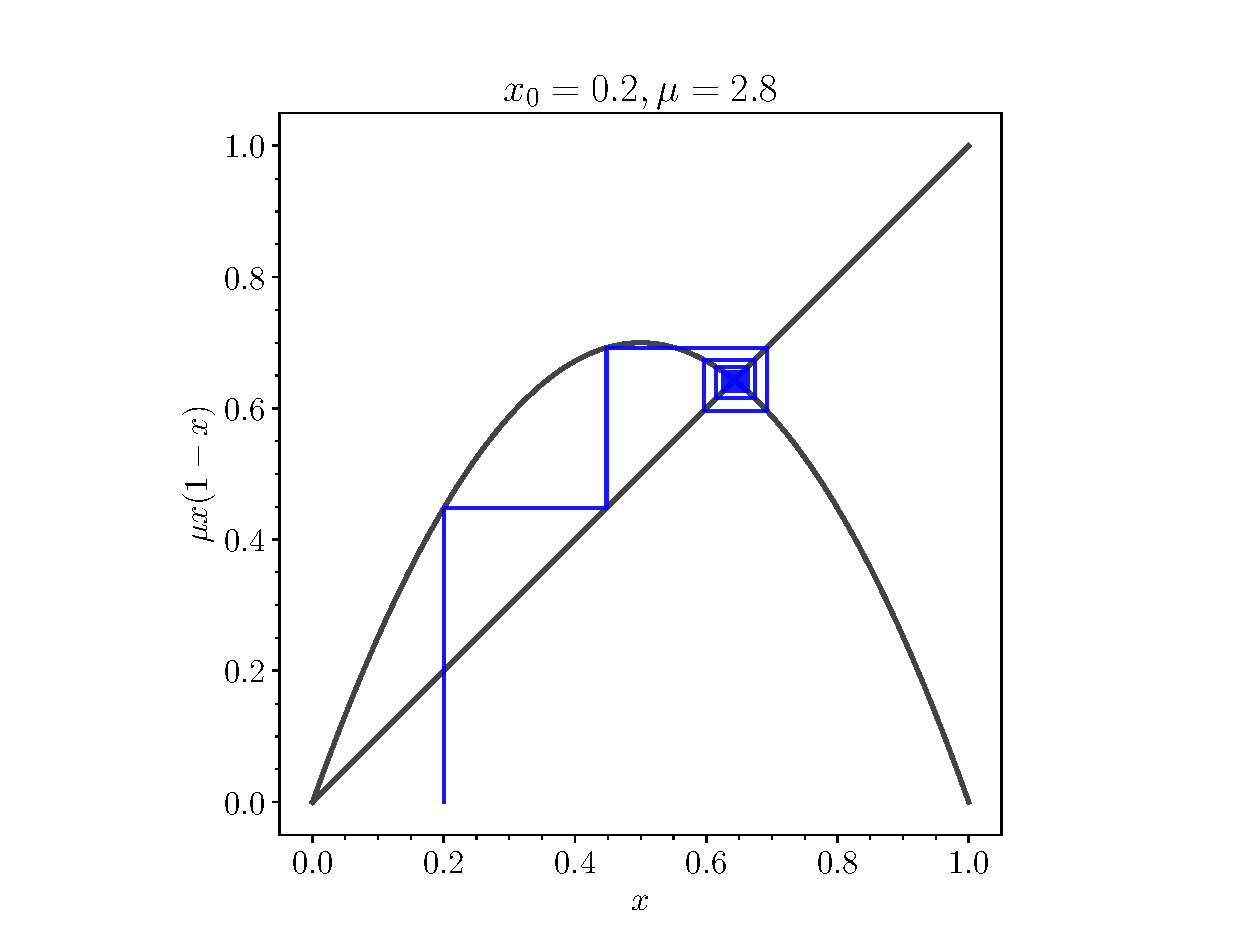
\includegraphics[scale=0.6]{cobweb_0.2_2.8}
\end{center}
\end{figure}

\begin{figure}
\begin{center}
\caption{Diagrama Cobweb de la ecuación logística, con $x_0=0.2$, $\mu=3.8$.}
\label{fig: cobweb_3.8}
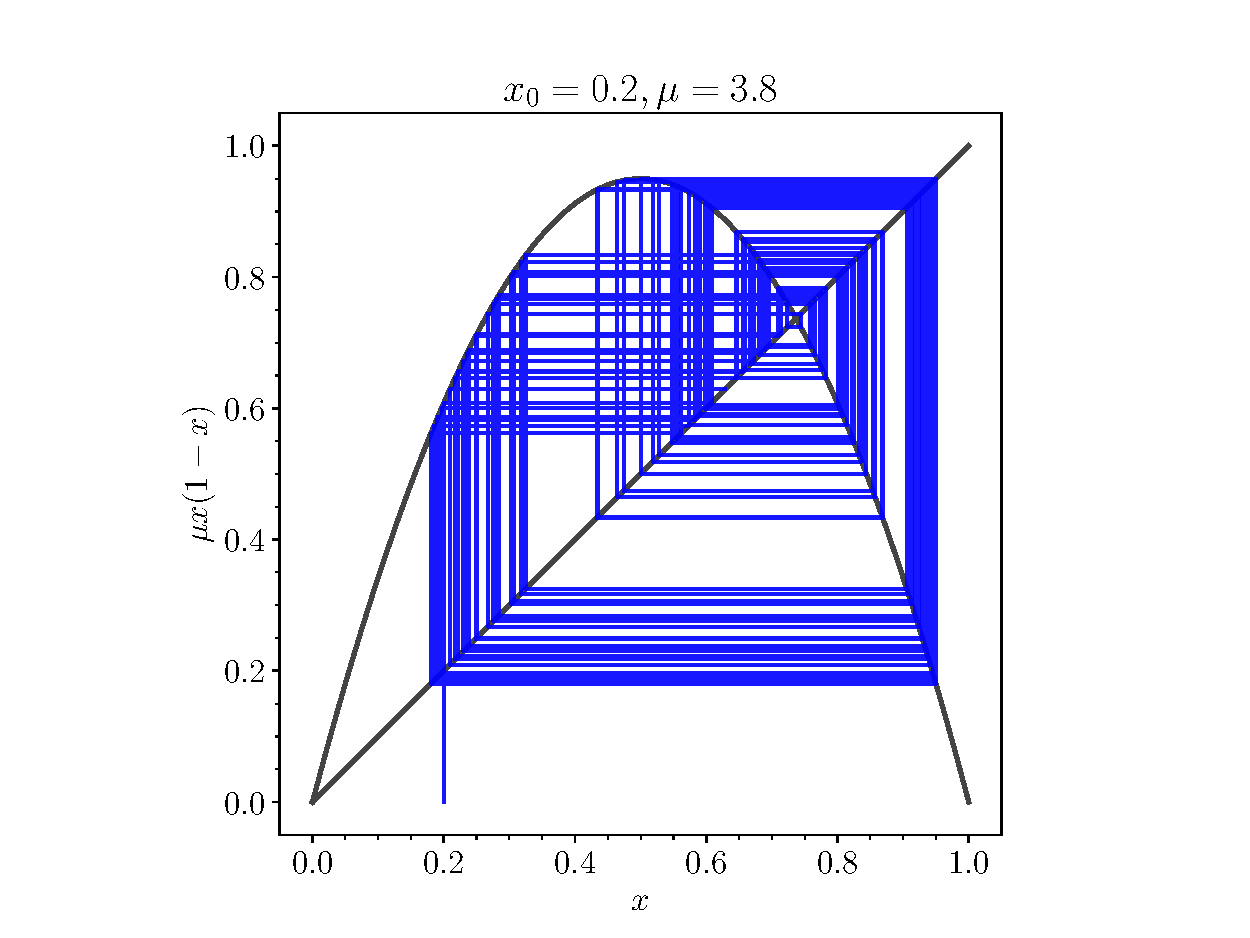
\includegraphics[scale=0.6]{cobweb_0.2_3.8}
\end{center}
\end{figure}

En \eqref{fig: cobweb_2.8} podemos ver como el punto de equilibrio $x^*=0$ es inestable y como el otro punto de equilibrio $x^*$ es localmente asintóticamente estable.

Asimismo, en \eqref{fig: cobweb_3.8} observamos como ambos puntos de equilibrio son inestables.

\end{proof}

\begin{proposition}
La ecuación logística tiene un 2-ciclo para todo $\mu > 3$, es decir, existen dos puntos $p$ y $q$ tal que $f(p)=q$ y $f(q)=p$.
\end{proposition}

\begin{proof}
Tenemos que $f(p)=q$ y $f(q)=p$ es equivalente a $f(f(p))=p$ y $f(f(q))=q$, es decir, $p$ es un punto fijo al iterar dos veces la función dada.

Como $f(x)$ es una función polinómica de segundo grado, entonces $f(f(x))$ será de cuarto grado, luego tendrá 4 raíces entre reales y complejas.

Por tanto necesitamos resolver la ecuación de cuarto grado $f(f(x))=x$. Sabemos que los puntos fijos de la ecuación logística cumplen $f(x^*)=x^*$, luego
$$f(f(x^*))=f(x^*)=x^*,$$
por lo que son solución de la ecuación. Y al factorizar conociendo estas soluciones el problema se reduce a resolver una ecuación cuadrática de la que obtenemos las siguientes raíces:
$$p,q=\frac{\mu+1\pm \sqrt{(\mu -3)(\mu +1)}}{2\mu}.$$

Estas soluciones son reales si $\mu > 3$ luego existe un 2-ciclo.

Si $\mu = 3$ estas raíces coinciden y valen $p=q=\frac{2}{3}=1-\frac{1}{3}=1-\frac{1}{\mu }$, luego no existe un 2-ciclo, hemos obtenido el mismo punto fijo.

Por último, si $\mu < 3$ las raíces no son reales y por tanto no existe un 2-ciclo.
\end{proof}

Si $\mu = 3.3$ tenemos  que la solución de la ecuación logística oscila repitiéndose cada dos iteraciones, es decir, sigue un 2-ciclo. Si $\mu = 3.5$ la solución se repite cada 4 iteraciones, luego sigue un 4-ciclo.
Se encuentran períodos más grandes (de 8, 16, 32...) a medida que $\mu$ toma valores mayores.

Sea $\mu_n$ el valor de $\mu$ para el cual aparece un $2^n$-ciclo. Entonces experimentalmente se obtiene que $\mu_n$ converge a un valor $\mu_\infty=3.569946...$.


\begin{proposition}
En la ecuación logística, se tiene que su solución converge si $\mu < 3$, oscila si $3 < \mu \lesssim 3.57$ y se produce caos si $\mu \gtrsim 3.57$. 
\end{proposition}


\section{Epidemiología}

Las enfermedades infecciosas como la influenza (o gripe) o la tuberculosis pueden ser severas. La epidemia del SIDA, pandemias recurrentes de influenza, brotes de ébola y la pandemia del Covid-19 son acontecimientos que preocupan e interesan a muchas personas. La prevalencia y los efectos de estas enfermedades sobre todo en países menos desarrollados son menos estudiadas, pero de mayor interés, pues la mortalidad de estas y otras enfermedades en estas zonas es mucho mayor que en países desarrollados. Muchas enfermedades como la malaria o el cólera son endémicas en muchas partes del mundo. Los efectos de enfermedades con alta mortalidad en la esperanza de vida y en la economía de los países afectados es considerable. Por ello, el estudio y modelado de epidemias es muy relevante.

A continuación se explican algunos conceptos básicos de epidemiología. Para esta sección se ha usado principalmente \cite{brauerMathematicalModelsPopulation2012}.

\begin{definition}
Las epidemias son brotes espontáneos de una enfermedad o situaciones endémicas, en las que la enfermedad está siempre presente.
\end{definition}

Los individuos de una población se pueden dividir en tres grupos, haciendo referencia a su situación con respecto a la enfermedad.

\begin{definition}
Los individuos \textbf{susceptibles}, que denotamos $S_n$, son aquellos que pueden infectarse con la enfermedad pero aún no lo han hecho en el momento $n$.
\end{definition}

\begin{definition}
Los individuos \textbf{infectados}, a los que denotamos $I_n$, son las personas infectadas en el instante $n$ por la enfermedad y pueden contagiar la enfermedad a los individuos susceptibles.
\end{definition}

\begin{definition}
Los individuos \textbf{recuperados}, que denotamos $R_n$, son los individuos que han estado infectados y ya no contagian la enfermedad ni pueden volver a infectarse.
Los individuos recuperados hacen referencia a los individuos inmunizados, aislados, recuperados o fallecidos.
\end{definition}

\section{Tipos de modelos epidemiológicos}

Los modelos epidemiológicos (principalmente SI, SIR y SIS) usan los estados Susceptible, Infectado y Recuperado. Los nombres suelen hacer referencia al flujo que se sigue para pasar entre los estados. Así, por ejemplo un modelo SI pasa de susceptible a infectado, uno SIR de susceptible a infectado y recuperado y SIS alterna entre susceptible e infectado.

En estos modelos se hacen dos suposiciones:
\begin{enumerate}
\item La población se mezcla de manera homogénea, es decir, todos los individuos tienen la misma probabilidad de contraer la enfermedad.
\item El total de la población es constante y lo denotaremos por $N$.
\end{enumerate}

\textcolor{red}{Añadir capitulo sobre los metodos de optimizacion}


\chapter{Modelos básicos en epidemiología}

\section{Tipos de modelos}

Los modelos discretos (principalmente SI, SIR y SIS) usan los estados Susceptible, Infectado y Recuperado. Los nombres suelen hacer referencia al flujo que se sigue para pasar entre los estados. Así, por ejemplo un modelo SI pasa de susceptible a infectado, uno SIR de susceptible a infectado y recuperado y SIS alterna entre susceptible e infectado.

En estos modelos se hacen dos suposiciones:
\begin{enumerate}
\item La población se mezcla de manera homogénea, es decir, todos los individuos tienen la misma probabilidad de contraer la enfermedad.
\item El total de la población es constante y lo denotaremos por $N$.
\end{enumerate}

En este capítulo estudiaremos los principales modelos epidemiológicos discretos y sus equivalentes continuos.

\section{Modelo SI}
El modelo SI es el modelo más simple de todos. Los individuos nacen siendo susceptibles a una enfermedad, una vez infectados no hay tratamiento y permanecen infectados el resto de su vida.
Un ejemplo de una enfermedad que pueda modelarse usando SI es el herpes.

Las siguientes ecuaciones describen el modelo SI discreto:

\begin{equation}
\label{eqn: SI}
\begin{aligned}
S_{n+1}=S_n\left( 1-\frac{\alpha\Delta t}{N}I_n\right) \\
I_{n+1}=I_n\left( 1+\frac{\alpha\Delta t}{N}S_n\right)
\end{aligned}
\end{equation}

donde $S_n$ indica el número de individuos susceptibles en el instante $t_n$, así como $I_n$ hace referencia al número de individuos infectados en ese instante. $\Delta t$ es el tiempo transcurrido entre dos instantes $t_{n+1}-t_n$ y N es el tamaño total de la población, con condiciones iniciales $S_0>0$, $I_0>0$ y $S_0+I_0=N$.

En estas ecuaciones $\alpha$ es la tasa de contacto, esto es, el número medio de individuos con los que un infectado tiene suficiente contacto para contagiarlo en un intervalo de tiempo. Por tanto, $S_n$ representa el número de individuos susceptibles en el tiempo $n\Delta t$.

Ahora, imponemos las suposiciones descritas anteriormente para estos modelos. En primer lugar, suponemos que la población se mezcla de manera homogénea de ahora en adelante, y para la segunda, la población total se mantiene constante,  es trivial que se cumpla siempre, ya que sumando el sistema de ecuaciones el resultado es $N$ y asumimos que las soluciones son siempre positivas pues las soluciones negativas no tienen sentido.
Además, no tiene sentido hablar de un número negativo de individuos, ya sean infectados, recuperados o susceptibles de contraer la enfermedad.

\begin{proposition}
Las soluciones de las ecuaciones \eqref{eqn: SI} son positivas si y solo si $\alpha\Delta t \leq 1$.
\end{proposition}

\begin{proof}
Supongamos que $I_n, S_n > 0$. Por la segunda ecuación del modelo \eqref{eqn: SI} es claro que $I_{n+1}>0$, pues $S_n>0$ y $1+\frac{\alpha\Delta t}{N}>0$.

Para la primera ecuación tenemos que 
$$S_{n+1}>0 \Leftrightarrow 1-\frac{\alpha\Delta t}{N}I_n >0,$$

ya que $I_n$ es positivo por hipótesis. Esto equivale a:
$$N>\alpha\Delta t(N-S_n) \Leftrightarrow \alpha\Delta t S_n > (\alpha\Delta t -1) N.$$

Como $\alpha\Delta t S_n > 0$, tenemos entonces que la desigualdad se da si y solo si:
$$\alpha\Delta t -1 \leq 0 \Leftrightarrow \alpha\Delta t \leq 1.$$
\end{proof}


Buscamos ahora ver cual es el comportamiento del sistema, calculando los puntos de equilibrio, esto es, las soluciones constantes en el tiempo, para lo que resolvemos:

$$
\begin{cases}
S^*=S^*\left( 1-\frac{\alpha\Delta t}{N}I^*\right) \\
I^*=I^*\left( 1+\frac{\alpha\Delta t}{N}S^*\right) \\
S^*+I^*=N
\end{cases}
$$

Los únicos puntos de equilibrio posibles son: $S^*=0, I^*=N$ y $S^*=N, I^*=0$, y como sabemos que tenemos condiciones iniciales positivas y es claro que $S_n$ es monótonamente decreciente e $I_n$ es monótonamente creciente, ya que $S_{n+1}$ es $S_n$ multiplicado por un valor menor que $1$, mientras que $I_{n+1}$ corresponde a $I_n$ multiplicado por un valor mayor que $1$, así $S_{n+1}<S_n$ y $I_{n+1}>I_n$ para cualquier $n\in\mathbb{N}$, entonces debe converger a $S^*=0, I^*=N$, pues son sucesiones monótonas acotadas.

Expresando $\alpha$ como una tasa podemos obtener las ecuaciones diferenciales análogas de la siguiente manera. Considerando

$$\frac{S_{n+1} - S_n}{\Delta t} \approx S'(t),$$

El análogo continuo al sistema \eqref{eqn: SI} viene dado por:

\begin{equation}
\begin{aligned}
S'(t) = -\frac{\alpha}{N}SI \\
I'(t) = \frac{\alpha}{N}SI
\end{aligned}
\end{equation}

con condiciones iniciales $S(0)+I(0)=N$.

De manera análoga al caso discreto calculamos los puntos de equilibrio, es decir, suponemos que las funciones son constantes y resolviendo el sistema de ecuaciones, podemos comprobar que las soluciones convergen a $S^*=0, I^*=N$ y, por tanto, tienen el mismo comportamiento que el caso discreto.

Sustituyendo en el modelo $S=N-I$ obtenemos la ecuación diferencial logística

$$I'(t) = I\frac{\alpha}{N}(N-I).$$

Esta ecuación diferencial se puede resolver por separación de variables como sigue:

\begin{equation}
\begin{aligned}
I'(t)=I\frac{\alpha}{N}(N-I(t)) & \Leftrightarrow \int \frac{dI}{I(N-I)} = \int \frac{\alpha}{N} dt \\
& \Leftrightarrow \frac{1}{N}\int (\frac{1}{I}+\frac{1}{N-I}dI = \frac{\alpha}{N}t+c \\
& \Leftrightarrow  \frac{1}{N}\log{\frac{I}{N-I}} = e^{\frac{\alpha}{N}t+c} \\
& \Leftrightarrow  \frac{I}{N-I} = e^ce^{\alpha t} \\
& \Leftrightarrow  I = e^ce^{\alpha t}(N-I) \\
& \Leftrightarrow  I(1+e^ce^{\alpha t} = e^ce^{\alpha t}N \\
& \Leftrightarrow  I(t) = \frac{e^ce^{\alpha t}N}{1+e^ce^{\alpha t} }
\end{aligned}
\end{equation}

Ahora usando el valor inicial $I(0)$ tenemos:

\begin{equation}
\begin{aligned}
I(0) = \frac{e^cN}{1+e^c} & \Leftrightarrow (1+e^c)I(0) = e^cN \\
& \Leftrightarrow e^c(N-I(0)) = I(0) \\
& \Leftrightarrow e^c = \frac{I(0)}{N-I(0)}
\end {aligned}
\end{equation}

luego la solución general es:

$$I(t) = \frac{I(0)e^{\alpha t}N}{(N-I(0))+I(0)e^{\alpha t}} = \frac{I(0)N}{(N-I(0))e^{-\alpha t}+I(0)}$$

Es claro que $I$ se tiende monótonamente a $N$, luego tiene el mismo comportamiento que el modelo discreto.


\begin{figure}
\begin{center}
\caption{Gráfica del modelo SI, en una población total de $100$ individuos, con valores iniciales $S_0=99, I_0 = 1, \alpha = 0.1, T_0 = 0, T = 100$.}
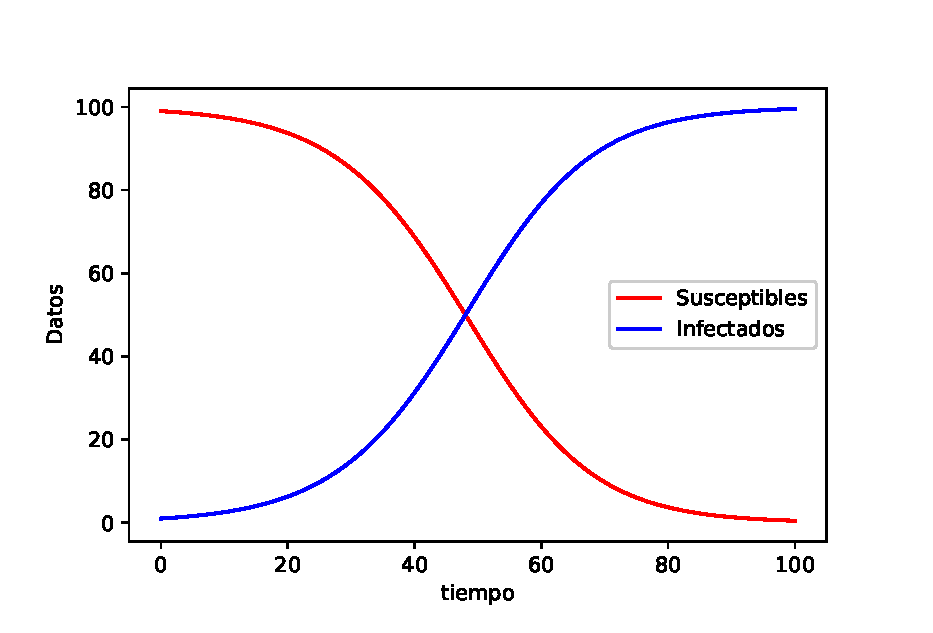
\includegraphics[scale=1]{graficaSI}
\end{center}
\end{figure}

\begin{figure}
\begin{center}
\caption{Gráfica del modelo SI, representando el número de infectados según el número de individuos susceptibles, en una población total de $100$ individuos, con valores iniciales $S_0=99, I_0 = 1, \alpha = 0.1, T_0 = 0, T = 100$.}
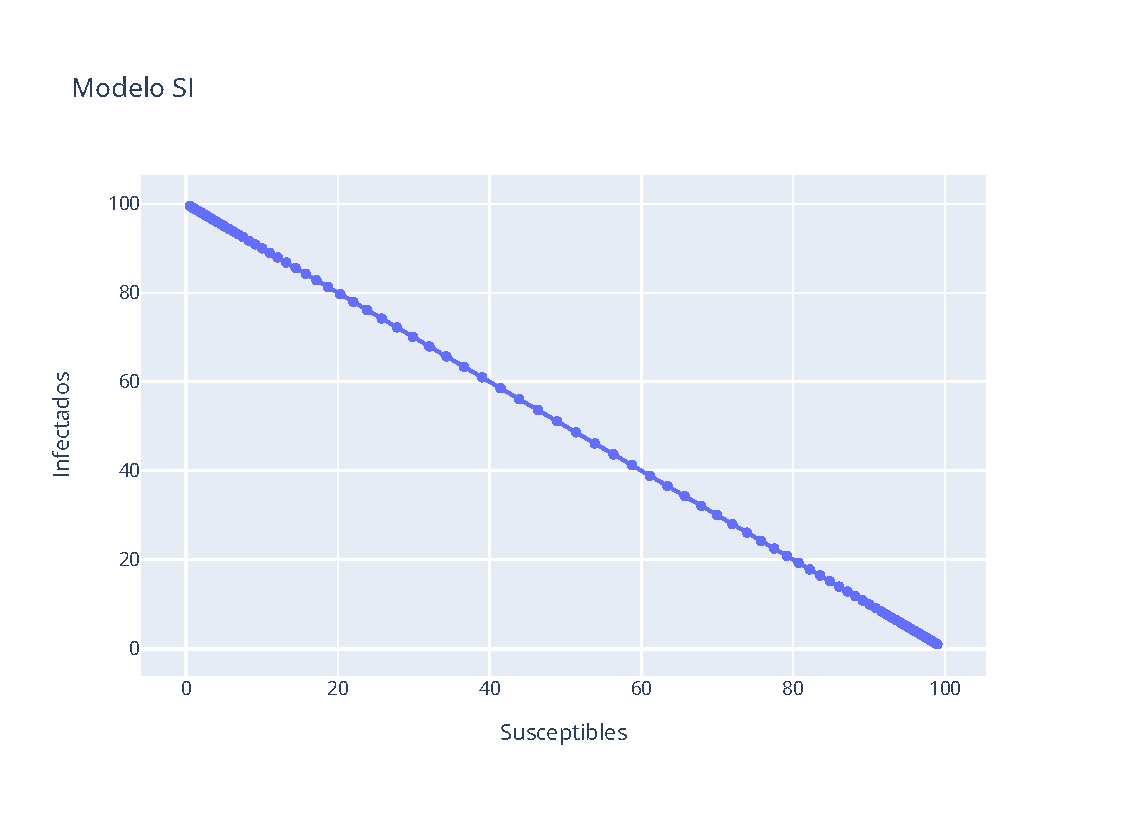
\includegraphics[scale=0.8]{SI_IsobreS}
\end{center}
\end{figure}

\section{Modelo SIR}
El modelo SIR comienza como el SI, pero tras infectarse los individuos pasan a un estado Recuperado, en el cual no pueden infectarse ni infectar a otros.
Un ejemplo de este tipo de enfermedad es la varicela. 

El modelo es el siguiente:

\begin{equation}
\label{eqn: SIR_modelo}
\begin{aligned}
S_{n+1} = & S_n \left(1-\frac{\alpha\Delta t}{N} I_n \right) \\
I_{n+1} = & I_n \left( 1-\gamma \Delta t + \frac{\alpha\Delta t}{N} S_n \right) \\
R_{n+1} = & R_n + \gamma \Delta t I_n
\end{aligned}
\end{equation}

con condiciones iniciales $S_0>0$, $I_0>0$, $R_0\geq 0$, satisfaciendo $S_0+I_0+R_0=N$.

En estas ecuaciones, de nuevo tenemos que $\alpha$ es la tasa de contacto, esto es, el número medio de individuos con los que un infectado tiene suficiente contacto para contagiarlo en un intervalo de tiempo y $\gamma$ es la probabilidad de que un infectado pase a recuperado/retirado/aislado/fallecido en un intervalo de tiempo, con $\alpha >0$ y $\gamma >0$.

Se supone que la población permanece constante, $S_n+I_n+R_n=N$.

\begin{proposition}
Las soluciones a este sistema discreto son positivas para cualquier valor de las condiciones iniciales si, y solo si:
$$\max{\big\{\gamma\Delta t, \alpha\Delta t\big\} } \leq 1$$

o equivalentemente:

$$\min{\bigg\{ \frac{1}{\gamma}, \frac{1}{\alpha} \bigg\} } \geq \Delta t$$

\end{proposition}

\begin{proof}
Comenzamos probando una de las implicaciones, supongamos que $\max{\big\{\gamma\Delta t, \alpha\Delta t\big\} } \leq 1$.

Por hipótesis inicial, tenemos que $S_0, I_0, R_0>0$ y $S_0+I_0+R_0=N$, luego basta ver que:
$$(1-\frac{\alpha \Delta t}{N}I_0)>0.$$
Lo cual es evidente, pues $\frac{I_n}{N}<1$ por hipótesis del modelo y $\alpha \Delta t<1$.

Por un razonamiento análogo, tenemos que $$1-\gamma \Delta t+\frac{\alpha\Delta t}{N}S_0 > 0.$$
Y finalmente $$R_0+\gamma\Delta t I_0>0$$ pues $\gamma>0$ y $\Delta t <0$.

Ahora, por inducción, suponiéndolo para $n$ se puede demostrar que $S_{n+1}, I_{n+1}, R_{n+1}$ son siempre positivas por razonamiento análogo.

Para probar el recíproco basta probar que ambas cantidades son menores o iguales a $1$, comenzamos trabajando en la primera ecuación, suponemos la positividad para $n$ y queremos probarla para $n+1$:
$$S_{n+1}=S_n\left(1-\frac{\alpha\Delta t}{N}I_n\right)$$
como $S_n>0$ basta ver que $1-\frac{\alpha\Delta t}{N}I_n>0$. Usamos de nuevo que $I_n \leq N$ y entonces tenemos:
$$1-\frac{\alpha\Delta t}{N}I_n \leq 1-\alpha\Delta t,$$
por tanto:
$$1-\alpha\Delta t > 0 \Leftrightarrow \alpha\Delta t  \leq 1.$$

En la segunda ecuación, como sabemos que $S_n$ es estrictamente decreciente, pues es una sucesión de la forma $X_{n+1}=\beta X_n$ con $\beta < 1$, entonces es cada vez más pequeño y el factor
$\frac{\alpha \Delta t}{N}S_n$ tiende a cero. \textcolor{red}{No estoy muy segura de este paso, pero si lo hago despejando me sale que debe ser menor que 2 y no que 1 :(}
Luego despejando como antes tenemos $\gamma\Delta t \leq 1$.

De la última ecuación no sacamos ninguna condición más, pues su solución es siempre positiva por definición de $\gamma$ y $\Delta t$.

\end{proof}

Por tanto, el intervalo de tiempo debe ser menor que el tiempo medio requerido para un contacto exitoso y menor que el período medio infeccioso.
% Con contacto exitoso asumo que se refiere al tiempo necesario para infectar a un individuo. Sí es esto confirmado por la profe

El comportamiento global del sistema es fácil de ver. Definimos la tasa reproductiva como la constante 
$$\mathcal{R}_{SIR}=\frac{S_0 \alpha}{N\gamma }.$$

El valor de $\mathcal{R}_{SIR}$ determina el comportamiento global del modelo.

En otros trabajos como \cite{demongeotSIEpidemicModel} esta tasa reproductiva se llama tasa de transmisión media.

Notemos que $S_n$ es estrictamente decreciente y $R_n$ es estrictamente creciente. Estudiémoslas:

Sea $S_\infty=\lim_{n\rightarrow\infty} S_n\geq 0$, cuyo límite existe pues es una sucesión estrictamente decreciente y acotada inferiormente por $0$. Estudiamos las condiciones iniciales. Si $S_0\leq \frac{\gamma N}{\alpha}$, o, equivalentemente, $\mathcal{R}_{SIR}˘\leq 1$ entonces $I_1\leq I_0$ y, como $S_n$ es estrictamente decreciente, tenemos que $I_{n+1}\leq I_n$, es decir, no hay epidemia. En otro caso, tenemos $S_0> \frac{\gamma N}{\alpha}$, entonces $I_1>I_0$. Debe ocurrir que $S_\infty <\frac{N\gamma}{\alpha}$, pues si no fuera así, tendríamos que $I_n$ crece hacia un equilibrio, $I_\infty$, lo que implica que $R_n$ se aproxima a infinito cuando $n\rightarrow\infty$, lo cual no es posible. Así, el número de infectados finalmente comienza a decrecer y se aproxima a $0$. Además, sabemos por el Lema 1 de \cite{allenDiscretetimeSISIR1994} que $S_\infty>0$.

El modelo continuo correspondiente al modelo SIR se comporta de la misma forma que el modelo discreto, este sería:

\begin{equation}
\label{eqn: modelo_SIR_continuo}
\begin{cases}
S'(t) = -\dfrac{\alpha}{N}SI \\
I'(t) = I\left(\dfrac{\alpha}{N}S-\gamma \right) \\
R'(t) = R+\gamma I
\end{cases}
\end{equation}

donde $S(0)+I(0)+R(0)=N$. La tasa reproductiva en este caso se define como
$$\mathcal{R}_{SIR}=\frac{S(0)\alpha }{N\gamma },$$
y si como hemos visto $\mathcal{R}_{SIR}\leq 1$  no hay epidemia, pero en cambio, si es mayor, hay epidemia.

\begin{figure}
\begin{center}
\caption{Gráfica del modelo SIR, en una población total de $100$ individuos, con valores iniciales $S_0=99, I_0 = 1, R_0 = 0, \alpha = 0.1, \gamma = 0.01 T_0 = 0, T = 300$.}
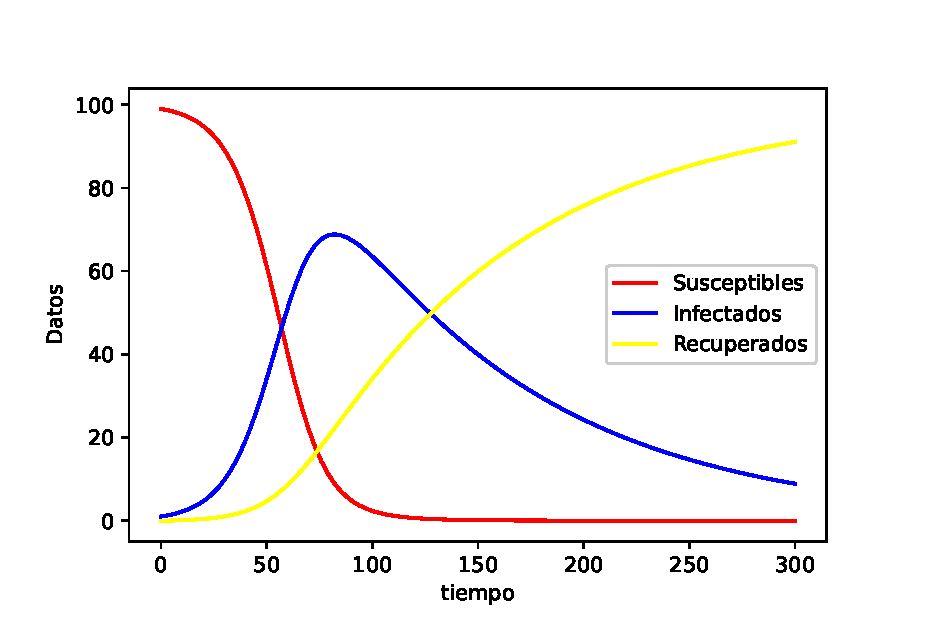
\includegraphics[scale=1]{graficaSIR}
\end{center}
\end{figure}

\begin{figure}
\begin{center}
\caption{Gráfica del modelo SI, representando el número de infectados según el número de individuos susceptibles, en una población total de $100$ individuos, con valores iniciales $S_0=99, I_0 = 1, \alpha = 0.1, \gamma=0.01, T_0 = 0, T = 300$.}
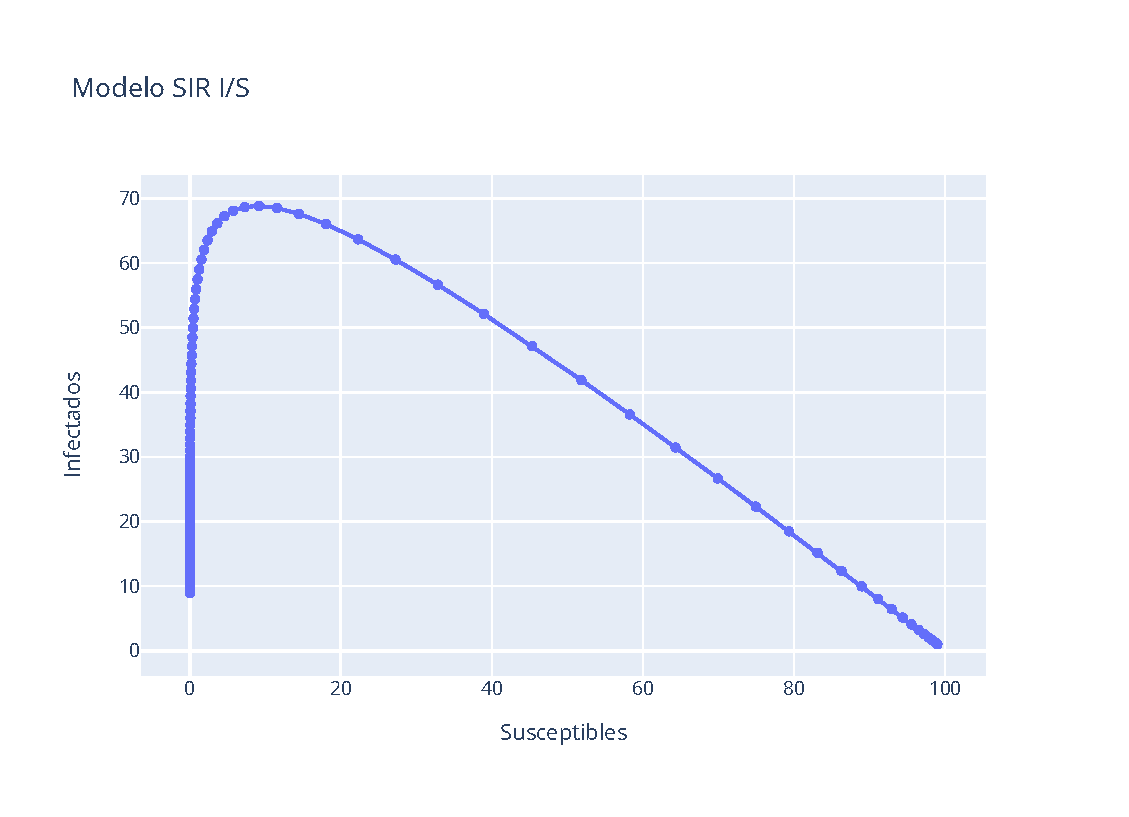
\includegraphics[scale=0.8]{SIR_IsobreS}
\end{center}
\end{figure}

\begin{figure}
\begin{center}
\caption{Gráfica del modelo SIR, representando el número de recuperados según el número de individuos susceptibles, en una población total de $100$ individuos, con valores iniciales $S_0=99, I_0 = 1, \alpha = 0.1, \gamma=0.01, T_0 = 0, T = 300$.}
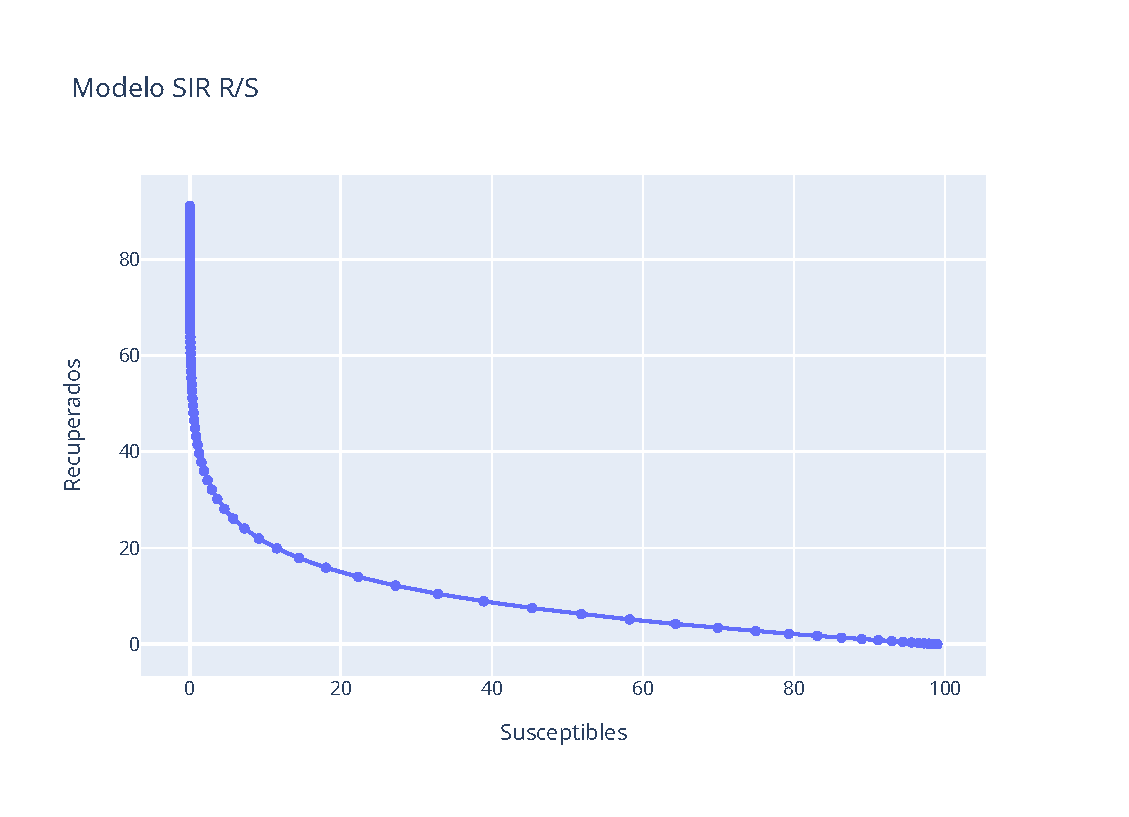
\includegraphics[scale=0.8]{SIR_RsobreS}
\end{center}
\end{figure}

\begin{figure}
\begin{center}
\caption{Gráfica del modelo SI, representando el número de recuperados según el número de individuos infectados, en una población total de $100$ individuos, con valores iniciales $S_0=99, I_0 = 1, \alpha = 0.1, \gamma=0.01, T_0 = 0, T = 300$.}
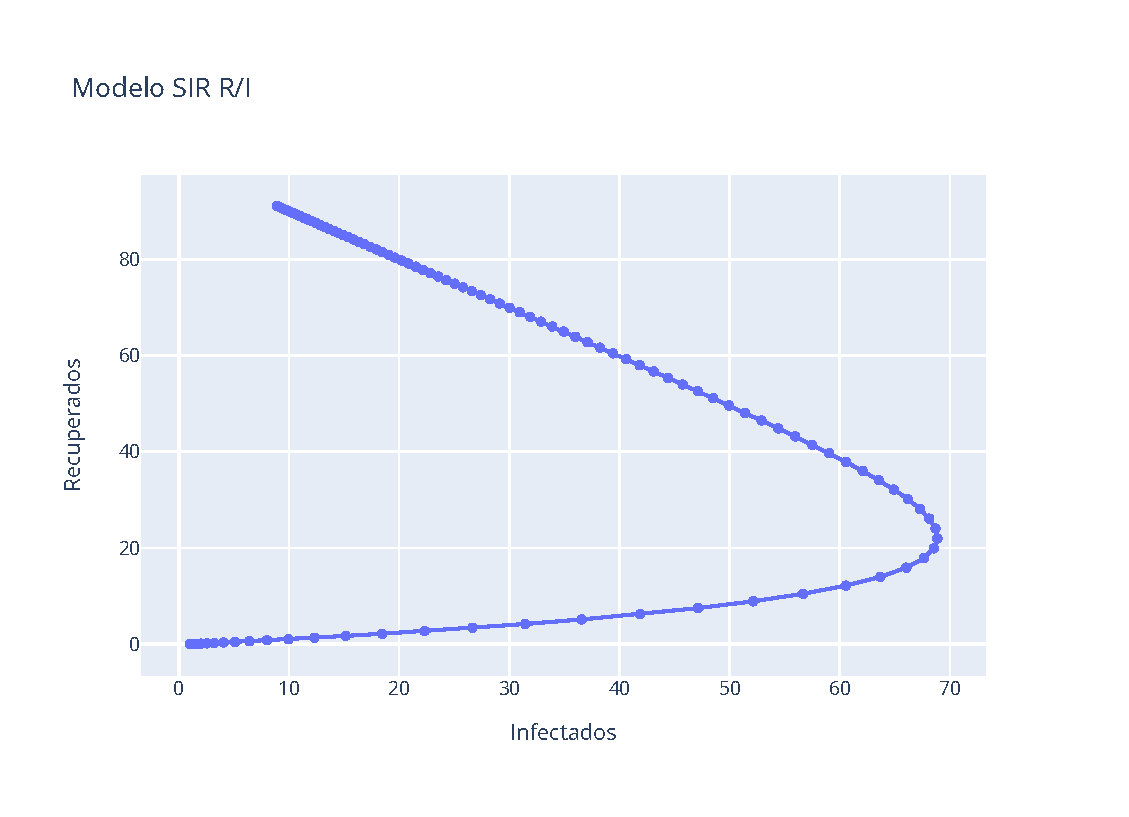
\includegraphics[scale=0.8]{SIR_RsobreI}
\end{center}
\end{figure}


\section{Modelo SIS}
El modelo SIS es similar al SI, con la salvedad de que los individuos son susceptibles de múltiples infecciones.
Por ejemplo, los resfriados pueden modelarse usando SIS.

El modelo es una perturbación del modelo SI visto antes, se define de la siguiente forma:

\begin{equation}
\label{eqn: modelo_SIS}
\begin{aligned}
S_{n+1} = S_n \left(1-\frac{\alpha\Delta t}{N} I_n \right) + \gamma \Delta t I_n \\
I_{n+1} = I_n \left( 1-\gamma \Delta t + \frac{\alpha\Delta t}{N} S_n \right)
\end{aligned}
\end{equation}

con condiciones iniciales positivas $S_0>0$, $I_0>0$ cumpliendo $S_0+I_0=N$. Por lo tanto, el tamaño de la población es constante.

En estas ecuaciones, $\alpha$ de nuevo representa la tasa de contacto, esto es, el número medio de individuos con los que un infectado tiene suficiente contacto para contagiarlo en un intervalo de tiempo y $\gamma$ es la probabilidad de que un infectado pase a recuperado/retirado/aislado/fallecido en un intervalo de tiempo, donde se cumple $\alpha >0$ y $\gamma >0$.

\begin{proposition}
Las soluciones de \eqref{eqn: modelo_SIS} siempre son positivas si, y solo si:

$$\gamma \Delta t \leq 1 $$ y $$\alpha\Delta t< \left( 1+\sqrt{\gamma \Delta t} \right)^2$$

\end{proposition}
\begin{proof}
Sea $I_0=\epsilon$ y $S_0=N-\epsilon$, entonces por la definición del modelo tenemos:
\begin{equation}
\begin{aligned}
I_1 & =\epsilon\left(1-\gamma\Delta t+\alpha\Delta t\frac{N-\epsilon}{N}\right) \\
& = -\frac{\alpha\Delta t \epsilon^2}{N} + \epsilon(1-\gamma\Delta t+\alpha\Delta t ) \\
& = p(\epsilon) \\
\end{aligned}
\end{equation}

Luego tenemos que ver cuando la parábola satisface $0<p(\epsilon)<N$ para $0<\epsilon<N$.

Notemos que $p(0)=0$ y $p(N)=N(1-\gamma\Delta t$.

Sea $(\epsilon^*, p^*)$ el vértice de la parábola, entonces 
$$(\epsilon^*, p^*) = \left(\frac{N(1-\gamma\Delta t+\alpha\Delta t)}{2\alpha\Delta t}, \frac{N(1-\gamma\Delta t+\alpha\Delta t)^2}{4\alpha\Delta t}\right)$$

Por tanto, $0<p(\epsilon )<N$ para $0<\epsilon <N$ si y solo si:

$$\gamma\Delta t \leq 1,$$

y por tanto, o bien $\epsilon^* \geq N$, que es equivalente a $\alpha\Delta t \leq 1-\gamma\Delta t$.

O bien $\epsilon^*<N \text{  y  } p^*<N$, lo que requiere que $\alpha\Delta t > 1-\gamma\Delta t$ y $(1-\gamma\Delta t+\alpha\Delta t)^2<4\alpha\Delta t$. Estas desigualdades se dan si y solo si:

$$1-\gamma\Delta t < \alpha \Delta t < \left( 1+\sqrt{\gamma \Delta t} \right)^2$$

\end{proof}

En el modelo SIS, la tasa reproductiva se define como 
$$\mathcal{R}_{SIS}=\frac{\alpha}{\gamma}.$$

Si $\mathcal{R}_{SIS}\leq 1$ entonces se tiene que $I_{n+1} < I_n$, ya que $0<S_n<N$ y las soluciones son positivas. En este caso es fácil ver que el límite, al ser una sucesión monótona decreciente y acotada inferiormente, es $(S^*,I^*)=(N,0)$. Supongamos que $S^*<N$, entonces existen $n_1, \epsilon$ tales que para todo $n \geq n_1$:
$$S_n<S^*+\epsilon < N$$
y usando las ecuaciones \eqref{eqn: modelo_SIS}
$$I_{n+1} \leq I_n \left( 1-\gamma \Delta t + \frac{\alpha\Delta t}{N} S_n \right) = \rho I_n$$

Como $\rho < 1$ tendríamos que $I^*=0$, lo que contradice que $S^*<N$.

Si $\mathcal{R}_{SIS}>1$ realizando la sustitución $S_n=N-I_n$ y el cambio

$$x_n=\frac{\alpha \Delta t I_n}{N(1+\alpha \Delta t - \gamma \Delta t)}$$

tenemos:

\begin{equation}
\begin{aligned}
\alpha\Delta t I_n = x_nN(1+\alpha\Delta t-\gamma\Delta t) \Leftrightarrow \\
I_n = x_n\frac{N(1+\alpha\Delta t - \gamma\Delta t}{\alpha\Delta t}
\end{aligned}
\end{equation}

entonces sustituyendo en la ecuación \eqref{eqn: modelo_SIS}:

\begin{equation}
\begin{aligned}
x_{n+1}\frac{N(1-\alpha\Delta t-\gamma\Delta t)}{\alpha \Delta t} = x_n\frac{N(1+\alpha\Delta t-\gamma \Delta t)}{\alpha\Delta t}\left( 1-\gamma\Delta t+\frac{\alpha\Delta t}{N}\left(N-x_n\frac{N(1+\alpha\Delta t-\gamma\Delta t)}{\alpha\Delta t}\right) \right)
\end{aligned}
\end{equation}

Despejando de esta expresión:

\begin{equation}
\begin{aligned}
x_{n+1} & = x_n\left( 1-\gamma\Delta t+\frac{\alpha\Delta t}{N}N-\frac{\alpha\Delta t}{N}x_n\frac{N(1+\alpha\Delta t -\gamma \Delta t)}{\alpha\Delta t} \right) \\
& = x_n(1-\gamma\Delta t + \alpha\Delta t -x_n(1+\alpha\Delta t -\gamma\Delta t)) \\
& = x_n((1-\gamma\Delta t+\alpha\Delta t)(1-x_n))
\end{aligned}
\end{equation}

luego obtenemos la ecuación logística

$$x_{n+1} = (1+\alpha \Delta t - \gamma \Delta t)x_n(1-x_n)$$

De este la restricción necesaria para garantizar soluciones positivas no es suficiente para asegurar la convergencia, en este caso a dicha restricción hay que añadir la condición $\alpha \Delta t \leq 2+\gamma \Delta t$.


\begin{figure}
\begin{center}
\caption{Gráfica del modelo SIS, en una población total de $100$ individuos, con valores iniciales $S_0=95, I_0 = 5, \alpha = 0.1, \gamma=0.01, T_0 = 0, T = 150$.}
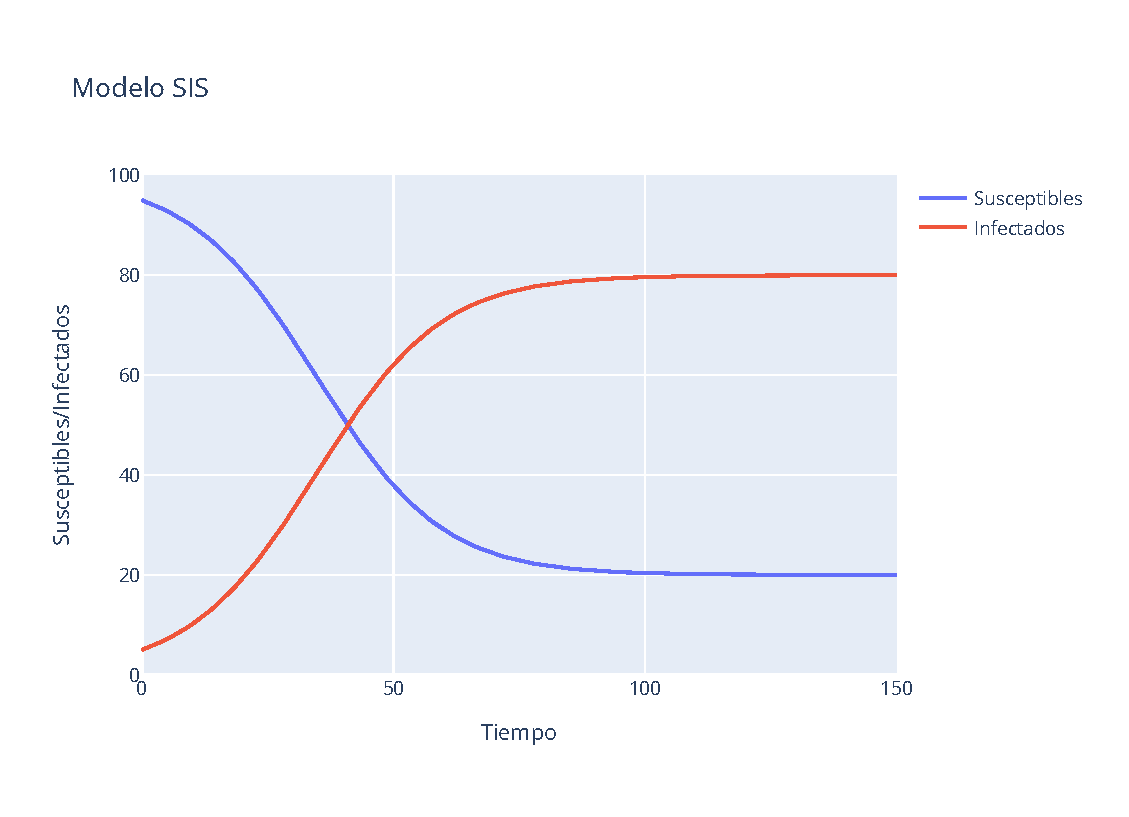
\includegraphics[scale=0.8]{SIS_modelo}
\end{center}
\end{figure}

\begin{figure}
\begin{center}
\caption{Gráfica del modelo SIS, representando el número de infectados según el número de individuos susceptibles, en una población total de $100$ individuos, con valores iniciales $S_0=95, I_0 = 5, \alpha = 0.1, \gamma=0.01, T_0 = 0, T = 200$.}
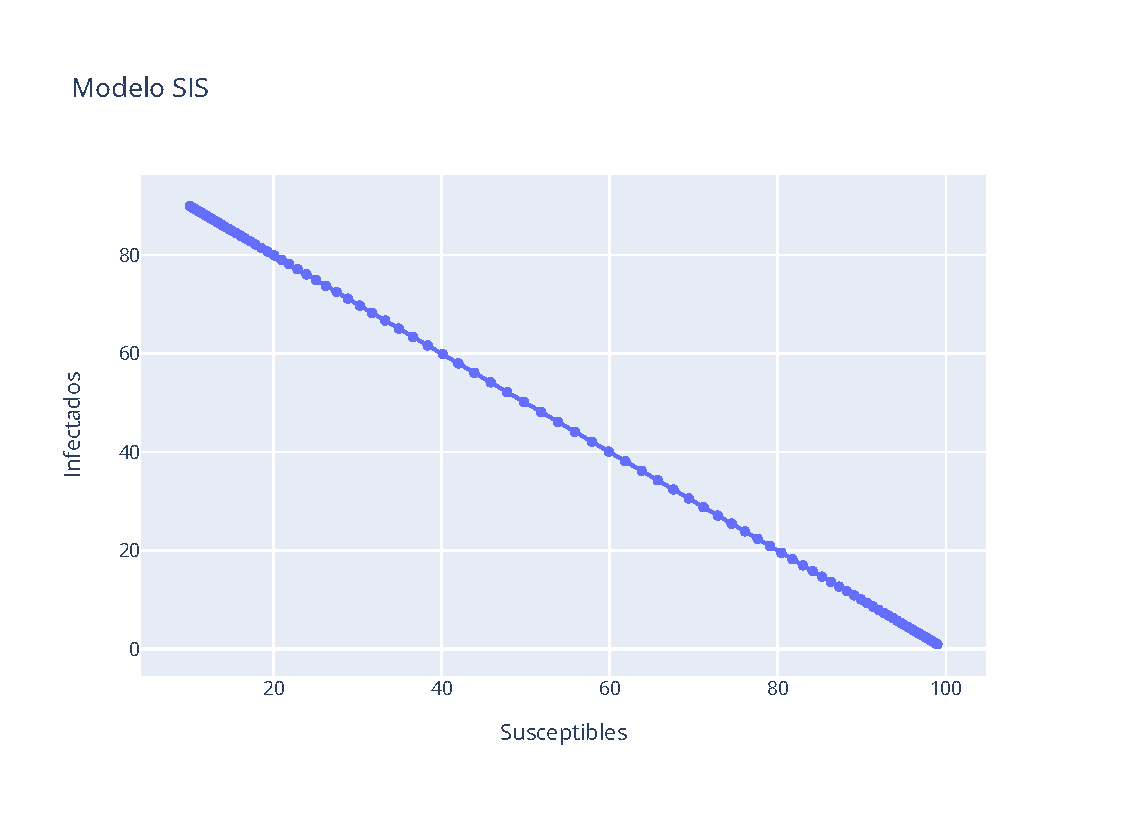
\includegraphics[scale=0.8]{SIS_IsobreS}
\end{center}
\end{figure}







\section{Análisis de los parámetros de los modelos}

\subsection{Introducción}

Estimar la tasa de transmisión media es uno de los aspectos más cruciales en epidemiología. Esta tasa condiciona la fase de la epidemia e incluso si va a extinguirse. Es combinación de tres factores:

\begin{enumerate}
\item Coeficiente de virulencia: Relacionado con el agente infeccioso.
\item Coeficiente de susceptibilidad: Relacionado con el anfitrión.
\item Número de contactos por unidad de tiempo entre individuos.
\end{enumerate}

Los dos primeros factores se tienen en cuenta a la vez en la probabilidad de transmisión.

Todos los factores pueden cambiar con el tiempo, el primero debido a mutaciones del virus y los dos últimos por medidas de contención. Por tanto, observar el decrecimiento de la transmisión media en una enfermedad es una buena forma de comprobar la efectividad de las medidas de contención.

En el artículo \cite{demongeotSIEpidemicModel} se presenta un modelo SI modificado con el objetivo de compararlo con los datos obtenidos en la pandemia de la COVID-19 hasta el momento y así tratar de predecir su comportamiento en el futuro.

El modelo SI continuo considerado es el siguiente:

\begin{equation}
\label{eqn: SI_cont}
\begin{aligned}
S'(t) = -\tau (t)S(t)I(t) \\
I'(t) = \tau (t)S(t)I(t) -vI(t)
\end{aligned}
\end{equation}

donde $S(t)$ es el número de individuos susceptibles , $I(t)$ el número de individuos infectados en el tiempo $t$ y $\tau (t)$ la tasa de transmisión, que combina el número de contactos por unidad de tiempo y la probabilidad de transmisión. Observemos que $\tau (t)$ se considera variable respecto al tiempo, al contrario que en el caso SI clásico estudiado antes. Además, notemos que $v$ es una constante, donde $1/v$ es la duración media del período de infección, y $vI(t)$ el flujo de individuos recuperados o fallecidos. %vI(t) es el flujo de recuperados o muertos porque ha mezclado el modelo SI y SIR; vI(t) serian los recuperados, pero se ahorra la ecuacion de la R

Se consideran las condiciones iniciales

$$S(t_0)=S_0>0, \: I(t_0)=I_0>0$$

Ahora, consideramos que al final del período infeccioso nos han informado de una fracción del total de casos, en este caso la fracción la denotamos por $f\in (0,1]$. Sea $C_R(t)$ el número total acumulado de casos reportados. Entonces:

\begin{equation}
\label{eqn: acumulada}
C_R(t) = {C_R}_0 + vfC_I(t) \; \forall t \geq t_0
\end{equation}

donde $C_{R0}$ representa el número de casos reportados al inicio del estudio y 

\textcolor{red}{¿Por qué $vfC_I(t)$ va multiplicado por $v$?}

$$C_I(t) = \int_{t_0}^t I(w) dw $$

siendo $C_I$ el número total de infectados acumulado.

Asumimos conocidos $S_0 > 0$, $1/v>0$, $f\in (0,1]$. Por tanto, queremos averiguar el número inicial de infectados $I_0$ y la tasa de transmisión $\tau (t)$.

\subsection{Aproximando $I_0$ y $\tau (t_0)$}
Ahora, procedemos a intentar aproximar $I_0$ y $\tau (t_0)$:

Al comienzo de la pandemia podemos asumir que $S(t)$ y $\tau (t)$ son constantes e iguales a $S_0$ y $\tau_0 = \tau (t_0)$ respectivamente. Así, sustituyendo estos valores en la ecuación \eqref{eqn: SI_cont} obtenemos:

$$I'(t) = (\tau_0 S_0 -v) I(t).$$

Resolviendo la ecuación diferencial llegamos a:

$$I(t) = I_0\exp{((\tau_0 S_0-v)(t-t_0))}.$$

Sustituyendo en \eqref{eqn: acumulada}:

$$C_R(t) = {C_R}_0 + vfI_0\frac{\mathrm{e}^{(\tau_0 S_0 -v)(t-t_0)} -1}{\tau_0 S_0-v}$$

Así, hemos obtenido un primer modelo para los casos acumulados al principio de la pandemia.

Reescribimos la ecuación anterior como:

\begin{equation}
\label{eqn: acumulada_modelo}
C_R(t) = \chi_1 \mathrm{e}^{\chi_2 t} -\chi_3
\end{equation}

Estimamos $\chi_3$ usando los datos de la epidemia obtenidos, y el mejor ajuste para los datos es $\chi_3=0$.

Ahora, usando \eqref{eqn: acumulada} y \eqref{eqn: acumulada_modelo} tenemos:

\begin{equation}
I_0=\frac{\chi_1\chi_2\mathrm{e}^{\chi_2 t_0}}{vf}
\end{equation}

Y, como de reescribir sabemos que $\chi_2 = \tau_0 S_0-v$, entonces

\begin{equation}
\tau_0 = \frac{\chi_2+v}{S_0}
\end{equation}

Si suponemos que $\tau (t) = \tau_0$ constante, tenemos que el modelo queda:

\begin{equation}
\begin{aligned}
S'(t) = -\tau_0S(t)I(t) \\
I'(t) = \tau_0S(t)I(t) -vI(t)
\end{aligned}
\end{equation}

Usando la ecuación de $S(t)$ y resolviéndola obtenemos:

$$S(t) = S_0\exp{\left( -\tau_0 \int_{t_0}^t I(w) dw \right)} = S_0\exp{(-\tau_0 C_I(t))}$$

Ahora, sustituyendo esta expresión en la ecuación de $I(t)$ del modelo y usando $C_I'(t)=I(t)$:

$$I'(t) = S_0\exp{\left( -\tau_0 C_I(t)\right) }\tau_0 C_I'(t)-vI(t)$$

Finalmente, integrando entre $t_0$ y $t$ tenemos que:

$$I(t)=C_I'(t)=I_0+S_0(1-\exp{(-\tau_0 C_I(t)}))-vC_I(t)$$
 
Observamos entonces que el número total de infectados es monótono creciente, ya que $I(t)>0$ siempre por positividad de las soluciones y $C_I'(t)=I(t)>0$. Cabe destacar que esto no implica que el número de infectados sea monótono creciente.

\begin{theorem}
Sea $t>t_0$ fijo. El número de infectados acumulados es estrictamente creciente respecto a las siguiente cantidades:
\begin{itemize}
\item $I_0>0$ Número inicial de infectados
\item $S_0>0$ Número inicial de individuos susceptibles.
\item $\tau>0$ Tasa de transmisión
\item $1/v$ Tiempo medio de la infección.
\end{itemize}
\end{theorem}

\subsection{Fórmula teórica para $\tau (t)$}

Usando la ecuación del modelo inicial \eqref{eqn: SI_cont} obtenemos:
% La ecuacion de la S$

$$S(t) = S_0 \exp{\left( - \int_{t_0}^t \tau(w) I(w) dw \right) } $$ 

Ahora, sustituyendo en la ecuación \eqref{eqn: SI_cont}:
% La ecuacion de la I

$$I'(t) = S_0 \exp{\left( - \int_{t_0}^t \tau(w) I(w) dw \right) } \tau (t) I(t) -vI(t) $$

Integramos en ambos lados entre $t_0$ y $t$, luego:

$$ C_I'(t) = I_0 + S_0 \left( 1-\exp{\left(- \int_{t_0}^t \tau (w) I(w)dw \right)}\right) -vC_I(t)$$

Equivalentemente, por \eqref{eqn: acumulada}:

$$C_R'(t) = vf\left( I_0 + S_0 \left( 1-\exp{\left(- \frac{1}{vf}\int_{t_0}^t \tau (w ) I(w)dw \right)}\right)\right) +v{C_R}_0 -vC_R(t)$$

\textcolor{red}{TODO Esta cuenta no termina de salirme, pero tiene más o menos sentido}

Así, obtenemos el Teorema 3.1 de \cite{demongeotSIEpidemicModel}, que nos da la relación directa buscada.

\textcolor{blue}{He estado leyendo el resto del artículo, en el que habla de obtener una expresión explícita de $\tau (t)$ e $I_0$, pero para eso usan datos de China en específico y ajustes por ordenador, así que no tengo muy claro si merece la pena incluir esa parte ya que no tenemos los datos y por tanto sería fiarse un poco de lo que han hecho ellos}









\chapter{Modelos continuos en epidemiología}

Los modelos continuos, al igual que los discretos, tratan de describir la evolución y desarrollo de una enfermedad a lo largo del tiempo. La diferencia con los modelos discretos es que, al contrario que en estos, el tiempo se supone continuo.

Mientras en los modelos discretos consideramos un $\Delta t$ que hace referencia a los incrementos del tiempo entre dos valores consecutivos de la cantidad de individuos de cada estado, en los modelos continuos el tiempo se supone continuo, y por tanto no se trabaja con una cantidad numerable de valores.

\section{Tipos de modelos}

Al igual que los modelos discretos, los modelos continuos (principalmente SI, SIR y SIS) usan los estados Susceptible, Infectado y Recuperado. Los nombres suelen hacer referencia al flujo que se sigue para pasar entre los estados. Así, por ejemplo un modelo SI pasa de susceptible a infectado, uno SIR de susceptible a infectado y recuperado y SIS alterna entre susceptible e infectado.

En estos modelos se hacen las mismas suposiciones que en los modelos discretos:
\begin{enumerate}
\item La población se mezcla de manera homogénea, es decir, todos los individuos tienen la misma probabilidad de contraer la enfermedad.
\item El total de la población es constante y lo denotaremos por $N$.
\end{enumerate}

En este capítulo estudiaremos los principales modelos epidemiológicos continuos análogos a los estudiados en el capítulo anterior.


\section{Modelo SI continuo}

Expresando $\alpha$ como una tasa podemos obtener las ecuaciones diferenciales análogas de la siguiente manera. Considerando

$$\frac{S_{n+1} - S_n}{\Delta t} \approx S'(t),$$

el análogo continuo al sistema \eqref{eqn: SI} viene dado por:

\begin{equation}
\label{eqn:SI_continuo}
\begin{aligned}
S'(t) & = -\frac{\alpha}{N}SI \\
I'(t) & = \frac{\alpha}{N}SI
\end{aligned}
\end{equation}

con condiciones iniciales $S(0)+I(0)=N$.

De \eqref{eqn:SI_continuo} se puede ver que $I'>0$ y $S'<0$, luego ambas funciones son estrictamente monótonas, al igual que el modelo discreto.

Calculamos los puntos de equilibrio de manera análoga al caso discreto, es decir, suponemos que las funciones son constantes y, resolviendo el sistema de ecuaciones, podemos comprobar que las soluciones convergen a $(S^*,I^*)=(0,N)$ y, por tanto, tienen el mismo comportamiento que en el caso discreto.

Sustituyendo en el modelo $S=N-I$ obtenemos la ecuación diferencial logística continua

$$I' = \frac{\alpha}{N}I(N-I).$$

\begin{figure}
\begin{center}
\caption{Gráfica del modelo SI continuo, en una población total de $100$ individuos, con valores iniciales $S(0)=99, I(0) = 1, \alpha = 0.1,T_0 = 0, T = 100$.}
\label{fig: SI_continuo}
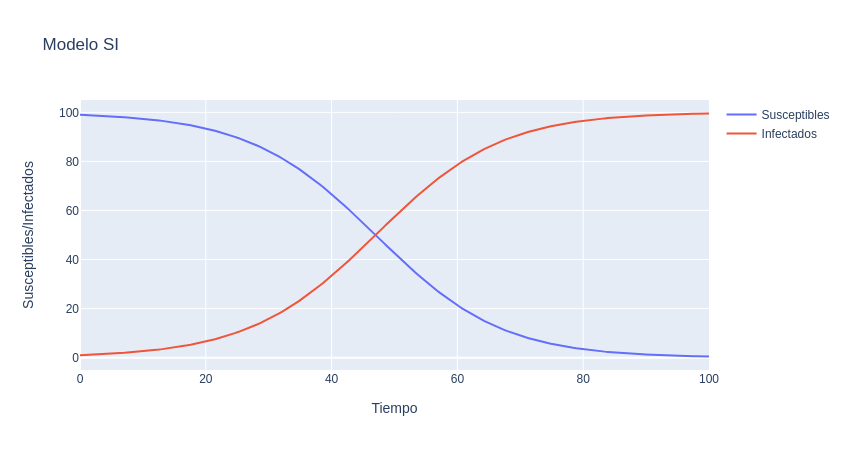
\includegraphics[scale=0.5]{SI_continuo_modelo}
\end{center}
\end{figure}

Esta ecuación diferencial se puede resolver por separación de variables como sigue:

\begin{equation}
\begin{aligned}
I'=\frac{\alpha}{N}I(N-I) & \Leftrightarrow \int \frac{dI}{I(N-I)} = \int \frac{\alpha}{N} dt \\
& \Leftrightarrow \frac{1}{N}\int \left(\frac{1}{I}+\frac{1}{N-I}\right) dI = \frac{\alpha}{N}t+c \\
& \Leftrightarrow  \frac{1}{N}\log{\frac{I}{N-I}} = \frac{\alpha}{N}t+c \\
& \Leftrightarrow  \frac{I}{N-I} = Ae^{\alpha t} \\
& \Leftrightarrow  I = Ae^{\alpha t}(N-I) \\
& \Leftrightarrow  I(1+Ae^{\alpha t}) = Ae^{\alpha t}N \\
& \Leftrightarrow  I(t) = \frac{Ae^{\alpha t}N}{1+Ae^{\alpha t} }
\end{aligned}
\end{equation}

Usando el valor inicial $I(0)=I_0$ tenemos:

\begin{equation}
\begin{aligned}
I_0 = I(0) = \frac{AN}{1+A} & \Leftrightarrow (1+A)I_0 = AN \\
& \Leftrightarrow A(N-I_0) = I_0 \\
& \Leftrightarrow A = \frac{I_0}{N-I_0}
\end {aligned}
\end{equation}

luego la solución general es:

$$I(t) = \frac{I_0e^{\alpha t}N}{(N-I_0)+I_0e^{\alpha t}} = \frac{I_0N}{(N-I_0)e^{-\alpha t}+I_0}.$$

Es claro que $I$ tiende monótonamente a $N$, luego tiene el mismo comportamiento que el modelo discreto.

En la figura \ref{fig: SI_continuo} mostramos la representación gráfica del comportamiento del modelo SI continuo. Podemos comprobar que su comportamiento es análogo al modelo discreto. También es claro que se cumple que $I$ es siempre creciente y tiende a $N$, mientras $S$ es decreciente y tiende a $0$.

\section{Modelo SIS continuo}

El modelo continuo correspondiente al modelo SIS se comporta de la misma forma que el modelo discreto, y viene expresado por:

\begin{equation}
\label{eqn: modelo_SIS_continuo}
\begin{aligned}
S'(t) = & -\frac{\alpha}{N}SI+\gamma I \\
I'(t) = & I\left( \frac{\alpha}{N}S-\gamma \right) \\
\end{aligned}
\end{equation}

donde $S(0)+I(0)=N$. En este caso el número básico reproductivo se define como $\mathcal{R}_{SIS}=\frac{\alpha}{\gamma}$.

Si $\mathcal{R}_{SIS}\leq 1$ entonces no se considera que haya una epidemia, y si $\mathcal{R}_{SIS} > 1$ hay una epidemia.

\begin{figure}
\begin{center}
\caption{Gráfica del modelo SIS continuo, en una población total de $100$ individuos, con valores iniciales $S(0)=95, I(0) = 5, \alpha = 0.1, \gamma = 0.01, T_0 = 0, T = 150$.}
\label{fig: SIS_continuo}
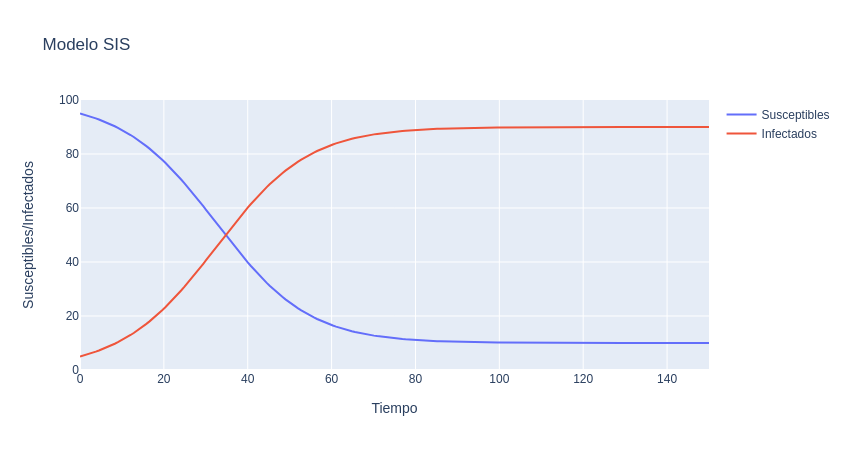
\includegraphics[scale=0.5]{SIS_continuo_modelo}
\end{center}
\end{figure}

En la figura \ref{fig: SIS_continuo} comprobamos, al igual que hicimos antes, que su comportamiento es análogo al modelo discreto. También se observa que al igual que en el modelo SI el número de individuos susceptibles es decreciente y tiende a $0$ y el de infectados creciente y tiende a $N$, pero esto no siempre es así y se debe a los parámetros usados.

\begin{figure}
\begin{center}
\caption{Gráfica del modelo SIS continuo, en una población total de $100$ individuos, con valores iniciales $S(0)=95, I(0) = 5, \alpha = 0.1, \gamma = 0.05, T_0 = 0, T = 150$.}
\label{fig: SIS_continuo2}
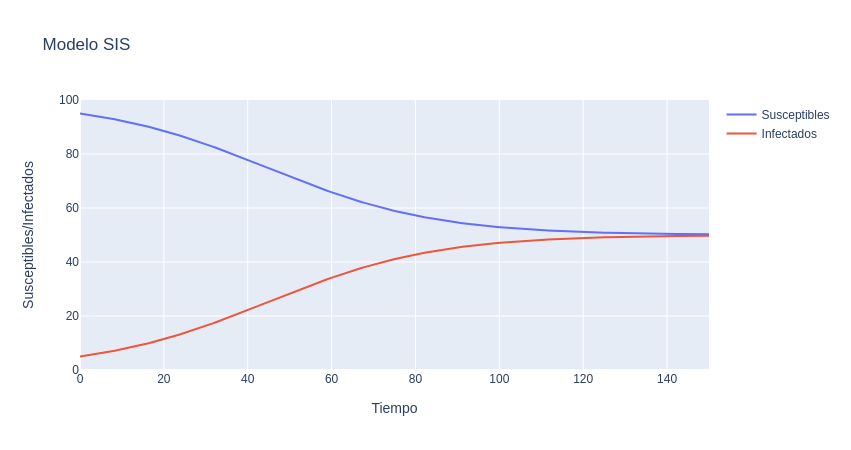
\includegraphics[scale=0.5]{SIS_continuo_modelo2}
\end{center}
\end{figure}


Por ejemplo, en la figura \ref{fig: SIS_continuo2} vemos como variando solamente $\gamma$ el modelo se comporta de forma muy diferente, pues los susceptibles e infectados parecen estabilizarse en torno a la mitad de la población.

Por otro lado, si $\gamma > \alpha$ entonces tenemos que no se produce una epidemia, pues los infectados tienden a $0$ y los susceptibles a $N$, como puede verse en la figura \ref{fig: SIS_continuo3}.

\begin{figure}
\begin{center}
\caption{Gráfica del modelo SIS continuo, en una población total de $100$ individuos, con valores iniciales $S(0)=95, I(0) = 5, \alpha = 0.1, \gamma = 0.2, T_0 = 0, T = 150$.}
\label{fig: SIS_continuo3}
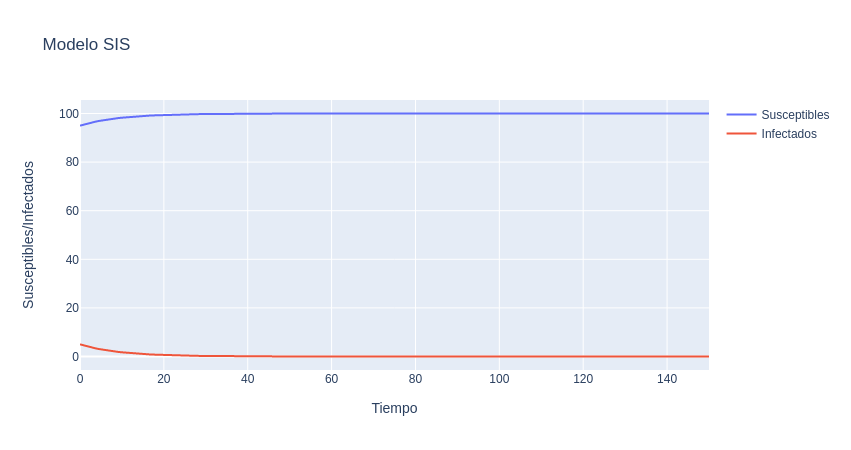
\includegraphics[scale=0.5]{SIS_continuo_modelo3}
\end{center}
\end{figure}


\section{Modelo SIR continuo}


El modelo continuo correspondiente al modelo SIR se comporta de la misma forma que el modelo discreto, y viene expresado por:

\begin{equation}
\label{eqn: modelo_SIR_continuo}
\begin{aligned}
S'(t) = & -\dfrac{\alpha}{N}SI \\
I'(t) = & I\left(\dfrac{\alpha}{N}S-\gamma \right) \\
R'(t) = & \gamma I
\end{aligned}
\end{equation}

donde $S(0)+I(0)+R(0)=N$. El número básico reproductivo en este caso se define como
$$\mathcal{R}_{SIR}=\frac{S(0)\alpha }{N\gamma },$$
y si como hemos visto $\mathcal{R}_{SIR}\leq 1$  se dice que no hay epidemia, pero en cambio, si es mayor que $1$, se dice que sí la hay.

\begin{figure}
\begin{center}
\caption{Gráfica del modelo SIR continuo, en una población total de $100$ individuos, con valores iniciales $S(0)=99, I(0) = 1, \alpha = 0.1, \gamma = 0.01, T_0 = 0, T = 300$.}
\label{fig: SIR_continuo}
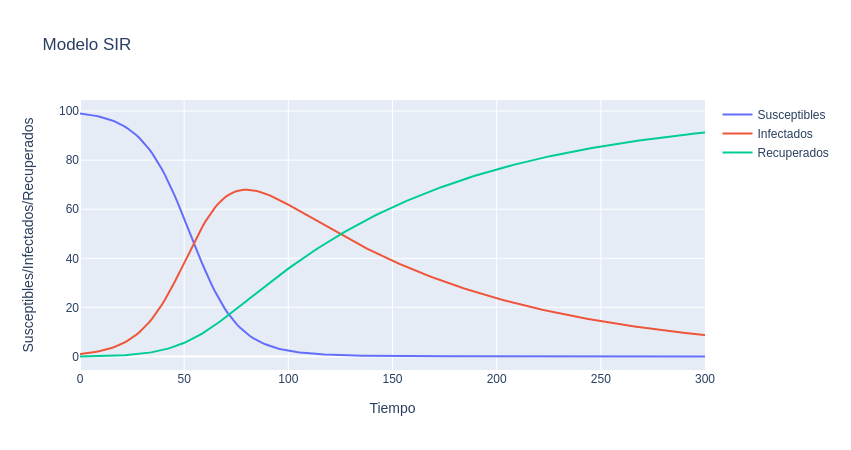
\includegraphics[scale=0.5]{SIR_continuo_modelo}
\end{center}
\end{figure}

En la figura \ref{fig: SIR_continuo} observamos el comportamiento del modelo SIR representado. Al igual que en su análogo discreto, el número de individuos susceptibles siempre decreciente y el de recuperados siempre es creciente.

\section{Modelo Kermack-McKendrick}

La información para el desarrollo de esta sección se ha obtenido principalmente de \cite{brauerMathematicalModelsPopulation2012}.

El modelo clásico de Kermack-McKendrick es un modelo sencillo basado en suposiciones simples en el flujo de la población de unos grupos a otros según su estado respecto a la enfermedad. Estos grupos son susceptibles, infectados y recuperados, inmunizados o fallecidos.

Este modelo es, por tanto, una modificación del modelo SIR. La diferencia con el modelo SIR ya estudiado es que en este modelo se supone que un individuo infectado hace contacto suficiente para contagiar la enfermedad con $\alpha N$ individuos por unidad de tiempo, mientras en el modelo SIR se supone que $\alpha$ es el número medio de individuos con los que un infectado tiene suficiente contacto para contagiarlo en una unidad de tiempo. Por tanto, en este apartado y para hacer notar esta diferencia usaremos $\bar{\alpha}$ en lugar de $\alpha$.

El modelo se describe como:

\begin{equation}
\label{eqn: KMK}
\begin{aligned}
S' & = -\bar{\alpha} SI \\
I' & = \bar{\alpha} SI - \gamma I \\
R' & = \gamma I
\end{aligned}
\end{equation}

Las suposiciones en las que se basa el modelo descrito son:

\begin{itemize}
\item Un individuo hace contacto suficiente para contagiar la enfermedad con $\bar{\alpha} N$ individuos por unidad de tiempo, siendo $N$ el total de la población.
\item Los infectados pasan a recuperados, inmunizados o fallecidos con la tasa $\gamma I$ por unidad de tiempo.
\item La población total es constante, no hay incorporaciones ni salidas.
\item No se consideran los fallecimientos como grupo aparte, así la población es constante.
\end{itemize}

\begin{figure}
\begin{center}
\caption{Esquema del modelo de Kermack-McKendrick y modelo SIR}
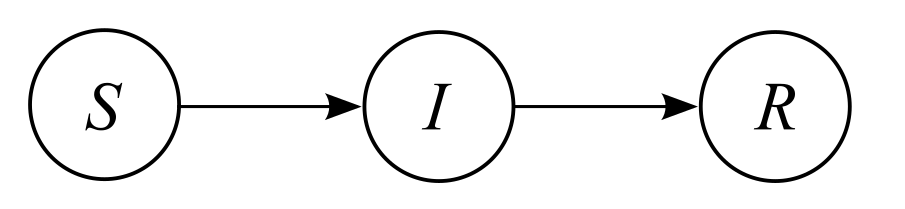
\includegraphics[scale=0.5]{esquema_sir}
\end{center}
\end{figure}

De acuerdo con la primera suposición, dado que la probabilidad de que aleatoriamente el contacto de un infectado sea con un individuo susceptible es $\frac{S}{N}$, el número de nuevos infectados por unidad de tiempo por infectado es $\frac{\bar{\alpha} NS}{N}$, dando lugar a una tasa de nuevos infectados de $\frac{\bar{\alpha}  N S I}{N}=\bar{\alpha} SI$. Notemos que ambas aproximaciones dan lugar a la misma tasa de nuevos infectados.

Observemos también que, al igual que en el modelo SIR, se cumple $N=S+I+R$.

Para la tercera suposición consideramos el grupo de individuos que fueron infectados en un mismo momento, y sea $u(s)$ el conjunto de estos que aún son infecciosos $s$ unidades de tiempo después de haber sido infectados. Si una porción $\gamma$ de estos deja de pertenecer a la clase de individuos infectados por unidad de tiempo, entonces

$$u'=-\gamma u,$$

y la solución de esta ecuación diferencial es

$$u(s)=u(0)e^{-\gamma s}.$$

Por tanto, la fracción de infectados que siguen estando en la clase infectados $s$ unidades de tiempo después de haberse convertido en infectados es $e^{-\gamma s}$, luego la duración del período infeccioso se distribuye según una exponencial, con significado
$$\int_0^\infty e^{-\gamma s}ds=1/\gamma,$$
y esto es lo que la segunda suposición realmente significa. Si en lugar de suponer esto, suponemos que la fracción de infectados que permanecen infectados en un tiempo $\tau$ después de haberse infectado es $P(\tau )$, la segunda ecuación de \eqref{eqn: KMK} se reemplaza por:

$$I(t)=I_0(t)+\int_0^\infty \bar{\alpha} S(t-\tau )I(t-\tau )P(\tau ) d\tau ,$$

donde $I_0(t)$ hace referencia a los miembros de la población que estaban infectados en el instante inicial y siguen siendo infecciosos en el momento $t$.

Las suposiciones de que la tasa de contactos es proporcional al tamaño de la población $N$ con una constante de proporcionalidad constante $\bar{\alpha}$ y de una distribución exponencial de tasa de recuperación son demasiado simples para ser realistas. Existen otros modelos más generales que se pueden analizar, pero finalmente muchos modelos más realistas muestran comportamientos similares a estos modelos más simples.

En nuestro modelo \eqref{eqn: KMK}, $R$ se determina una vez que se conocen $S$ e $I$, pero podemos eliminar la tercera ecuación del modelo, dejando este formado solamente por dos ecuaciones:

\begin{equation}
\label{eqn: KMK_sinR}
\begin{aligned}
S' & = -\bar{\alpha} SI, \\
I' & = (\bar{\alpha} S - \gamma ) I,
\end{aligned}
\end{equation}

junto con las condiciones iniciales:
$$S(0)=S_0, \quad I(0)=I_0, \quad S_0+I_0=N.$$

El modelo solo tiene sentido si $S(t)$ e $I(t)$ se mantienen no negativos, luego si alguno de los dos llega a $0$, consideramos que el estudio ha terminado.

\begin{lemma}
Dado el modelo \eqref{eqn: KMK_sinR}, se tiene que $S'<0$ para todo $t$, y además $I'>0$ si, y solo si, $S>\frac{\gamma}{\bar{\alpha}}$.
\end{lemma}

Es decir, $I$ aumenta mientras se cumpla que $S>\frac{\gamma}{\bar{\alpha}}$, pero como $S$ decrece para todo $t$, finalmente se tiene que $S<\frac{\gamma}{\bar{\alpha}}$, y por tanto $I$ deja de aumentar.

Si $S_0<\frac{\gamma}{\bar{\alpha}}$, entonces $I$ decrece a $0$ y no hay una epidemia, mientras que si $S_0>\frac{\gamma}{\bar{\alpha}}$, $I$ comienza creciendo hasta el máximo obtenido cuando $S=\frac{\gamma}{\bar{\alpha}}$ y luego decrece hasta $0$, en cuyo caso hay una epidemia.

Definimos el número básico reproductivo como:

$$\mathcal{R}_{KMK}=\frac{\bar{\alpha} S_0}{\gamma}.$$

De esta manera, si $\mathcal{R}_{KMK}\leq 1$ no hay una epidemia, mientras si $\mathcal{R}_{KMK}>1$ hay una epidemia. 





\section{Análisis de los parámetros de los modelos}

Estimar la tasa de transmisión media es uno de los aspectos más cruciales en epidemiología. Esta tasa condiciona la fase de la epidemia e incluso si va a extinguirse. Es combinación de tres factores:

\begin{enumerate}
\item Coeficiente de virulencia: Relacionado con el agente infeccioso.
\item Coeficiente de susceptibilidad: Relacionado con el anfitrión.
\item Número de contactos por unidad de tiempo entre individuos.
\end{enumerate}

Los dos primeros factores se tienen en cuenta a la vez en la probabilidad de transmisión.

Todos los factores pueden cambiar con el tiempo. El primero, debido a mutaciones del virus y los dos últimos por medidas de contención. Por tanto, observar el decrecimiento de la transmisión media en una enfermedad es una buena forma de comprobar la efectividad de las medidas de contención.

En el artículo \cite{demongeotSIEpidemicModel} se presenta un modelo SI modificado con el objetivo de compararlo con los datos obtenidos en la pandemia de la Covid-19 en China hasta el momento, y así tratar de predecir su comportamiento en el futuro.

El modelo SI continuo considerado es el siguiente:

\begin{equation}
\label{eqn: SI_cont}
\begin{aligned}
S'(t) = & -\tau (t)S(t)I(t) \\
I'(t) = & \tau (t)S(t)I(t) -vI(t)
\end{aligned}
\end{equation}

donde $S(t)$ es el número de individuos susceptibles , $I(t)$ el número de individuos infectados en el tiempo $t$ y $\tau (t)$ la tasa de transmisión, que combina el número de contactos por unidad de tiempo y la probabilidad de transmisión. Observemos que $\tau (t)$ se considera variable respecto al tiempo, al contrario que en el caso SI clásico estudiado antes. Además, notemos que $v$ es una constante, donde $1/v$ es la duración media del período de infección, y $vI(t)$ el flujo de individuos recuperados o fallecidos. %vI(t) es el flujo de recuperados o muertos porque ha mezclado el modelo SI y SIR; vI(t) serian los recuperados, pero se ahorra la ecuacion de la R

Se consideran las condiciones iniciales

$$S(t_0)=S_0>0, \: I(t_0)=I_0>0.$$

Siguiendo \cite{demongeotSIEpidemicModel}, ahora consideramos que al final del período infeccioso nos han informado de una fracción del total de casos, en este caso la fracción la denotamos por $f\in (0,1]$. Sea $C_R(t)$ el número total acumulado de casos reportados. Entonces:

\begin{equation}
\label{eqn: acumulada}
C_R(t) = {C_R}_0 + vfC_I(t), \forall t \geq t_0
\end{equation}

donde $C_{R0}$ representa el número de casos reportados al inicio del estudio y 

$$C_I(t) = \int_{t_0}^t I(w) dw $$

siendo $C_I$ el número total de infectados acumulado.

Asumimos conocidos $S_0 > 0$, $1/v>0$, $f\in (0,1]$. Por tanto, queremos averiguar el número inicial de infectados $I_0$ y la tasa de transmisión $\tau (t)$.

\subsection{Aproximación de $I_0$ y $\tau (t_0)$}
Siguiendo \cite{demongeotSIEpidemicModel}, procedemos a intentar aproximar $I_0$ y $\tau (t_0)$:

Al comienzo de la pandemia podemos suponer que $S(t)$ y $\tau (t)$ son constantes e iguales a $S_0$ y $\tau_0 = \tau (t_0)$, respectivamente. Sustituyendo estos valores en la ecuación \eqref{eqn: SI_cont} obtenemos:

$$I'(t) = (\tau_0 S_0 -v) I(t).$$

Resolviendo la ecuación diferencial llegamos a:

$$I(t) = I_0\exp{((\tau_0 S_0-v)(t-t_0))},$$

y sustituyendo en \eqref{eqn: acumulada}:

$$C_R(t) = {C_R}_0 + vfI_0\frac{\mathrm{e}^{(\tau_0 S_0 -v)(t-t_0)} -1}{\tau_0 S_0-v}.$$

De este modo, hemos obtenido un primer modelo para los casos acumulados al principio de la pandemia.

Reescribimos la ecuación anterior como:

\begin{equation}
\label{eqn: acumulada_modelo}
C_R(t) = \chi_1 \mathrm{e}^{\chi_2 t} -\chi_3.
\end{equation}

Estimamos $\chi_3$ usando los datos de la epidemia obtenidos, y el mejor ajuste para los datos se obtiene con $\chi_3=0$.

Ahora, usando \eqref{eqn: acumulada} y \eqref{eqn: acumulada_modelo} tenemos:

\begin{equation}
I_0=\frac{\chi_1\chi_2\mathrm{e}^{\chi_2 t_0}}{vf}
\end{equation}

Y, como sabemos que $\chi_2 = \tau_0 S_0-v$, entonces

\begin{equation}
\tau_0 = \frac{\chi_2+v}{S_0}.
\end{equation}

Si suponemos $\tau (t) = \tau_0$ constante, tenemos que el modelo queda:

\begin{equation}
\begin{aligned}
S'(t) = -\tau_0S(t)I(t) \\
I'(t) = \tau_0S(t)I(t) -vI(t)
\end{aligned}
\end{equation}

Usando la ecuación de $S(t)$ y resolviéndola obtenemos:

$$S(t) = S_0\exp{\left( -\tau_0 \int_{t_0}^t I(w) dw \right)} = S_0\exp{(-\tau_0 C_I(t))}.$$

Ahora, sustituyendo esta expresión en la ecuación de $I(t)$ del modelo y usando $C_I'(t)=I(t)$:

$$I'(t) = S_0\exp{\left( -\tau_0 C_I(t)\right) }\tau_0 C_I'(t)-vI(t).$$

Finalmente, integrando entre $t_0$ y $t$ tenemos que:

$$I(t)=C_I'(t)=I_0+S_0(1-\exp{(-\tau_0 C_I(t)}))-vC_I(t).$$
 
Observamos entonces que el número total acumulado de infectados es monótono creciente, ya que $I(t)>0$ siempre por positividad de las soluciones y $C_I'(t)=I(t)>0$. Cabe destacar que esto no implica que el número de infectados sea monótono creciente.

\begin{theorem}
Sea $t>t_0$ fijo. El número de infectados acumulados es estrictamente creciente respecto a las siguiente cantidades:
\begin{itemize}
\item $I_0>0$: Número inicial de infectados
\item $S_0>0$: Número inicial de individuos susceptibles.
\item $\tau>0$: Tasa de transmisión
\item $1/v$: Tiempo medio de la infección.
\end{itemize}
\end{theorem}

\subsection{Fórmula teórica para $\tau (t)$}

Usando la ecuación del modelo inicial \eqref{eqn: SI_cont} obtenemos:
% La ecuacion de la S$

$$S(t) = S_0 \exp{\left( - \int_{t_0}^t \tau(w) I(w) dw \right) } $$ 

Ahora, sustituyendo en la ecuación \eqref{eqn: SI_cont}:
% La ecuacion de la I

$$I'(t) = S_0 \exp{\left( - \int_{t_0}^t \tau(w) I(w) dw \right) } \tau (t) I(t) -vI(t) $$

Integramos en ambos lados entre $t_0$ y $t$, luego:

$$ C_I'(t) = I_0 + S_0 \left( 1-\exp{\left(- \int_{t_0}^t \tau (w) I(w)dw \right)}\right) -vC_I(t)$$

Equivalentemente, por \eqref{eqn: acumulada}:

$$C_R'(t) = vf\left( I_0 + S_0 \left( 1-\exp{\left(- \frac{1}{vf}\int_{t_0}^t \tau (w ) C_R'(w)dw \right)}\right)\right) +v{C_R}_0 -vC_R(t)$$

Así, obtenemos el Teorema 3.1 de \cite{demongeotSIEpidemicModel}, que nos da la relación directa buscada.









%\ctparttext{\color{black}\begin{center}
%		Esta es una descripción de la parte de informática.
%\end{center}}

%\part{Parte de informática}
\chapter{Desarrollo del software: Análisis y diseño}

\section{Objetivos y análisis de requisitos}

Los objetivos que se persiguen al realizar este proyecto son realizar un estudio de distintos modelos de epidemiología. Se pretende comprender cómo afectan sus parámetros y condiciones iniciales a la evolución en el tiempo de estos modelos desde un punto de vista tanto teórico como práctico, apoyándonos en distintas gráficas interactivas para ilustrar dichos comportamientos. Asimismo, se va a analizar la bondad de ajustes de parámetros de algunos de los modelos presentados aplicados a datos reales comprobando cuáles proporcionan mejores resultados en cada caso. Con el fin de satisfacer todos estos objetivos, se ha extraído la siguiente lista de requisitos:

\begin{itemize}
\item \textbf{Requisitos funcionales}
	\begin{itemize}
	\item \textbf{RF1}: Se debe poder modificar los parámetros de las gráficas de los distintos modelos.
	\item \textbf{RF2}: El usuario debe poder elegir con qué modelo quiere trabajar.
	\item \textbf{RF3}: El sistema debe permitir descargar las imágenes de las gráficas obtenidas.
	\item \textbf{RF4}: El sistema debe poder cargar y leer ficheros de datos.
	\item \textbf{RF5}: Se debe visualizar el ajuste obtenido mediante gráficas.
	\item \textbf{RF6}: Para cada ajuste realizado se obtendrá los valores estimados de los parámetros y los errores.
	\item \textbf{RF7}: El sistema debe ser capaz de seleccionar qué modelo se ajusta mejor a los datos. 
	\end{itemize}
\item \textbf{Requisitos no funcionales}
	\begin{itemize}
	\item \textbf{RNF1}: No se podrán ajustar datos de más de un fichero a la vez.
	\item \textbf{RNF2}: Las gráficas deben actualizarse en tiempo real.
	\item \textbf{RNF3}: Se mostrará información de ayuda, en caso de ser necesaria.
	\item \textbf{RNF4}: Se debe poder usar desde el navegador.
	\end{itemize}
\item \textbf{Requisitos de información}
	\begin{itemize}
	\item \textbf{RI1}: Los ficheros de datos con los que se va a trabajar deben ser formato csv con una estructura específica, dependiente de cada modelo.
	\end{itemize}
\end{itemize}

\section{Desarrollo del proyecto}

Actualmente hay diversas metodologías de desarrollo del software. Cada uno de estos modelos consta de una serie de etapas en las que se ha dividido el desarrollo. Para este proyecto, se ha optado por el modelo en espiral. En este modelo el software se desarrolla de forma incremental, es decir, se van añadiendo funcionalidades y mejoras al software según se van evaluando las que ya tiene. Cada bucle o iteración representa un conjunto de actividades. Estas actividades no están fijadas a ninguna prioridad, sino que las siguientes se eligen en función del análisis de riesgo, comenzando por el bucle interior, como se describe en la figura \eqref{modelo_espiral}.

\begin{figure}
\begin{center}
\caption{Modelo en espiral.}
\label{modelo_espiral}
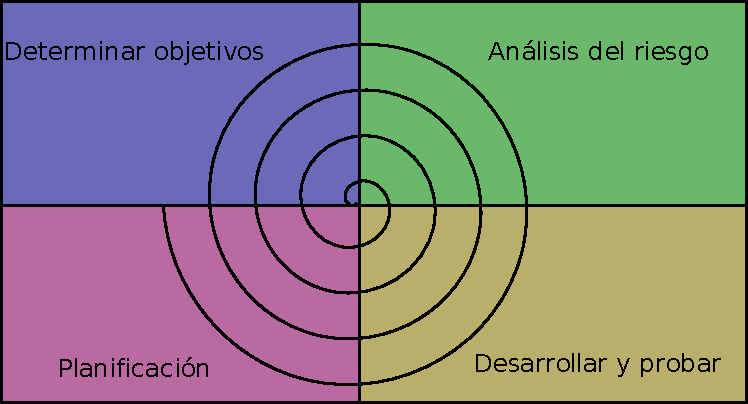
\includegraphics[scale=1]{modelo_espiral}
\end{center}
\end{figure}

Se ha elegido este método de desarrollo ya que se consigue un desarrollo muy estable, pues toda funcionalidad añadida al software es probada y evaluada. De esta forma, aunque el proyecto no esté completo, siempre se tiene una parte funcional, y se va incrementando de forma que siempre disponemos de un producto mínimamente viable. 

\section{Gestión de recursos}

Los proyectos que se pueden realizar dependen en gran medida de los recursos que se pueden destinar a ellos. Se requieren unos elementos mínimos que son indispensables para poder llevarlo a cabo. Por ello, es muy importante contar con los recursos necesarios y gestionarlos de manera adecuada.

\subsection{Recursos humanos}

El proyecto consta de un equipo de 3 personas para llevarlo a cabo:

\begin{itemize}
\item Ana Buendía Ruiz-Azuaga, se encarga de:
	\begin{itemize}
	\item Planificación y análisis del proyecto.
	\item Búsqueda de bibliografía.
	\item Diseño e implementación del proyecto.
	\item Pruebas para el correcto funcionamiento del proyecto.
	\item Redacción de la documentación del proyecto.
	\end{itemize}
\item Tutores: Manuel Pegalajar Cuéllar y Teresa E. Pérez, encargados de:
	\begin{itemize}
	\item Idea original del proyecto.
	\item Proporcionar bibliografía.
	\item Guiar para la redacción de la memoria y documentación.
	\item Supervisar el desarrollo del proyecto.
	\end{itemize}
\end{itemize}

\subsection{Recursos hardware}

Todo el proyecto se va a desarrollar en un ordenador portátil con todo el software y dependencias necesarias. Las especificaciones del portátil son:

\begin{itemize}
\item \textbf{Modelo}: Acer Aspire E-5 574G.
\item \textbf{CPU}: Intel Core i5-6200U.
\item \textbf{RAM} 8GB RAM DDR3.
\item \textbf{Disco duro}: 1TB.
\item \textbf{Precio}: 600€.
\end{itemize}

\subsection{Recursos software}

El proyecto se ha llevado a cabo usando como sistema operativo Ubuntu 20.04 LTS, y se ha usado como lenguaje principal Python.

El software necesario para el proyecto es el siguiente:

\begin{itemize}
\item \textbf{Flask}. Flask es un microframework web en python. Proporciona funcionalidad básica para, de forma sencilla, crear una aplicación web. Una posible alternativa habría sido Django, pero finalmente se ha optado por Flask debido a su simplicidad, legibilidad y que en este proyecto no se requieren muchas de las funcionalidades que Django ofrece integradas. 
\item \textbf{Dash}. Dash es un framework opensource basado en plotly.js y react.js que permite crear fácilmente aplicaciones basadas en datos. En este proyecto se ha usado principalmente por su capacidad de crear gráficas interactivas en tiempo real. 
\item \textbf{VSCode}. Se ha usado VSCode como editor de texto, ya que proporciona una gran cantidad de plugins para cualquier lenguaje, así como integración con git.
\item \textbf{Draw.io}. Para la realización de diagramas de distintas clases, se ha usado el software de dibujo gratuito Draw.io.
\item \textbf{Docker}. Con el fin de simplificar el lanzamiento y ejecución de la aplicación web desarrollada se ha usado docker para virtualizar el entorno y evitar la necesidad de instalar en cualquier máquina el software necesario para ejecutarla.
\item \textbf{Git}. Se ha empleado Git como controlador de versiones, integrado con Github.
\item \textbf{Texmaker}. Para redactar la memoria, se ha usado el editor de LaTeX Texmaker.
\end{itemize}

Todo el software utilizado ha sido gratuito, por lo que no ha tenido coste alguno.

\subsection{Estimación del coste}

A partir de los recursos previamente listados, se va a realizar una aproximación del coste de la consecución del proyecto, considerando que la duración del mismo es de 9 meses.

Para los recursos humanos, dado que se considera que la alumna ha trabajado aproximadamente 450 horas de acuerdo a los créditos correspondientes asignados al TFG, y el gasto aproximado es 15€/h en calidad de alumna de prácticas, se tiene que el coste es de 6.750,00€.

A los tutores, dada su formación profesional se les supone un coste estimado de 50€/h, y aproximando que se dedican 3 horas semanales para la tutorización del proyecto, se tiene que el coste total tras los 9 meses es de 5.400,00€ por tutor.

Dado que el portátil empleado tiene una vida útil estimada de 5 años, le corresponde un coste de 120,00€ durante la realización del proyecto.

Finalmente, dado que todo el software empleado es gratuito, el coste aproximado del proyecto aparece desglosado en la tabla \eqref{tabla_pres}.

\begin{table}[!h]
\caption{Desglose de presupuesto del proyecto.}
\begin{center}
\begin{tabular}{|c c|} 
 \hline
 \textbf{Recursos humanos} & \textbf{Coste (€)} \\ 
 \hline\hline
 Alumna & 6.750,00 \\
 \hline
 Tutor 1 & 5.400,00 \\
 \hline 
 Tutor 2 & 5.400,00 \\
 \textbf{Suma} & \textbf{17.550,00} \\
 \hline
 \textbf{Recursos hardware} & \textbf{Coste (€)} \\ 
 \hline\hline
 Ordenador portátil & 120,00 \\
 \hline
 \textbf{Suma} & \textbf{120,00} \\
 \hline 
 \textbf{Recursos software} & \textbf{Coste (€)} \\
 \hline
  Flask & 0,00 \\
  \hline
  Dash & 0,00 \\
  \hline 
  VSCode & 0,00 \\
  \hline
  TexMaker & 0,00 \\
  \hline 
  \textbf{Suma} & \textbf{0,00} \\ 
 \hline\hline
 \textbf{Suma total} & \textbf{17.670,00} \\
 \hline\hline
 \textbf{Gastos indirectos (18\%)} & \textbf{3.180,60} \\ 
 \hline\hline
 \textbf{Total} & \textbf{20.850,60} \\ 
 \hline\hline
 \textbf{IVA (21\%)} & \textbf{4.378,63} \\ % es .626 
 \hline\hline
 \textbf{Coste final} & \textbf{25.229,23} \\  % es .226
 \hline\hline

 \hline
\end{tabular}
\label{tabla_pres}
\end{center}
\end{table}

\section{Planificación temporal}

Para la realización del proyecto se han distinguido distintas etapas, y en cada una de ellas se ha implementado y trabajado sobre una funcionalidad concreta, de acuerdo al modelo en espiral. Las distintas partes del proyecto han sido:

\begin{itemize}
\item \textbf{T1. Estudio de bibliografía y estado actual de la epidemiología}. Se han consultado diversos libros, artículos y páginas de interés con el fin de comprender mejor y obtener los recursos necesarios para la realización del proyecto. Además, se ha realizado una selección de los modelos a estudiar y tratar durante el desarrollo del mismo.
\item \textbf{T2. Especificación de requisitos}. En base a la información obtenida del proyecto, en esta etapa se han especificado los requisitos que el software debe cumplir.
\item \textbf{T3. Diseño del sistema}. A partir de los requisitos especificados, se ha diseñado la arquitectura del sistema y cómo será la interfaz con la que van a interactuar los usuarios.
\item \textbf{T4. Marco teórico}. Se han indicado conceptos y modelos, así como estudiado las características de estos con el fin de desarrollar la teoría necesaria para trabajar con modelos epidemiológicos. Asimismo, se ha indicado el contexto en el que la epidemiología es de gran utilidad.
\item \textbf{T5. Implementación de los modelos discretos}. Se ha realizado la implementación de los modelos discretos SI, SIR y SIS, incluyendo gráficas interactivas de los mismos.
\item \textbf{T6. Implementación de los modelos continuos}. Se ha realizado la implementación de los modelos continuos SI, SIR y SIS, incluyendo gráficas interactivas de los mismos, al igual que información teórica.
\item \textbf{T7. Ajuste de datos a diversos modelos}. Se ha implementado una funcionalidad para realizar un ajuste de parámetros de acuerdo a un modelo a elegir, o el sistema puede determinar cuál es el modelo que minimiza el error para unos datos dados.
\item \textbf{T8. Documentación del proyecto}. Se ha llevado a cabo la documentación del proyecto durante todo su desarrollo.
\end{itemize}

Con el fin de ayudar a hacer más fácil la comprensión de cómo se ha distribuido el tiempo del proyecto, se ha realizado el diagrama \eqref{fig: planificacion} en el que se puede ver cuánto tiempo se ha dedicado a cada etapa del desarrollo del proyecto durante los 10 meses de duración del mismo.

\begin{figure}[!h]
\begin{center}
\caption{Planificación temporal de las etapas del proyecto.}
\label{fig: planificacion}
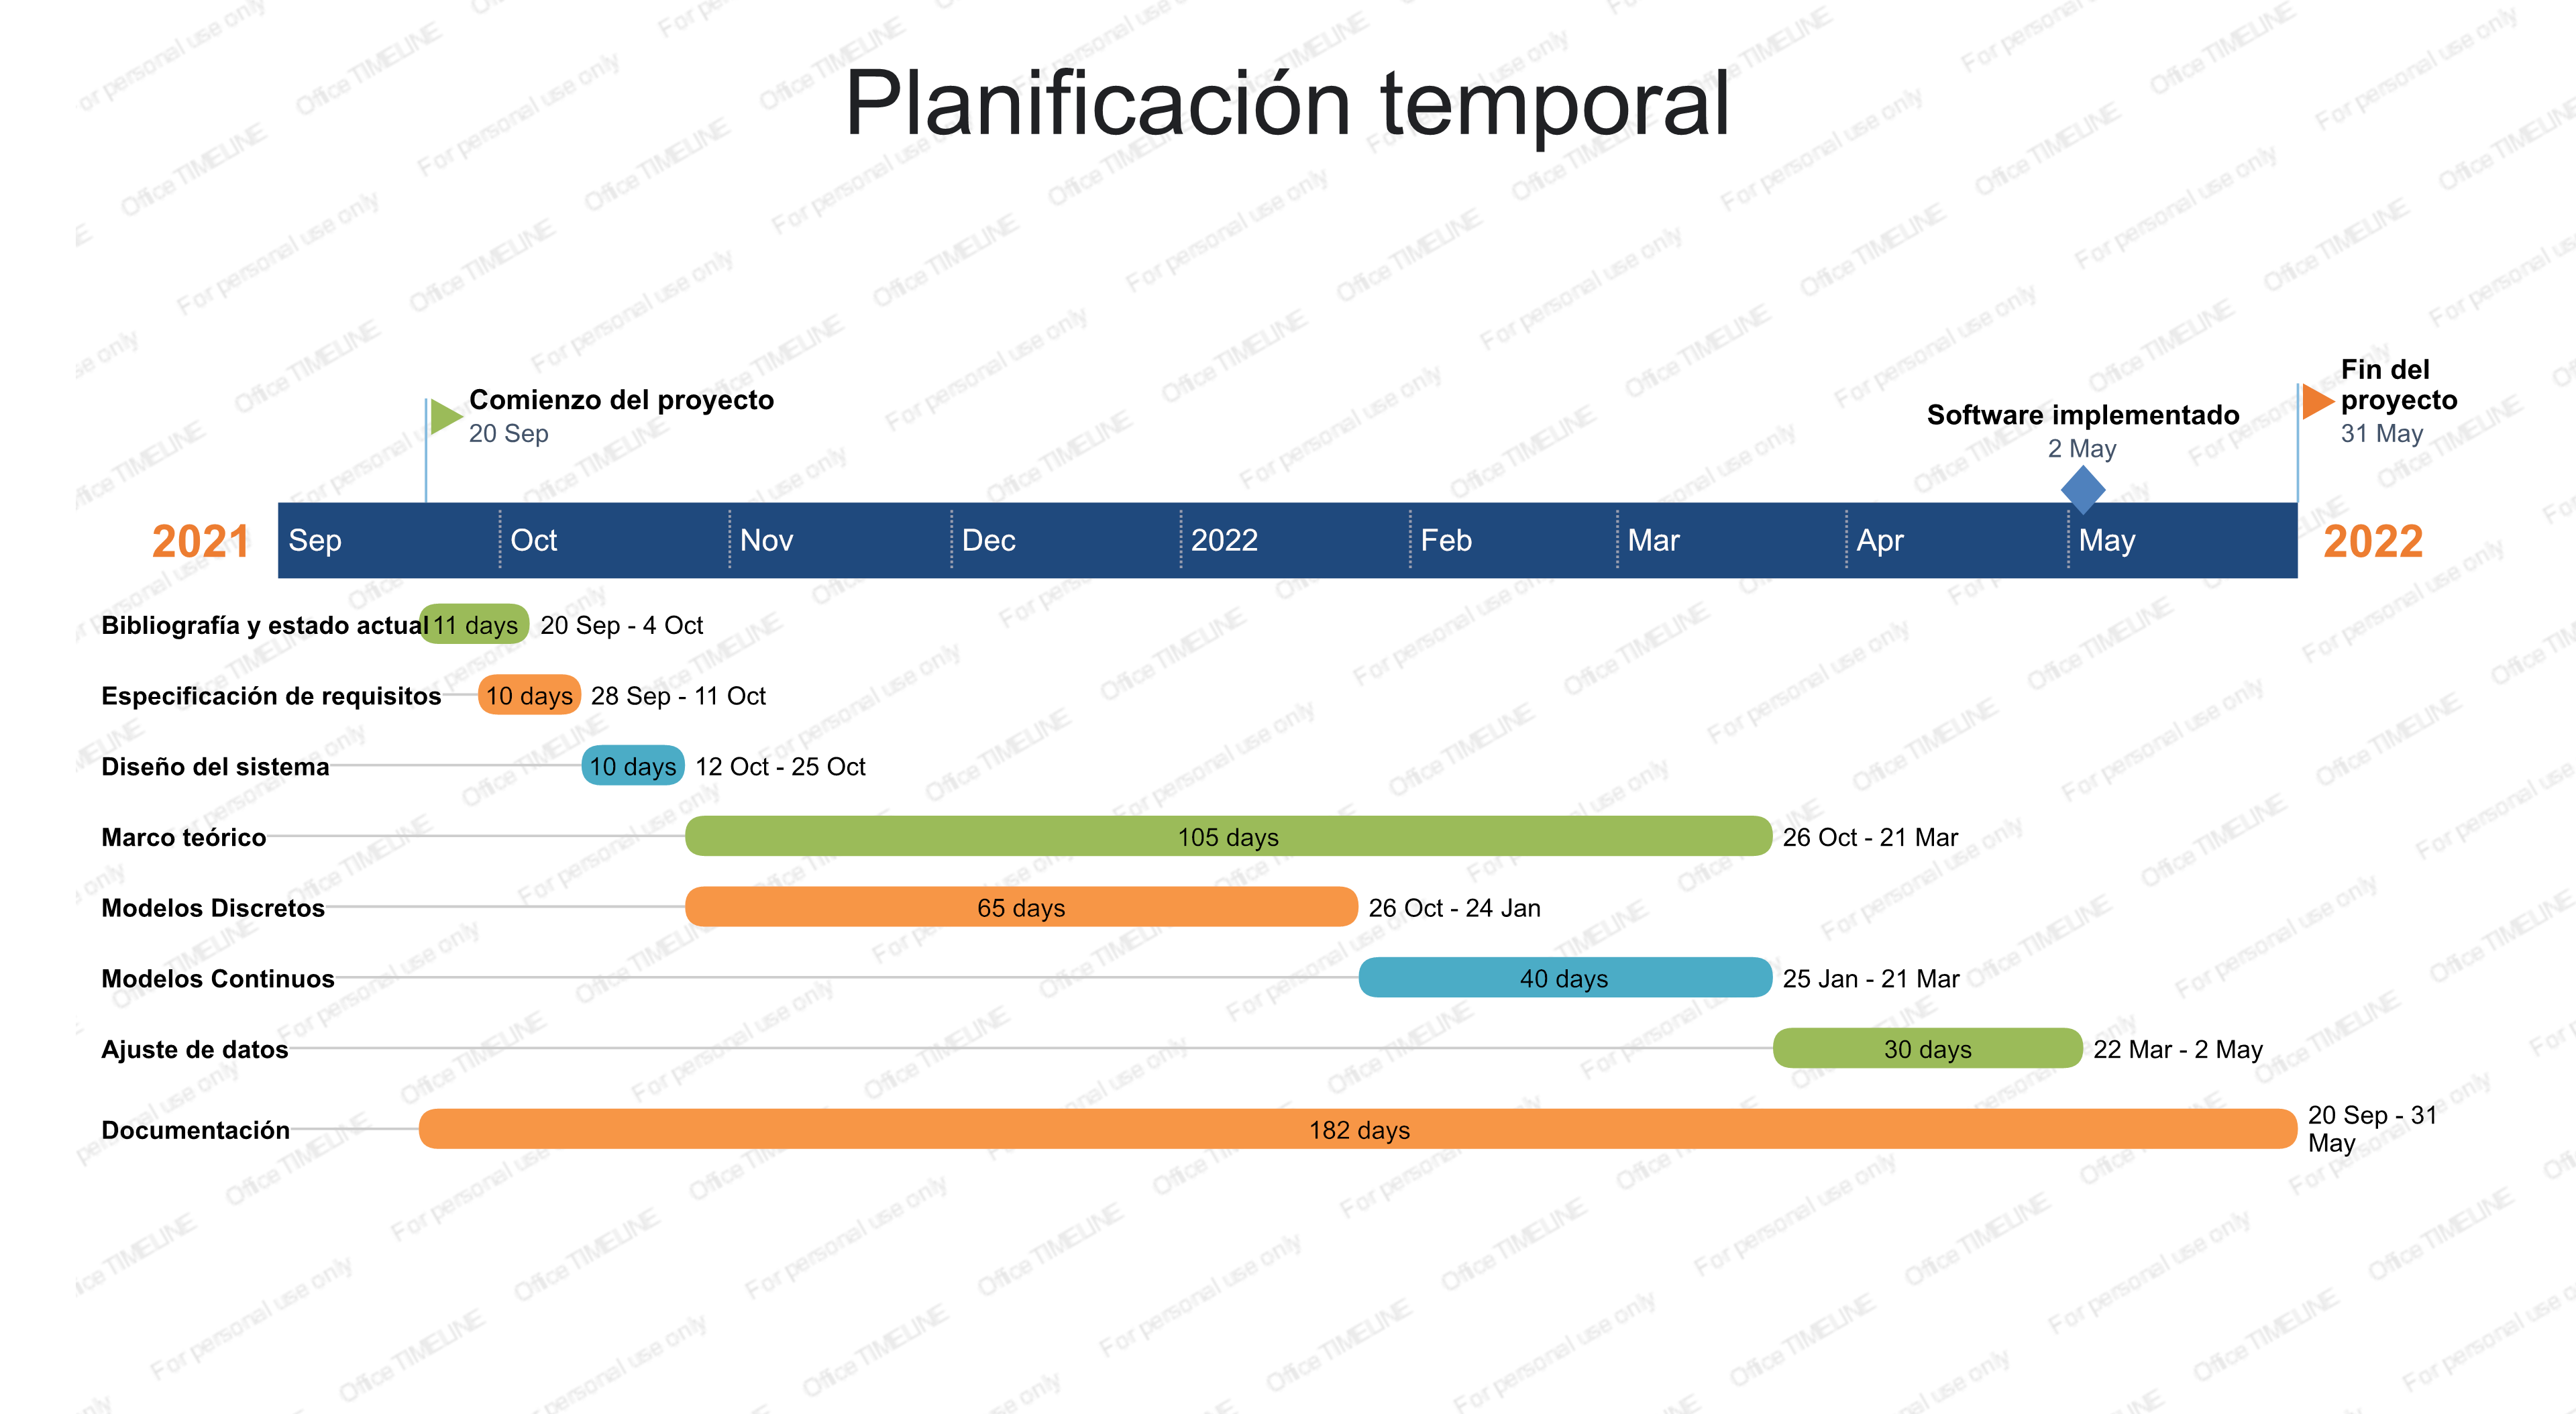
\includegraphics[scale=0.35]{planificacion}
\end{center}
\end{figure}


\section{Diagrama conceptual}

Para el modelado conceptual de la aplicación web, se ha optado por utilizar OOWS (Object-Oriented approach for Web Solutions modelling), que usa modelado de objetos UML y modelos de navegación y presentación usando UML. Así, se expresan las características navegacionales de la aplicación web a la vez que se integra con las restantes vistas del esquema conceptual mediante una notación UML adaptada.

En \eqref{diag: modelo_concep}, se muestra el diagrama conceptual, construido mediante una estrategia top-down:

\begin{figure}[!h]
\begin{center}
\caption{Modelo conceptual de la aplicación web.}
\label{diag: modelo_concep}
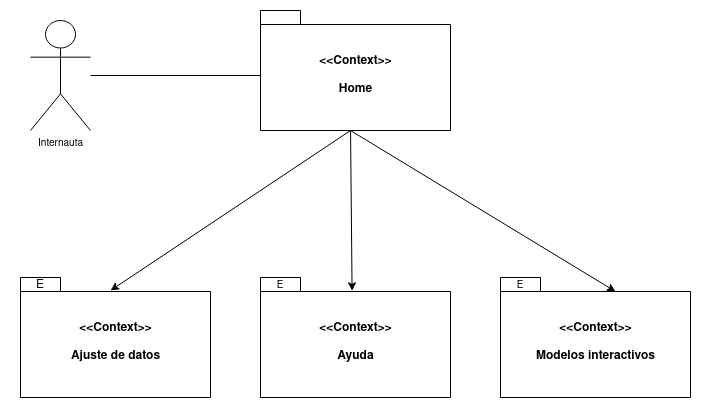
\includegraphics[scale=0.5]{modelo_conceptual-vista-paquetes.drawio}
\end{center}
\end{figure}

En \eqref{diag: modelo_concep_home} se muestra el detalle del contexto de \verb|Home|, en \eqref{diag: modelo_concep_modelos} se ve el detalle de \verb|Modelos Interactivos|, así como en \eqref{diag: modelo_concep_ayuda} el de \verb|Ayuda| y en \eqref{diag: modelo_concep_ajuste} el de \verb|Ajuste de datos|.

\begin{figure}[!h]
\begin{center}
\caption{Modelo conceptual del contexto de Inicio.}
\label{diag: modelo_concep_home}
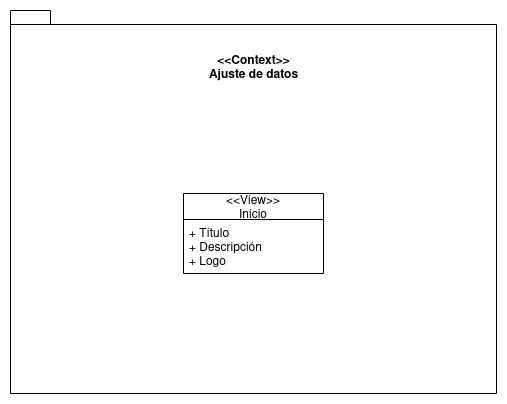
\includegraphics[scale=0.5]{modelo_conceptual-home.drawio}
\end{center}
\end{figure}

\begin{figure}[!h]
\begin{center}
\caption{Modelo conceptual del contexto de Modelos Interactivos.}
\label{diag: modelo_concep_modelos}
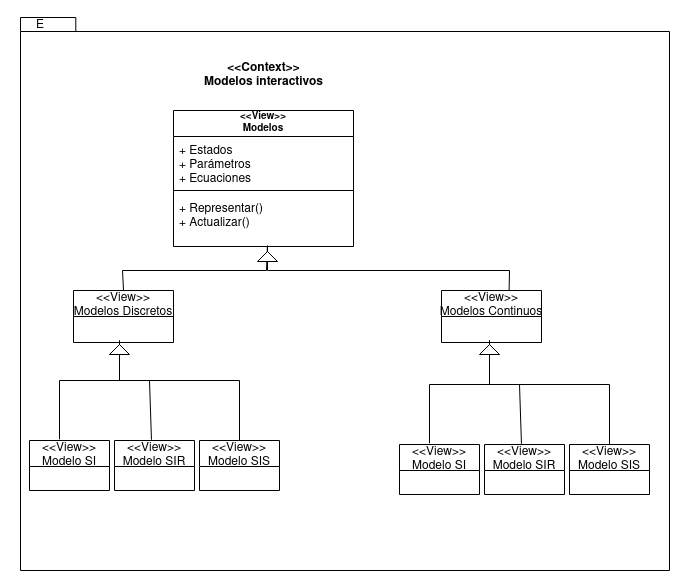
\includegraphics[scale=0.5]{modelo_conceptual-Modelos.drawio}
\end{center}
\end{figure}

\begin{figure}[!h]
\begin{center}
\caption{Modelo conceptual del contexto de Ayuda.}
\label{diag: modelo_concep_ayuda}
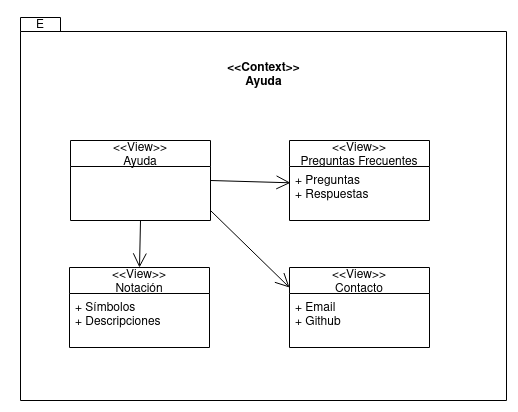
\includegraphics[scale=0.5]{modelo_conceptual-Ayuda.drawio}
\end{center}
\end{figure}

\begin{figure}[!h]
\begin{center}
\caption{Modelo conceptual del contexto de Ajuste de Datos.}
\label{diag: modelo_concep_ajuste}
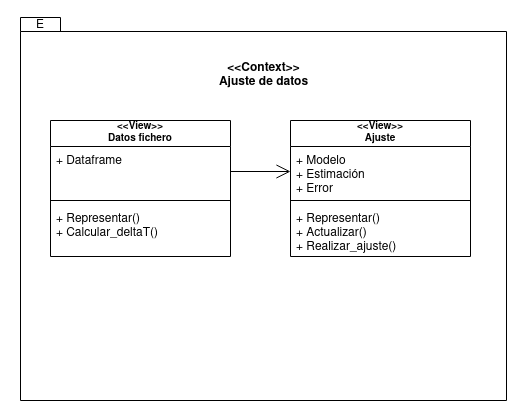
\includegraphics[scale=0.5]{modelo_conceptual-Ajuste.drawio}
\end{center}
\end{figure}





\section{Casos de uso}

A partir de los requisitos listados anteriormente, se obtienen los siguientes casos de uso:

\begin{itemize}
\item \textbf{CU-1}: Modificar parámetro de un modelo.
\item \textbf{CU-2}: Preprocesar entrada.
\item \textbf{CU-3}: Subir fichero de datos.
\item \textbf{CU-4}: Leer fichero de datos.
\item \textbf{CU-5}: Actualizar gráfica.
\item \textbf{CU-6}: Seleccionar modelo de ajuste.
\item \textbf{CU-7}: Realizar ajuste de datos.
\item \textbf{CU-8}: Descargar gráfica.
\end{itemize}

\subsection{Actores del sistema}

\begin{table}[!h]
\begin{tabular}{|c|c|c|c|c|c|c|c|}
\hline
 \rowcolor{azulillo} \textbf{Actor} & \multicolumn{6}{|c|}{Usuario} & {A-1} \\
\hline
 \cellcolor{azulillo} \textbf{Descripción}              & \multicolumn{7}{|c|}{Representa el usuario estándar que va a usar la página web.}           \\
\hline
 \cellcolor{azulillo} \textbf{Características}                 & \multicolumn{7}{|c|}{Interactúa con la aplicación web de forma directa.}             \\
\hline
 \cellcolor{azulillo} \textbf{Relaciones}         & \multicolumn{7}{|c|}{}             \\
\hline
\cellcolor{azulillo} \textbf{Referencias}        & \multicolumn{7}{|c|}{Interviene en los casos de uso CU-1, CU-3 y CU-6.}              \\
\hline
\cellcolor{azulillo} \textbf{Autor}                &   Ana  & \multicolumn{2}{|c|}{\cellcolor{azulillo} \textbf{Fecha}} &  25/04/22   & \multicolumn{2}{|c|}{\cellcolor{azulillo} \textbf{Versión}} & 1.0  \\
\hline
\end{tabular}
\end{table}

\subsection{Diagrama de casos de uso}

Se incluye también el diagrama de los casos de uso, con el fin de ilustrar todos los posibles casos de uso, así como sus relaciones entre ellos. El diagrama resultante puede verse en \eqref{diag: casos_uso}.

\begin{figure}[!h]
\begin{center}
\caption{Diagrama de casos de uso}
\label{diag: casos_uso}
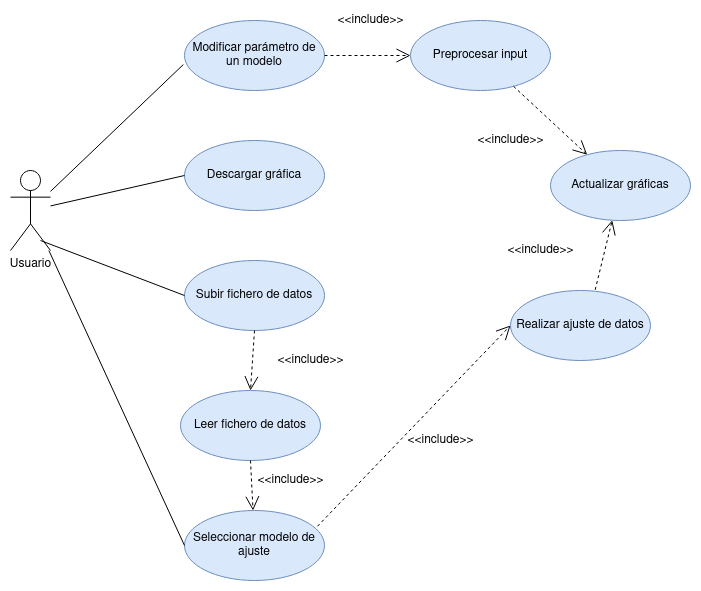
\includegraphics[scale=0.5]{casos_de_uso.drawio}
\end{center}
\end{figure}



\clearpage

\subsection{Plantillas de casos de uso}



\begin{table}[!h]
\begin{tabularx}{\textwidth}{|Y|Y|Y|Y|Y|Y|Y|Y|Y|}
\hline
\rowcolor{azulillo} \multicolumn{2}{|c|}{\textbf{Caso de uso}} & \multicolumn{5}{|c|}{Modificar parámetro de un modelo} & \multicolumn{2}{|c|}{CU-1} \\
\hline
\multicolumn{2}{|c|}{\cellcolor{azulillo} \textbf{Actores}}              & \multicolumn{7}{|c|}{Usuario}           \\
\hline
\multicolumn{2}{|c|}{\cellcolor{azulillo} \textbf{Tipo}}                 & \multicolumn{7}{|c|}{Esencial}             \\
\hline
\multicolumn{2}{|c|}{\cellcolor{azulillo} \textbf{Referencias}}          & \multicolumn{2}{|c|}{RF1}           & \multicolumn{5}{|c|}{CU-2, CU-5}\\
\hline
\multicolumn{2}{|c|}{\cellcolor{azulillo} \textbf{Precondición}}         & \multicolumn{7}{|c|}{Se debe estar trabajando con un modelo.}             \\
\hline
\multicolumn{2}{|c|}{\cellcolor{azulillo} \textbf{Postcondición}}        & \multicolumn{7}{|c|}{Se debe preprocesar la entrada.}              \\
\hline
\multicolumn{2}{|c|}{\cellcolor{azulillo} \textbf{Autor}}               &   Ana  & \multicolumn{2}{|c|}{\cellcolor{azulillo} \textbf{Fecha}} &  25/04/22   & \multicolumn{2}{|c|}{\cellcolor{azulillo} \textbf{Versión}} & 1.0  \\
\hline
\end{tabularx}
\end{table}

\begin{table}[!h]
\begin{tabularx}{\textwidth}{|Y|}
\hline
\cellcolor{azulillo} \textbf{Propósito} \\
\hline
Modificar uno de los parámetros disponibles del modelo para ver cómo afecta al  comportamiento del mismo.   \\
\hline
\end{tabularx}
\end{table}

\begin{table}[!h]
\begin{tabularx}{\textwidth}{|Y|}
\hline
\cellcolor{azulillo} \textbf{Resumen}  \\
\hline
Se modifica uno de los parámetros posibles del modelo, modificando así su comportamiento y visualizando la nueva gráfica resultante.   \\
\hline
\end{tabularx}
\end{table}

\begin{table}[!h]
\begin{tabularx}{\textwidth}{|c|Y|c|Y|}
\hline
\multicolumn{4}{|c|}{ \cellcolor{azulillo}Curso normal} \\
\hline
      1.        &  El usuario modifica un parámetro     &              &              \\
\hline
              &               &       2.       &      Incluir CU-2         \\
\hline
              &               &       3.       &      Incluir CU-5        \\

\hline
\end{tabularx}
\end{table}

\begin{table}[!h]
\begin{tabularx}{\textwidth}{|c|Y|}
\hline
\multicolumn{2}{|c|}{\cellcolor{azulillo} \textbf{Cursos alternos}} \\
\hline
       2a.       &      El formato no es correcto, se asigna un valor por defecto        \\
\hline
       3a.       &      Incluir CU-5        \\
\hline
\end{tabularx}
\end{table}

\begin{table}[!h]
\begin{tabularx}{\textwidth}{|Y|Y|Y|Y|}
\hline
\multicolumn{4}{|c|}{\cellcolor{azulillo} \textbf{Otros datos}} \\
\hline
 \cellcolor{azulillo} \textbf{Frecuencia esperada}             &     Alta          &    \cellcolor{azulillo} \textbf{Rendimiento}          &      Alto        \\
\hline
 \cellcolor{azulillo} \textbf{Importancia}             &      Vital         &     \cellcolor{azulillo} \textbf{Urgencia}         &      Alta        \\
\hline
 \cellcolor{azulillo} \textbf{Estado}             &      Finalizado         &    \cellcolor{azulillo} \textbf{Estabilidad}          &     Alta         \\
\hline
 \cellcolor{azulillo} \textbf{Comentarios}        &  \multicolumn{3}{|c|}{-} \\
\hline
\end{tabularx}
\end{table}





\clearpage

\begin{table}[!h]
\begin{tabularx}{\textwidth}{|Y|Y|Y|Y|Y|Y|Y|Y|Y|}
\hline
\rowcolor{azulillo} \multicolumn{2}{|c|}{\textbf{Caso de uso}} & \multicolumn{5}{|c|}{Preprocesar entrada} & \multicolumn{2}{|c|}{CU-2} \\
\hline
\multicolumn{2}{|c|}{\cellcolor{azulillo} \textbf{Actores} }             & \multicolumn{7}{|c|}{(Sistema)}           \\
\hline
\multicolumn{2}{|c|}{\cellcolor{azulillo} \textbf{Tipo}  }               & \multicolumn{7}{|c|}{Esencial}             \\
\hline
\multicolumn{2}{|c|}{\cellcolor{azulillo} \textbf{Referencias}  }        & \multicolumn{2}{|c|}{RF-1}           & \multicolumn{5}{|c|}{CU-1}\\
\hline
\multicolumn{2}{|c|}{\cellcolor{azulillo} \textbf{Precondición} }        & \multicolumn{7}{|c|}{Se debe haber modificado un parámetro del modelo.}             \\
\hline
\multicolumn{2}{|c|}{\cellcolor{azulillo} \textbf{Postcondición} }       & \multicolumn{7}{|c|}{Se debe actualizar la gráfica. }              \\
\hline
\multicolumn{2}{|c|}{\cellcolor{azulillo} \textbf{Autor}   }             &   Ana   & \multicolumn{2}{|c|}{\cellcolor{azulillo} \textbf{Fecha}} &  25/04/22   & \multicolumn{2}{|c|}{\cellcolor{azulillo} \textbf{Versión}} & 1.0  \\
\hline
\end{tabularx}
\end{table}

\begin{table}[!h]
\begin{tabularx}{\textwidth}{|Y|}
\hline
\cellcolor{azulillo} \textbf{Propósito} \\
\hline
Asegurar el correcto formato y validez del valor introducido. \\
\hline
\end{tabularx}
\end{table}

\begin{table}[!h]
\begin{tabularx}{\textwidth}{|Y|}
\hline
\cellcolor{azulillo} \textbf{Resumen}  \\
\hline
 Se comprueba la validez y formato del valor introducido para asegurar el correcto funcionamiento del modelo.  \\
\hline
\end{tabularx}
\end{table}

\begin{table}[!h]
\begin{tabularx}{\textwidth}{|c|Y|c|Y|}
\hline
\multicolumn{4}{|c|}{\cellcolor{azulillo} \textbf{Curso normal}} \\
\hline
              &               &      1.        &    Se comprueba el tipo de valor (float o entero).         \\
\hline
              &               &      2.        &    Se  comprueba el rango de validez de los valors de cada parámetro.         \\
\hline
              &               &      3.        &    Se comprueba que la población sea constante.          \\
\hline
\end{tabularx}
\end{table}

\begin{table}[!h]
\begin{tabularx}{\textwidth}{|c|Y|}
\hline
\multicolumn{2}{|c|}{\cellcolor{azulillo} \textbf{Cursos alternos}} \\
\hline
        1a       &     Si el valor no es de un tipo válido se sustituye por $0$. \\
\hline
        2b.      &     Si el valor no está en el rango se sustituye por $0$.         \\
\hline

\end{tabularx}
\end{table}

\begin{table}[!h]
\begin{tabularx}{\textwidth}{|Y|Y|Y|Y|}
\hline
\multicolumn{4}{|c|}{\cellcolor{azulillo} \textbf{Otros datos}} \\
\hline
 \cellcolor{azulillo} \textbf{Frecuencia esperada}             &      Alta         &    \cellcolor{azulillo} \textbf{Rendimiento}          &      Alto        \\
\hline
 \cellcolor{azulillo} \textbf{Importancia}             &      Vital         &     \cellcolor{azulillo} \textbf{Urgencia}         &      Alta        \\
\hline
 \cellcolor{azulillo} \textbf{Estado}             &       Finalizado        &    \cellcolor{azulillo} \textbf{Estabilidad}          &    Alta          \\
\hline
 \cellcolor{azulillo} \textbf{Comentarios}        &  \multicolumn{3}{|c|}{-} \\
\hline
\end{tabularx}
\end{table}






\clearpage

\begin{table}[!h]
\begin{tabularx}{\textwidth}{|Y|Y|Y|Y|Y|Y|Y|Y|Y|}
\hline
\rowcolor{azulillo} \multicolumn{2}{|c|}{\textbf{Caso de uso}} & \multicolumn{5}{|c|}{Subir fichero de datos} & \multicolumn{2}{|c|}{CU-3} \\
\hline
\multicolumn{2}{|c|}{\cellcolor{azulillo} \textbf{Actores}}              & \multicolumn{7}{|c|}{Usuario}           \\
\hline
\multicolumn{2}{|c|}{\cellcolor{azulillo} \textbf{Tipo} }                & \multicolumn{7}{|c|}{Esencial}             \\
\hline
\multicolumn{2}{|c|}{\cellcolor{azulillo} \textbf{Referencias}}          & \multicolumn{2}{|c|}{RF4}           & \multicolumn{5}{|c|}{CU-4, CU-5, CU-6, CU-7}\\
\hline
\multicolumn{2}{|c|}{\cellcolor{azulillo} \textbf{Precondición}}         & \multicolumn{7}{|c|}{-}             \\
\hline
\multicolumn{2}{|c|}{\cellcolor{azulillo} \textbf{Postcondición}}        & \multicolumn{7}{|c|}{-}              \\
\hline
\multicolumn{2}{|c|}{\cellcolor{azulillo} \textbf{Autor}  }              &   Ana  & \multicolumn{2}{|c|}{\cellcolor{azulillo} \textbf{Fecha}} &  25/04/22   & \multicolumn{2}{|c|}{\cellcolor{azulillo} \textbf{Versión}} & 1.0  \\
\hline
\end{tabularx}
\end{table}

\begin{table}[!h]
\begin{tabularx}{\textwidth}{|Y|}
\hline
\cellcolor{azulillo} \textbf{Propósito} \\
\hline
El usuario debe poder subir un fichero de datos para trabajar sobre él.  \\
\hline
\end{tabularx}
\end{table}

\begin{table}[!h]
\begin{tabularx}{\textwidth}{|Y|}
\hline
\cellcolor{azulillo} \textbf{Resumen}  \\
\hline
El usuario sube un fichero de datos.    \\
\hline
\end{tabularx}
\end{table}

\begin{table}[!h]
\begin{tabularx}{\textwidth}{|c|Y|c|Y|}
\hline
\multicolumn{4}{|c|}{\cellcolor{azulillo} \textbf{Curso normal}} \\
\hline
      1.        &      El usuario selecciona un fichero de datos.         &              &              \\
\hline
              &               &      2.        &    El sistema sube el fichero de datos seleccionado.          \\
\hline
\end{tabularx}
\end{table}

\begin{table}[!h]
\begin{tabularx}{\textwidth}{|c|Y|}
\hline
\multicolumn{2}{|c|}{\cellcolor{azulillo} \textbf{Cursos alternos}} \\
\hline
      2a.        &    El fichero no tiene formato correcto, por lo que no se deja seleccionarlo.          \\
\hline
\end{tabularx}
\end{table}

\begin{table}[!h]
\begin{tabularx}{\textwidth}{|Y|Y|Y|Y|}
\hline
\multicolumn{4}{|c|}{\cellcolor{azulillo} \textbf{Otros datos}} \\
\hline
 \cellcolor{azulillo} \textbf{Frecuencia esperada}             &     Alta          &    \cellcolor{azulillo} \textbf{Rendimiento}          &      Alto        \\
\hline
 \cellcolor{azulillo} \textbf{Importancia}             &      Vital         &     \cellcolor{azulillo} \textbf{Urgencia}         &      Alta        \\
\hline
 \cellcolor{azulillo} \textbf{Estado}             &      Finalizado         &    \cellcolor{azulillo} \textbf{Estabilidad}          &     Alta         \\
\hline
 \cellcolor{azulillo} \textbf{Comentarios}        &  \multicolumn{3}{|c|}{-} \\
\hline
\end{tabularx}
\end{table}




\clearpage

\begin{table}[!h]
\begin{tabularx}{\textwidth}{|Y|Y|Y|Y|Y|Y|Y|Y|Y|}
\hline
\rowcolor{azulillo} \multicolumn{2}{|c|}{\textbf{Caso de uso}} & \multicolumn{5}{|c|}{Leer fichero de datos} & \multicolumn{2}{|c|}{CU-4} \\
\hline
\multicolumn{2}{|c|}{\cellcolor{azulillo} \textbf{Actores}}              & \multicolumn{7}{|c|}{(Sistema)}           \\
\hline
\multicolumn{2}{|c|}{\cellcolor{azulillo} \textbf{Tipo}}                 & \multicolumn{7}{|c|}{Esencial}             \\
\hline
\multicolumn{2}{|c|}{\cellcolor{azulillo} \textbf{Referencias}}          & \multicolumn{2}{|c|}{RF4}           & \multicolumn{5}{|c|}{CU-3, CU-7}\\
\hline
\multicolumn{2}{|c|}{\cellcolor{azulillo} \textbf{Precondición}}         & \multicolumn{7}{|c|}{Se debe haber subido el fichero a leer.}             \\
\hline
\multicolumn{2}{|c|}{\cellcolor{azulillo} \textbf{Postcondición}}        & \multicolumn{7}{|c|}{Se debe actualizar la gráfica.}              \\
\hline
\multicolumn{2}{|c|}{\cellcolor{azulillo} \textbf{Autor} }               &   Ana   & \multicolumn{2}{|c|}{\cellcolor{azulillo} \textbf{Fecha}} &  25/04/22   & \multicolumn{2}{|c|}{\cellcolor{azulillo} \textbf{Versión}} & 1.0  \\
\hline
\end{tabularx}
\end{table}

\begin{table}[!h]
\begin{tabularx}{\textwidth}{|Y|}
\hline
\cellcolor{azulillo} \textbf{Propósito} \\
\hline
 Leer el fichero para poder trabajar con los datos que contiene.                  \\
\hline
\end{tabularx}
\end{table}

\begin{table}[!h]
\begin{tabularx}{\textwidth}{|Y|}
\hline
\cellcolor{azulillo} \textbf{Resumen}  \\
\hline
 Se lee el fichero de datos cargando estos en memoria.                  \\
\hline
\end{tabularx}
\end{table}

\begin{table}[!h]
\begin{tabularx}{\textwidth}{|c|Y|c|Y|}
\hline
\multicolumn{4}{|c|}{\cellcolor{azulillo} \textbf{Curso normal}} \\
\hline
              &               &      1.        &     Se abre el fichero         \\
\hline
              &               &      2.        &     Se lee el fichero         \\
\hline
\end{tabularx}
\end{table}

\begin{table}[!h]
\begin{tabularx}{\textwidth}{|c|Y|}
\hline
\multicolumn{2}{|c|}{\cellcolor{azulillo} \textbf{Cursos alternos}} \\
\hline
    2a.          &      Si el formato del fichero no es el esperado, se muestra un error.        \\
\hline
\end{tabularx}
\end{table}

\begin{table}[!h]
\begin{tabularx}{\textwidth}{|Y|Y|Y|Y|}
\hline
\multicolumn{4}{|c|}{\cellcolor{azulillo} \textbf{Otros datos}} \\
\hline
 \cellcolor{azulillo} \textbf{Frecuencia esperada}             &      Alta         &    \cellcolor{azulillo} \textbf{Rendimiento}          &      Alto        \\
\hline
 \cellcolor{azulillo} \textbf{Importancia}             &       Vital        &     \cellcolor{azulillo} \textbf{Urgencia}         &      Alta        \\
\hline
 \cellcolor{azulillo} \textbf{Estado}             &       Finalizado        &    \cellcolor{azulillo} \textbf{Estabilidad}          &      Alta        \\
\hline
 \cellcolor{azulillo} \textbf{Comentarios}        &  \multicolumn{3}{|c|}{-} \\
\hline
\end{tabularx}
\end{table}





\clearpage

\begin{table}[!h]
\begin{tabularx}{\textwidth}{|Y|Y|Y|Y|Y|Y|Y|Y|Y|}
\hline
\rowcolor{azulillo} \multicolumn{2}{|c|}{\textbf{Caso de uso}} & \multicolumn{5}{|c|}{Actualizar gráficas} & \multicolumn{2}{|c|}{CU-5} \\
\hline
\multicolumn{2}{|c|}{\cellcolor{azulillo} \textbf{Actores} }             & \multicolumn{7}{|c|}{(Sistema)}           \\
\hline
\multicolumn{2}{|c|}{\cellcolor{azulillo} \textbf{Tipo}  }               & \multicolumn{7}{|c|}{Esencial}             \\
\hline
\multicolumn{2}{|c|}{\cellcolor{azulillo} \textbf{Referencias} }         & \multicolumn{2}{|c|}{RF1, RF2, RF5}           & \multicolumn{5}{|c|}{CU-1, CU-6}\\
\hline
\multicolumn{2}{|c|}{\cellcolor{azulillo} \textbf{Precondición}}         & \multicolumn{7}{|c|}{Se ha modificado un parámetro o ajuste seleccionado.}             \\
\hline
\multicolumn{2}{|c|}{\cellcolor{azulillo} \textbf{Postcondición}  }      & \multicolumn{7}{|c|}{La gráfica se ha actualizado.}              \\
\hline
\multicolumn{2}{|c|}{\cellcolor{azulillo} \textbf{Autor}   }             &   Ana   & \multicolumn{2}{|c|}{\cellcolor{azulillo} \textbf{Fecha}} &  25/04/22   & \multicolumn{2}{|c|}{\cellcolor{azulillo} \textbf{Versión}} & 1.0  \\
\hline
\end{tabularx}
\end{table}

\begin{table}[!h]
\begin{tabularx}{\textwidth}{|Y|}
\hline
\cellcolor{azulillo} \textbf{Propósito} \\
\hline
Actualizar la gráfica para tener la visualización de los datos de acuerdo a las opciones indicadas.   \\
\hline
\end{tabularx}
\end{table}

\begin{table}[!h]
\begin{tabularx}{\textwidth}{|Y|}
\hline
\cellcolor{azulillo} \textbf{Resumen}  \\
\hline
Actualizar la gráfica cuando el usuario realiza una modificación de parámetros o del modelo con el que realizar el ajuste.  \\
\hline
\end{tabularx}
\end{table}

\begin{table}[!h]
\begin{tabularx}{\textwidth}{|c|Y|c|Y|}
\hline
\multicolumn{4}{|c|}{\cellcolor{azulillo} \textbf{Curso normal}} \\
\hline
              &               &      1.        &     Incluir CU-4         \\
\hline
              &               &      2.        &     Representar los datos con el nuevo parámetro.         \\
\hline
\end{tabularx}
\end{table}

\begin{table}[!h]
\begin{tabularx}{\textwidth}{|c|Y|}
\hline
\multicolumn{2}{|c|}{\cellcolor{azulillo} \textbf{Cursos alternos}} \\
\hline
      2a.        &     Si se ha cambiado el modelo con el que realizar el ajuste, incluir CU-7.         \\
\hline
      3a.        &     Representar los datos con el nuevo ajuste.         \\
\hline
\end{tabularx}
\end{table}

\begin{table}[!h]
\begin{tabularx}{\textwidth}{|Y|Y|Y|Y|}
\hline
\multicolumn{4}{|c|}{\cellcolor{azulillo} \textbf{Otros datos}} \\
\hline
 \cellcolor{azulillo} \textbf{Frecuencia esperada}             &     Alta         &    \cellcolor{azulillo} \textbf{Rendimiento}          &      Medio        \\
\hline
 \cellcolor{azulillo} \textbf{Importancia}             &      Vital         &     \cellcolor{azulillo} \textbf{Urgencia}         &     Alta         \\
\hline
 \cellcolor{azulillo} \textbf{Estado}             &       Finalizado        &    \cellcolor{azulillo} \textbf{Estabilidad}          &     Alta         \\
\hline
 \cellcolor{azulillo} \textbf{Comentarios}        &  \multicolumn{3}{|c|}{-} \\
\hline
\end{tabularx}
\end{table}




\clearpage

\begin{table}[!h]
\begin{tabularx}{\textwidth}{|Y|Y|Y|Y|Y|Y|Y|Y|Y|}
\hline
\rowcolor{azulillo} \multicolumn{2}{|c|}{\textbf{Caso de uso}} & \multicolumn{5}{|c|}{Seleccionar modelo de ajuste} & \multicolumn{2}{|c|}{CU-6} \\
\hline
\multicolumn{2}{|c|}{\cellcolor{azulillo} \textbf{Actores}}              & \multicolumn{7}{|c|}{Usuario}           \\
\hline
\multicolumn{2}{|c|}{\cellcolor{azulillo} \textbf{Tipo}}                 & \multicolumn{7}{|c|}{Esencial}             \\
\hline
\multicolumn{2}{|c|}{\cellcolor{azulillo} \textbf{Referencias}}          & \multicolumn{2}{|c|}{RF2}           & \multicolumn{5}{|c|}{CU-5, CU-7}\\
\hline
\multicolumn{2}{|c|}{\cellcolor{azulillo} \textbf{Precondición} }        & \multicolumn{7}{|c|}{Se debe tener leído un fichero de datos.}             \\
\hline
\multicolumn{2}{|c|}{\cellcolor{azulillo} \textbf{Postcondición}}        & \multicolumn{7}{|c|}{Se debe realizar el ajuste con el nuevo modelo elegido.}              \\
\hline
\multicolumn{2}{|c|}{\cellcolor{azulillo} \textbf{Autor}}                &   Ana   & \multicolumn{2}{|c|}{\cellcolor{azulillo} \textbf{Fecha}} &  25/04/22   & \multicolumn{2}{|c|}{\cellcolor{azulillo} \textbf{Versión}} & 1.0  \\
\hline
\end{tabularx}
\end{table}

\begin{table}[!h]
\begin{tabularx}{\textwidth}{|Y|}
\hline
\cellcolor{azulillo} \textbf{Propósito} \\
\hline
Poder elegir el modelo con el que realizar el ajuste de los datos.  \\
\hline
\end{tabularx}
\end{table}

\begin{table}[!h]
\begin{tabularx}{\textwidth}{|Y|}
\hline
\cellcolor{azulillo} \textbf{Resumen}  \\
\hline
Seleccionar el modelo a partir del cuál se va a realizar el ajuste.  \\
\hline
\end{tabularx}
\end{table}

\begin{table}[!h]
\begin{tabularx}{\textwidth}{|c|Y|c|Y|}
\hline
\multicolumn{4}{|c|}{\cellcolor{azulillo} \textbf{Curso normal}} \\
\hline
      1.        &     El usuario selecciona un modelo         &              &              \\
\hline
              &               &      2.        &      Incluir CU-7        \\
\hline
              &               &      3.        &      Incluir CU-5        \\
\hline
\end{tabularx}
\end{table}

\begin{table}[!h]
\begin{tabularx}{\textwidth}{|c|Y|}
\hline
\multicolumn{2}{|c|}{\cellcolor{azulillo} \textbf{Cursos alternos}} \\
\hline
              &       -       \\
\hline
\end{tabularx}
\end{table}

\begin{table}[!h]
\begin{tabularx}{\textwidth}{|Y|Y|Y|Y|}
\hline
\multicolumn{4}{|c|}{\cellcolor{azulillo} \textbf{Otros datos}} \\
\hline
 \cellcolor{azulillo} \textbf{Frecuencia esperada}             &       Alta        &    \cellcolor{azulillo} \textbf{Rendimiento}          &       Alto       \\
\hline
 \cellcolor{azulillo} \textbf{Importancia}             &      Alta         &     \cellcolor{azulillo} \textbf{Urgencia}         &       Alta       \\
\hline
 \cellcolor{azulillo} \textbf{Estado}             &      Finalizado         &    \cellcolor{azulillo} \textbf{Estabilidad}          &      Alta        \\
\hline
 \cellcolor{azulillo} \textbf{Comentarios}        &  \multicolumn{3}{|c|}{-} \\
\hline
\end{tabularx}
\end{table}





\clearpage

\begin{table}[!h]
\begin{tabularx}{\textwidth}{|Y|Y|Y|Y|Y|Y|Y|Y|Y|}
\hline
\rowcolor{azulillo} \multicolumn{2}{|c|}{\textbf{Caso de uso}} & \multicolumn{5}{|c|}{Realizar ajuste de datos} & \multicolumn{2}{|c|}{CU-7} \\
\hline
\multicolumn{2}{|c|}{\cellcolor{azulillo} \textbf{Actores} }             & \multicolumn{7}{|c|}{(Sistema)}           \\
\hline
\multicolumn{2}{|c|}{\cellcolor{azulillo} \textbf{Tipo} }                & \multicolumn{7}{|c|}{Esencial}             \\
\hline
\multicolumn{2}{|c|}{\cellcolor{azulillo} \textbf{Referencias} }         & \multicolumn{2}{|c|}{RF6, RF7}           & \multicolumn{5}{|c|}{CU-3, CU-4, CU-5, CU-6}\\
\hline
\multicolumn{2}{|c|}{\cellcolor{azulillo} \textbf{Precondición}}         & \multicolumn{7}{|c|}{Se debe haber leído un fichero y seleccionado un modelo.}             \\
\hline
\multicolumn{2}{|c|}{\cellcolor{azulillo} \textbf{Postcondición}}        & \multicolumn{7}{|c|}{Actualizar las gráficas}              \\
\hline
\multicolumn{2}{|c|}{\cellcolor{azulillo} \textbf{Autor} }               &   Ana   & \multicolumn{2}{|c|}{\cellcolor{azulillo} \textbf{Fecha}} &  25/04/22   & \multicolumn{2}{|c|}{\cellcolor{azulillo} \textbf{Versión}} & 1.0  \\
\hline
\end{tabularx}
\end{table}

\begin{table}[!h]
\begin{tabularx}{\textwidth}{|Y|}
\hline
\cellcolor{azulillo} \textbf{Propósito} \\
\hline
Obtener una estimación de los parámetros y los errores correspondientes de acuerdo al modelo seleccionado. \\
\hline
\end{tabularx}
\end{table}

\begin{table}[!h]
\begin{tabularx}{\textwidth}{|Y|}
\hline
\cellcolor{azulillo} \textbf{Resumen}  \\
\hline
Se realiza el ajuste de un modelo elegido a los datos leídos. \\
\hline
\end{tabularx}
\end{table}

\begin{table}[!h]
\begin{tabularx}{\textwidth}{|c|Y|c|Y|}
\hline
\multicolumn{4}{|c|}{\cellcolor{azulillo} \textbf{Curso normal}} \\
\hline
     1.         &     Incluir CU-6           &              &              \\
\hline
              &               &    2.          &     Estimar parámetros         \\
\hline
              &               &    3.          &     Calcular errores         \\
\hline
              &               &    4.          &     Incluir CU-5            \\
\hline
\end{tabularx}
\end{table}

\begin{table}[!h]
\begin{tabularx}{\textwidth}{|c|Y|}
\hline
\multicolumn{2}{|c|}{\cellcolor{azulillo} \textbf{Cursos alternos}} \\
\hline
     2a.         &    Si se debe elegir el mejor modelo, se calculan los parámetros para todos los modelos          \\
\hline
     3a.         &    Se calculan los errores para todos los modelos          \\
\hline
     4a.         &    Se elige el mejor modelo de acuerdo a un criterio sobre los errores          \\
\hline
\end{tabularx}
\end{table}

\begin{table}[!h]
\begin{tabularx}{\textwidth}{|Y|Y|Y|Y|}
\hline
\multicolumn{4}{|c|}{\cellcolor{azulillo} \textbf{Otros datos}} \\
\hline
 \cellcolor{azulillo} \textbf{Frecuencia esperada}             &      Alta         &    \cellcolor{azulillo} \textbf{Rendimiento}          &      Alto        \\
\hline
 \cellcolor{azulillo} \textbf{Importancia}             &      Vital         &     \cellcolor{azulillo} \textbf{Urgencia}         &      Alta        \\
\hline
 \cellcolor{azulillo} \textbf{Estado}             &       Finalizado        &    \cellcolor{azulillo} \textbf{Estabilidad}          &     Alta         \\
\hline
\cellcolor{azulillo} \textbf{Comentarios}        &  \multicolumn{3}{|c|}{-} \\
\hline
\end{tabularx}
\end{table}



\clearpage

\begin{table}[!h]
\begin{tabularx}{\textwidth}{|Y|Y|Y|Y|Y|Y|Y|Y|Y|}
\hline
\rowcolor{azulillo} \multicolumn{2}{|c|}{\textbf{Caso de uso}} & \multicolumn{5}{|c|}{Descargar gráfica} & \multicolumn{2}{|c|}{CU-8} \\
\hline
\multicolumn{2}{|c|}{\cellcolor{azulillo} \textbf{Actores} }             & \multicolumn{7}{|c|}{Usuario}           \\
\hline
\multicolumn{2}{|c|}{\cellcolor{azulillo} \textbf{Tipo}}                 & \multicolumn{7}{|c|}{Secundario}             \\
\hline
\multicolumn{2}{|c|}{\cellcolor{azulillo} \textbf{Referencias}}          & \multicolumn{2}{|c|}{RF3}           & \multicolumn{5}{|c|}{}\\
\hline
\multicolumn{2}{|c|}{\cellcolor{azulillo} \textbf{Precondición} }        & \multicolumn{7}{|c|}{-}             \\
\hline
\multicolumn{2}{|c|}{\cellcolor{azulillo} \textbf{Postcondición}}        & \multicolumn{7}{|c|}{-}              \\
\hline
\multicolumn{2}{|c|}{\cellcolor{azulillo} \textbf{Autor} }               &   Ana   & \multicolumn{2}{|c|}{\cellcolor{azulillo} \textbf{Fecha}} &  25/04/22   & \multicolumn{2}{|c|}{\cellcolor{azulillo} \textbf{Versión}} & 1.0  \\
\hline
\end{tabularx}
\end{table}

\begin{table}[!h]
\begin{tabularx}{\textwidth}{|Y|}
\hline
\cellcolor{azulillo} \textbf{Propósito} \\
\hline
Descargar una gráfica generada por la aplicación web. \\
\hline
\end{tabularx}
\end{table}

\begin{table}[!h]
\begin{tabularx}{\textwidth}{|Y|}
\hline
\cellcolor{azulillo} \textbf{Resumen}  \\
\hline
Se descarga la imagen de una gráfica generada. \\
\hline
\end{tabularx}
\end{table}

\begin{table}[!h]
\begin{tabularx}{\textwidth}{|c|Y|c|Y|}
\hline
\multicolumn{4}{|c|}{\cellcolor{azulillo} \textbf{Curso normal}} \\
\hline
     1.         &     Pulsa en descargar imagen           &              &              \\
\hline
              &               &    2.          &     Muestra el selector de archivos         \\
\hline
     3.         &     Selecciona dónde guardar el archivo          &              &             \\
\hline
               &                                            &    4.   & Se genera y descarga la imagen \\
\hline
\end{tabularx}
\end{table}

\begin{table}[!h]
\begin{tabularx}{\textwidth}{|c|Y|}
\hline
\multicolumn{2}{|c|}{\cellcolor{azulillo} \textbf{Cursos alternos}} \\
\hline
     3a.         &    El usuario cancela la descarga.    \\
\hline
\end{tabularx}
\end{table}

\begin{table}[!h]
\begin{tabularx}{\textwidth}{|Y|Y|Y|Y|}
\hline
\multicolumn{4}{|c|}{\cellcolor{azulillo} \textbf{Otros datos}} \\
\hline
 \cellcolor{azulillo} \textbf{Frecuencia esperada}             &      Baja         &    \cellcolor{azulillo} \textbf{Rendimiento}          &      Alto        \\
\hline
 \cellcolor{azulillo} \textbf{Importancia}             &      Baja         &     \cellcolor{azulillo} \textbf{Urgencia}         &      Baja        \\
\hline
 \cellcolor{azulillo} \textbf{Estado}             &       Finalizado        &    \cellcolor{azulillo} \textbf{Estabilidad}          &     Alta         \\
\hline
\cellcolor{azulillo} \textbf{Comentarios}        &  \multicolumn{3}{|c|}{-} \\
\hline
\end{tabularx}
\end{table}

\clearpage

\section{Diagramas de actividad}

Para facilitar la comprensión del funcionamiento de las distintas funcionalidades del sistema, se han realizado diagramas de actividad de sus funcionalidades más importantes, siendo estas la posible modificación de los parámetros de los modelos interactivos y el ajuste de datos subidos mediante un fichero de datos.

El diagrama de actividad correspondiente a la modificación de parámetros en los modelos se muestra en \eqref{diag: actividad_modificacion} y el del ajuste de parámetros se puede ver en \eqref{diag: actividad_ajuste}.

\begin{figure}[!h]
\begin{center}
\caption{Diagrama de actividad de la modificación de parámetros en un modelo.}
\label{diag: actividad_modificacion}
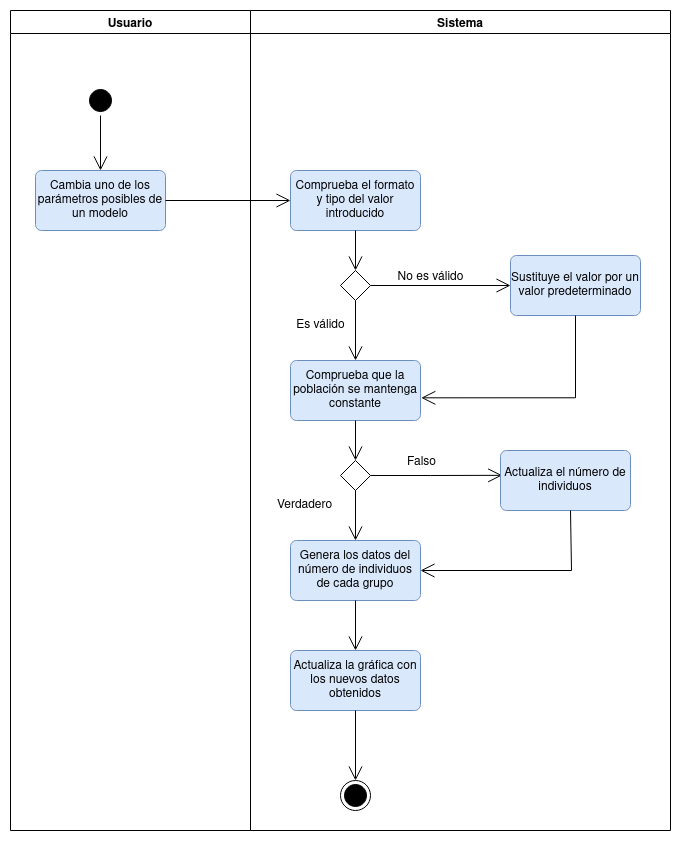
\includegraphics[scale=0.5]{diagrama_actividad-Modificar_parametro.drawio}
\end{center}
\end{figure}

\begin{figure}[!h]
\begin{center}
\caption{Diagrama de actividad del ajuste de datos.}
\label{diag: actividad_ajuste}
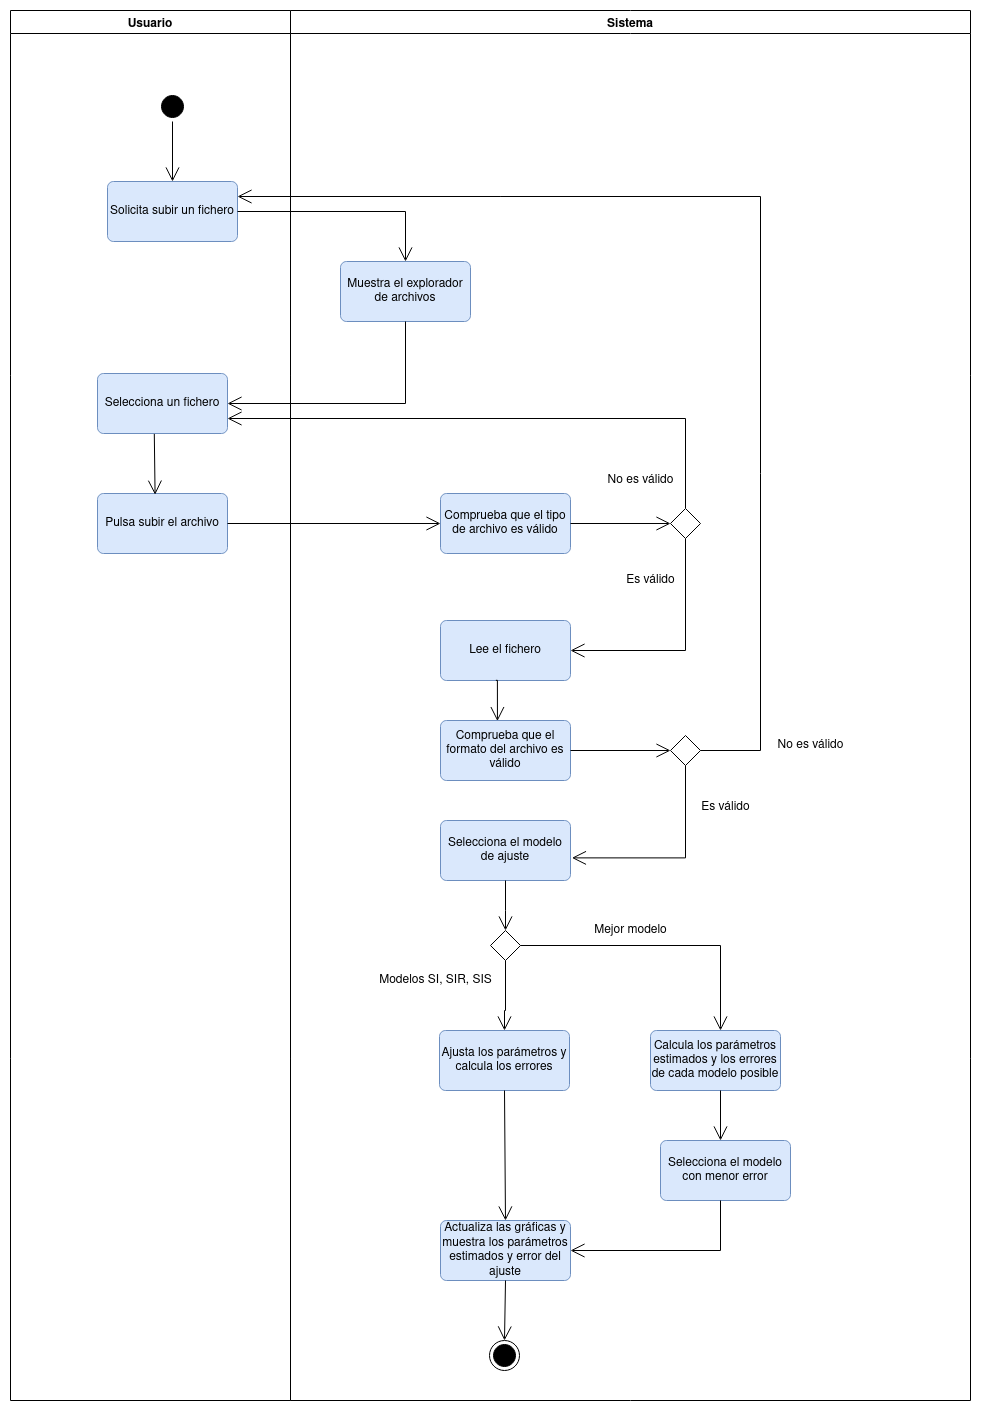
\includegraphics[scale=0.4]{diagrama_actividad-Ajuste_parametros.drawio}
\end{center}
\end{figure}


\section{Pruebas}

A medida que se desarrollaba el proyecto, se han llevado a cabo diversas pruebas de las distintas funcionalidades que se han desarrollado incrementalmente, con el fin de garantizar en todo momento que se disponía de un producto mínimamente viable.

Se han llevado a cabo dos tipos de pruebas:

\begin{itemize}
\item \textbf{Pruebas unitarias:} Tienen como objetivo asegurar el correcto funcionamiento de las funciones creadas de forma independiente de las demás. 
\item \textbf{Pruebas de usuario:} Tratan de simular la interacción entre un usuario y la interfaz del proyecto.
\end{itemize}

\subsection{Pruebas unitarias}

\begin{itemize}
\item \textbf{Preprocesamiento de valores de parámetros.} Se ha probado a introducir diversos valores para los parámetros modificables en los modelos interactivos, con el fin de asegurarnos de que se preprocesan adecuadamente. El comportamiento esperado es sustituir el valor introducido por $0$ en caso de que este sea un carácter o un valor negativo.
\item \textbf{Correcta generación de datos para diversos modelos.} Se han representado gráficamente los datos generados por las funciones de los modelos y contrastando el comportamiento de los datos obtenidos con el descrito en la teoría, asegurando así la correcta generación de los datos de acuerdo a los diversos modelos.
\item \textbf{Subida de ficheros.} Se ha probado a subir ficheros con extensiones permitidas (csv y txt) y comprobado que se han copiado al directorio pertinente para disponer de los ficheros cuando se requiera, así como a subir ficheros con extensiones no permitidas, verificando que se muestra el error pertinente al no permitirse.
\end{itemize}

\subsection{Pruebas de usuario}

\begin{itemize}
\item \textbf{Prueba de población constante.} Si el usuario introduce valores para las condiciones iniciales ($S_0, I_0$ y $R_0$ si es pertinente) tal que su suma no sea $N$ se actualiza el valor de la población de forma que $S_0+I_0+R_0=N$.
\item \textbf{Formato de los valores para parámetros.} Si el usuario introduce un valor de un parámetro con formato incorrecto se sustituye por $0$.
\item \textbf{Condiciones iniciales son números enteros.} Si el usuario introduce un valor no entero positivo se toma como valor real la parte entera del valor introducido por el usuario.
\item \textbf{Subida de fichero inexistente.} Si se trata de subir un fichero al que no se puede acceder o no selecciona ningún fichero antes de pulsar en subir fichero se muestra el error pertinente.
\item \textbf{Interacción con las gráficas.} Los usuarios pueden hacer zoom, desplazarse y obtener el valor numérico de las representaciones gráficas en cada momento en tiempo real, así como descargar las gráficas generadas.
\end{itemize}

%\clearpage

\section{Diseño de la interfaz de usuario}

Para finalizar el diseño del proyecto, hemos realizado unos prototipos del aspecto aproximado que tendrá la interfaz de la página web en algunas de sus páginas. Se ha tratado de conseguir una interfaz sencilla e intuitiva, que permita al usuario una navegación clara y eficaz por la página web, resultando así cómoda desde el primer momento.

Los prototipos de la interfaz se muestran en las figuras \eqref{wire: home}, \eqref{wire: home_desplegable}, \eqref{wire: modelo_interactivo}, \eqref{wire: ajuste} y \eqref{wire: ayuda}.

\begin{figure}
\begin{center}
\caption{Prototipo de la página home.}
\label{wire: home}
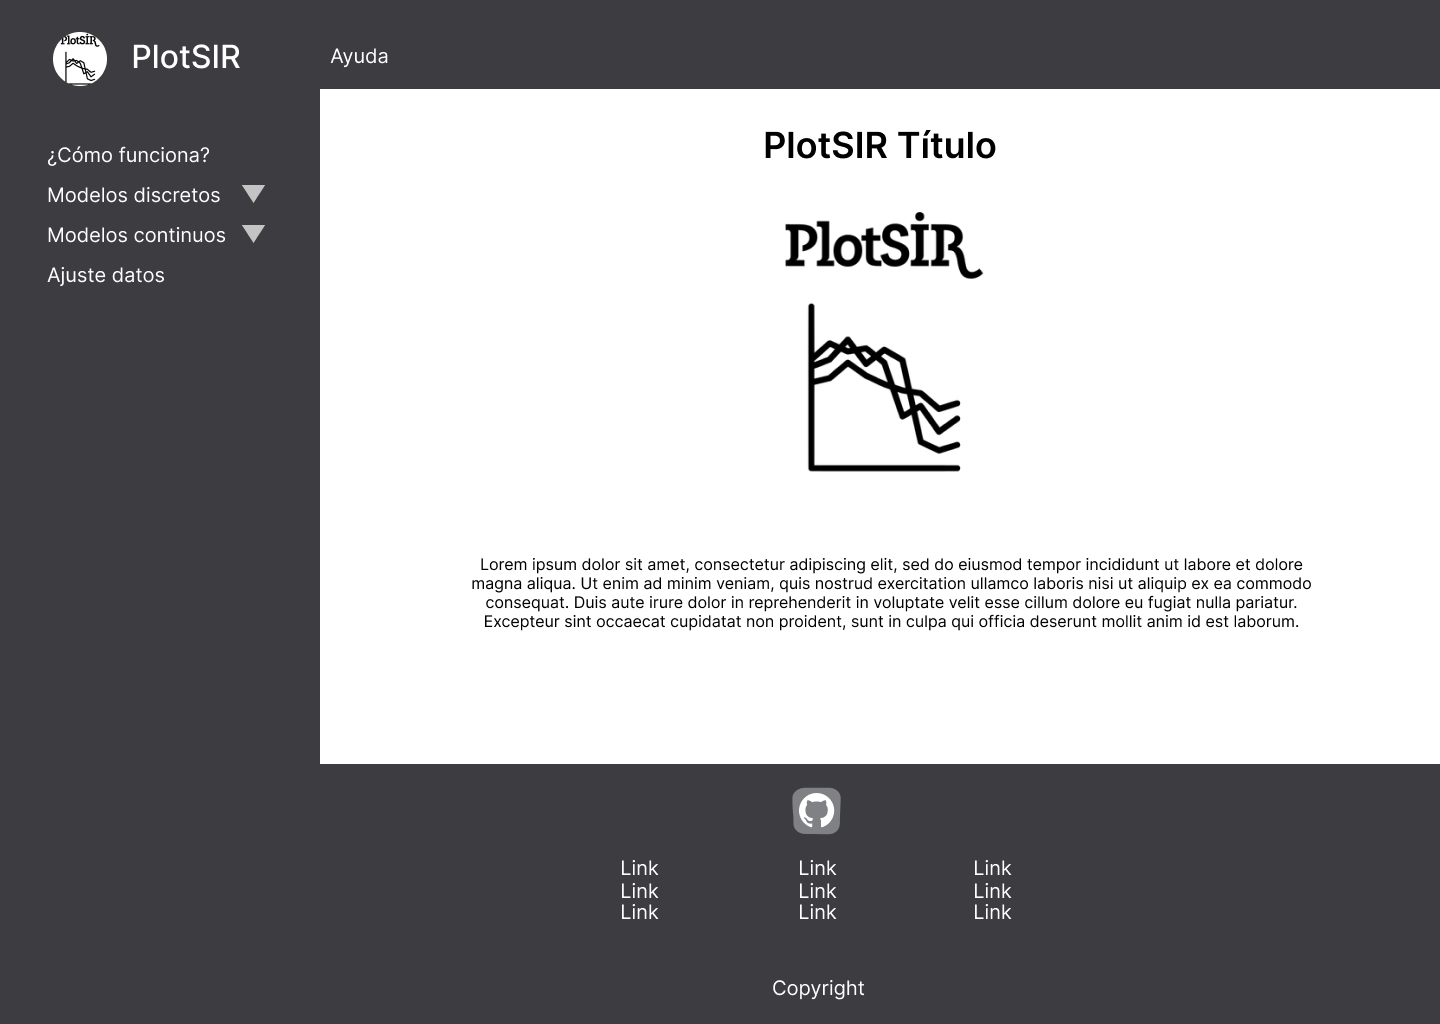
\includegraphics[scale=0.25]{Home}
\end{center}
\end{figure}

\begin{figure}
\begin{center}
\caption{Prototipo de la página home, con desplegable mostrándose.}
\label{wire: home_desplegable}
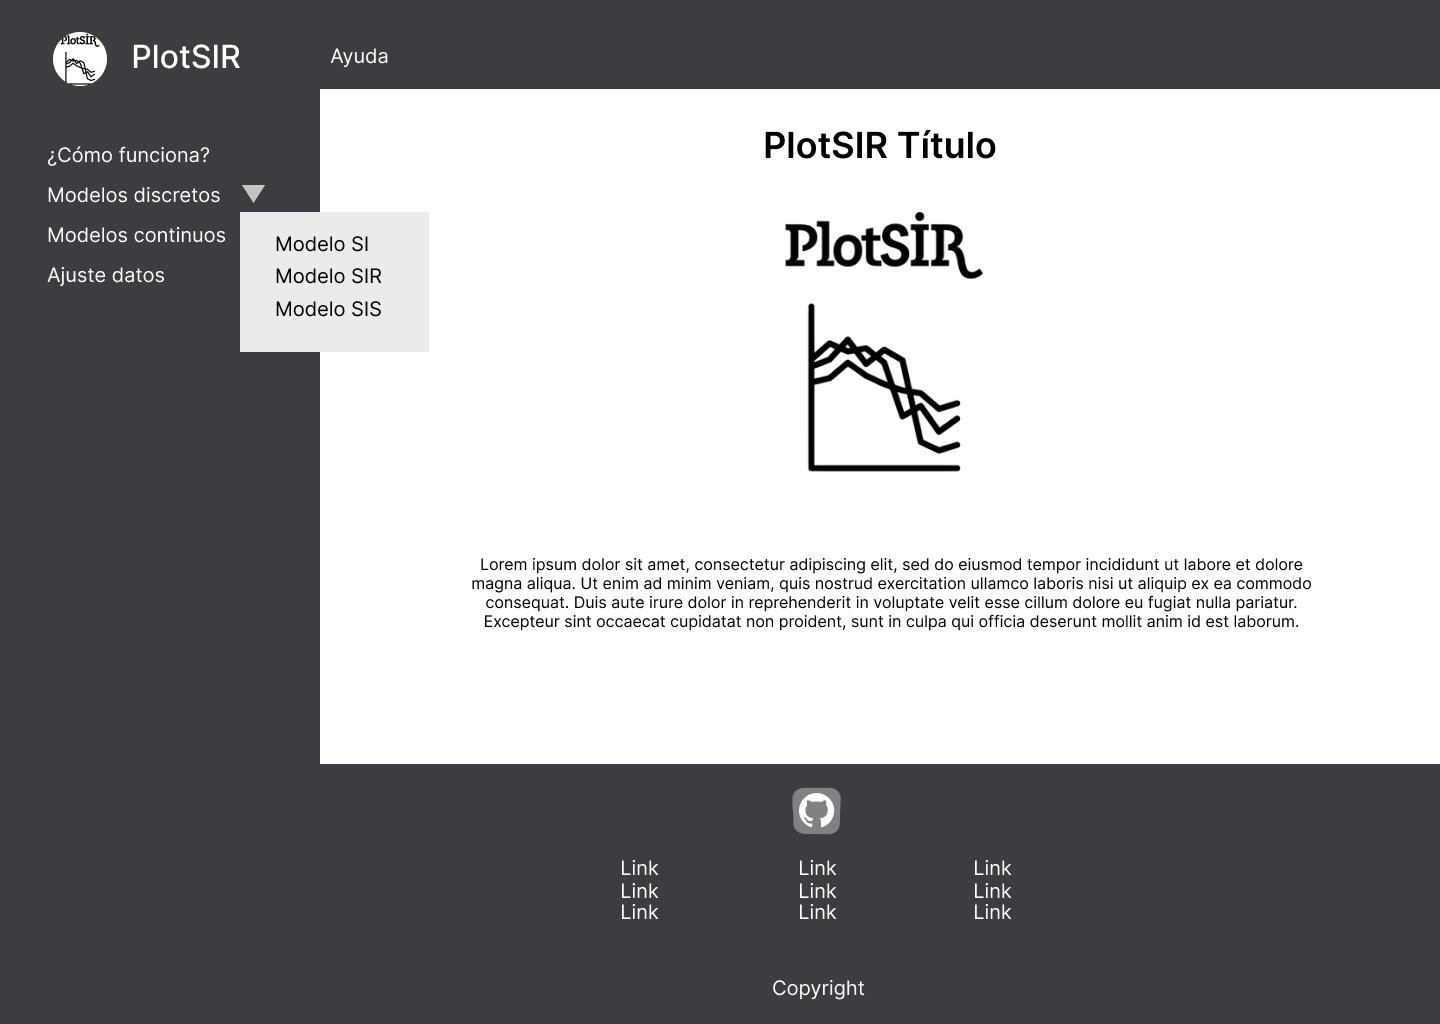
\includegraphics[scale=0.25]{Home_desplegable}
\end{center}
\end{figure}

\begin{figure}
\begin{center}
\caption{Prototipo de la página de un modelo interactivo.}
\label{wire: modelo_interactivo}
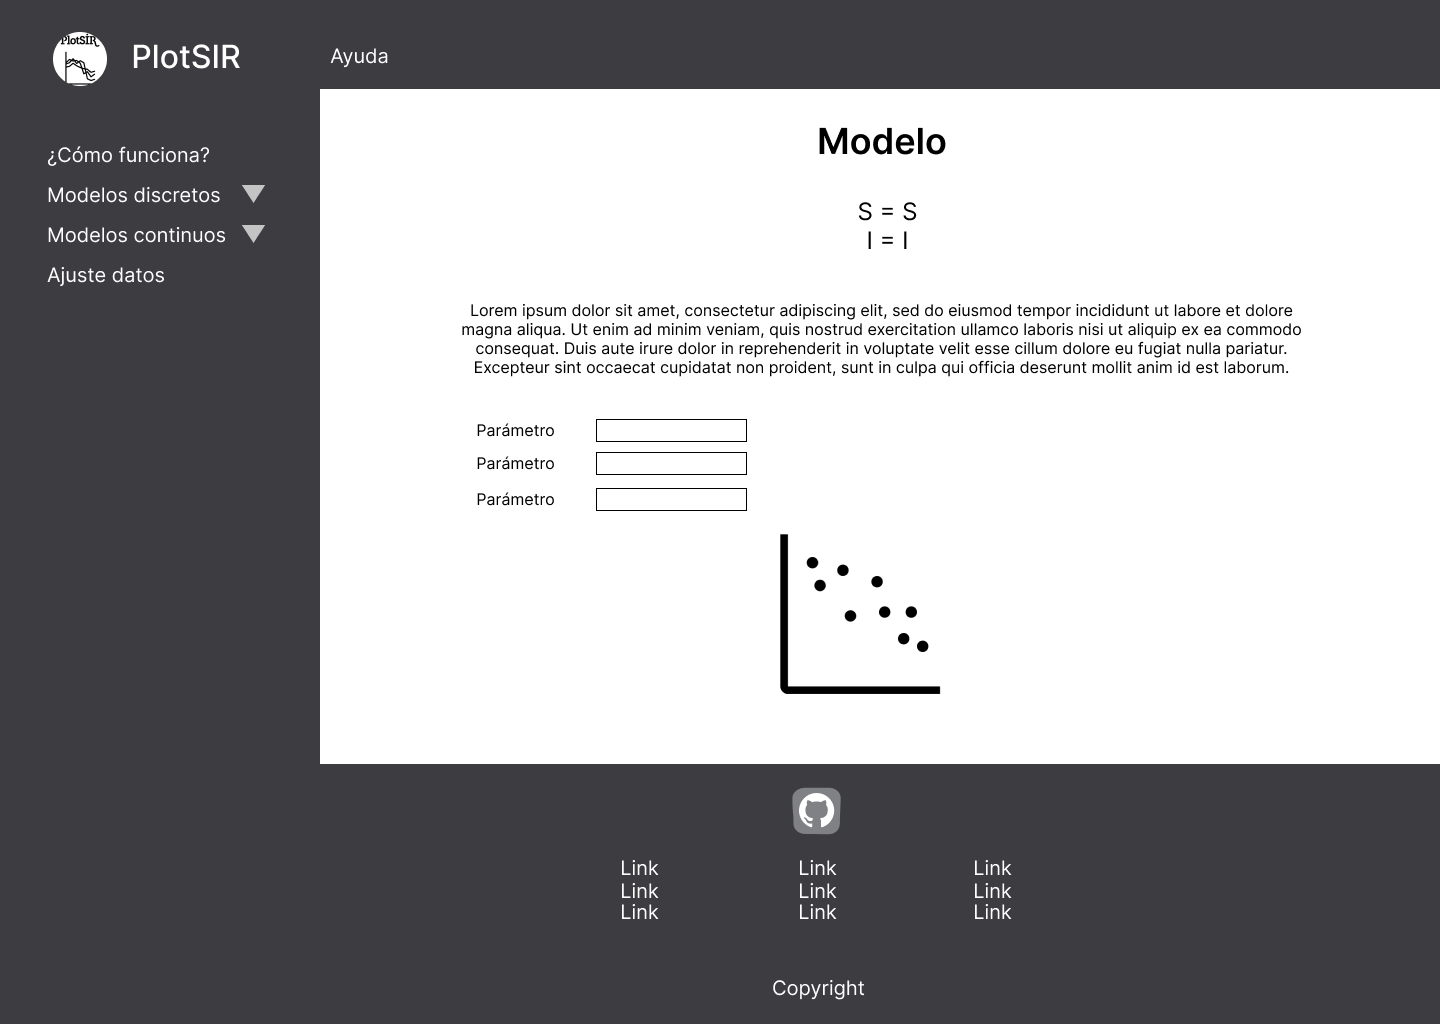
\includegraphics[scale=0.25]{Modelo_interactivo}
\end{center}
\end{figure}

\begin{figure}
\begin{center}
\caption{Prototipo de la página de ajuste de datos subidos desde un fichero.}
\label{wire: ajuste}
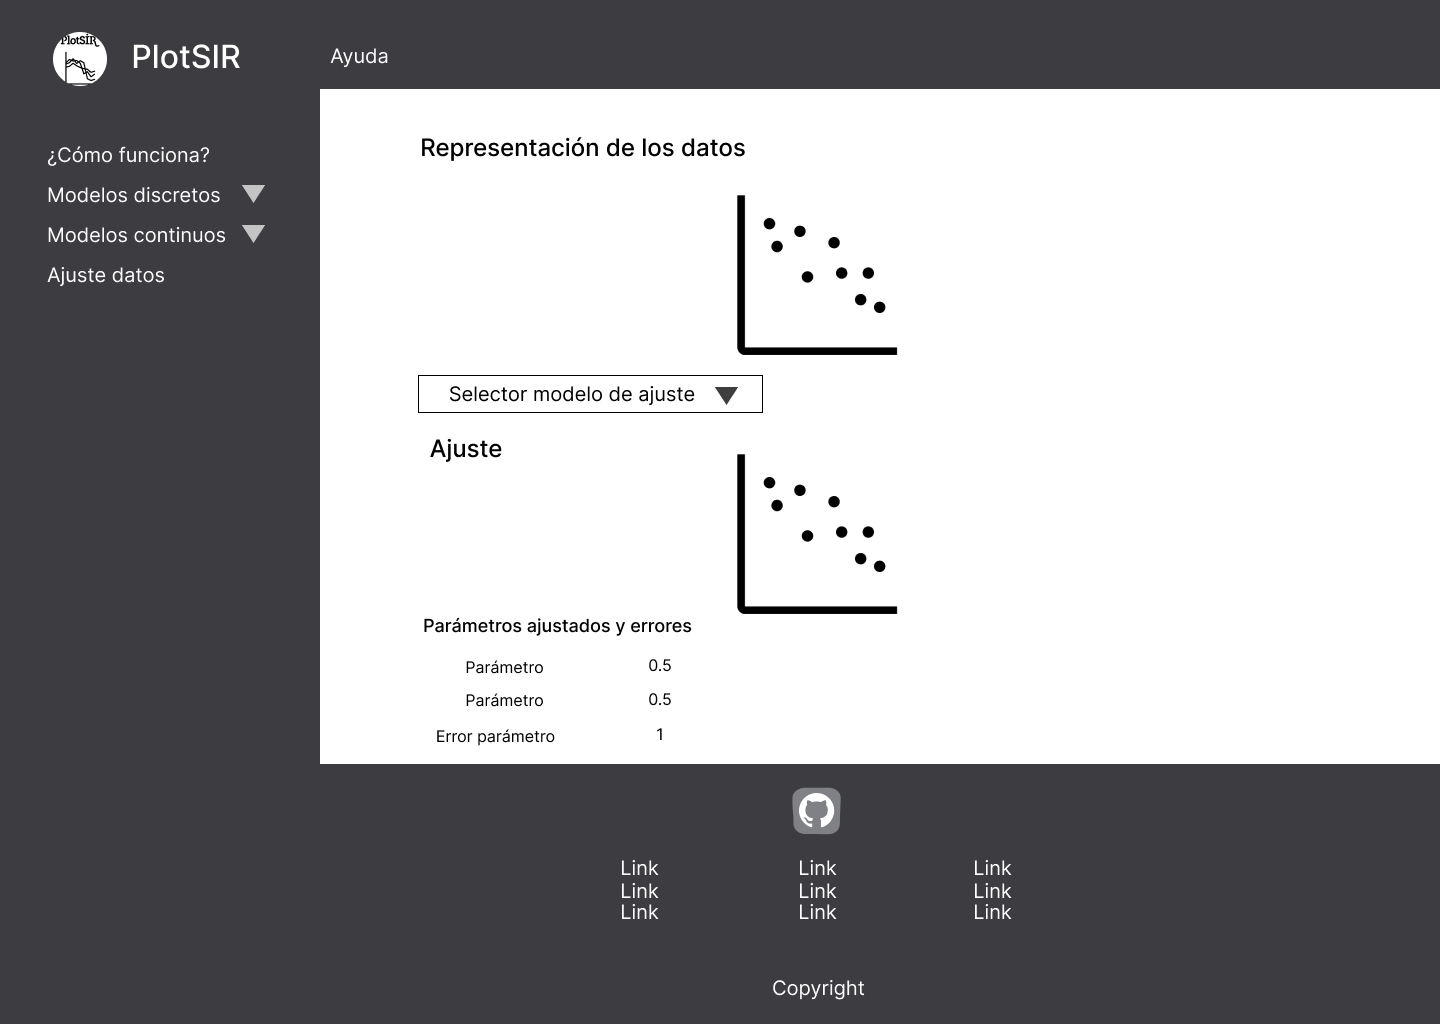
\includegraphics[scale=0.25]{Ajuste_datos}
\end{center}
\end{figure}

\begin{figure}
\begin{center}
\caption{Prototipo de la página de ayuda.}
\label{wire: ayuda}
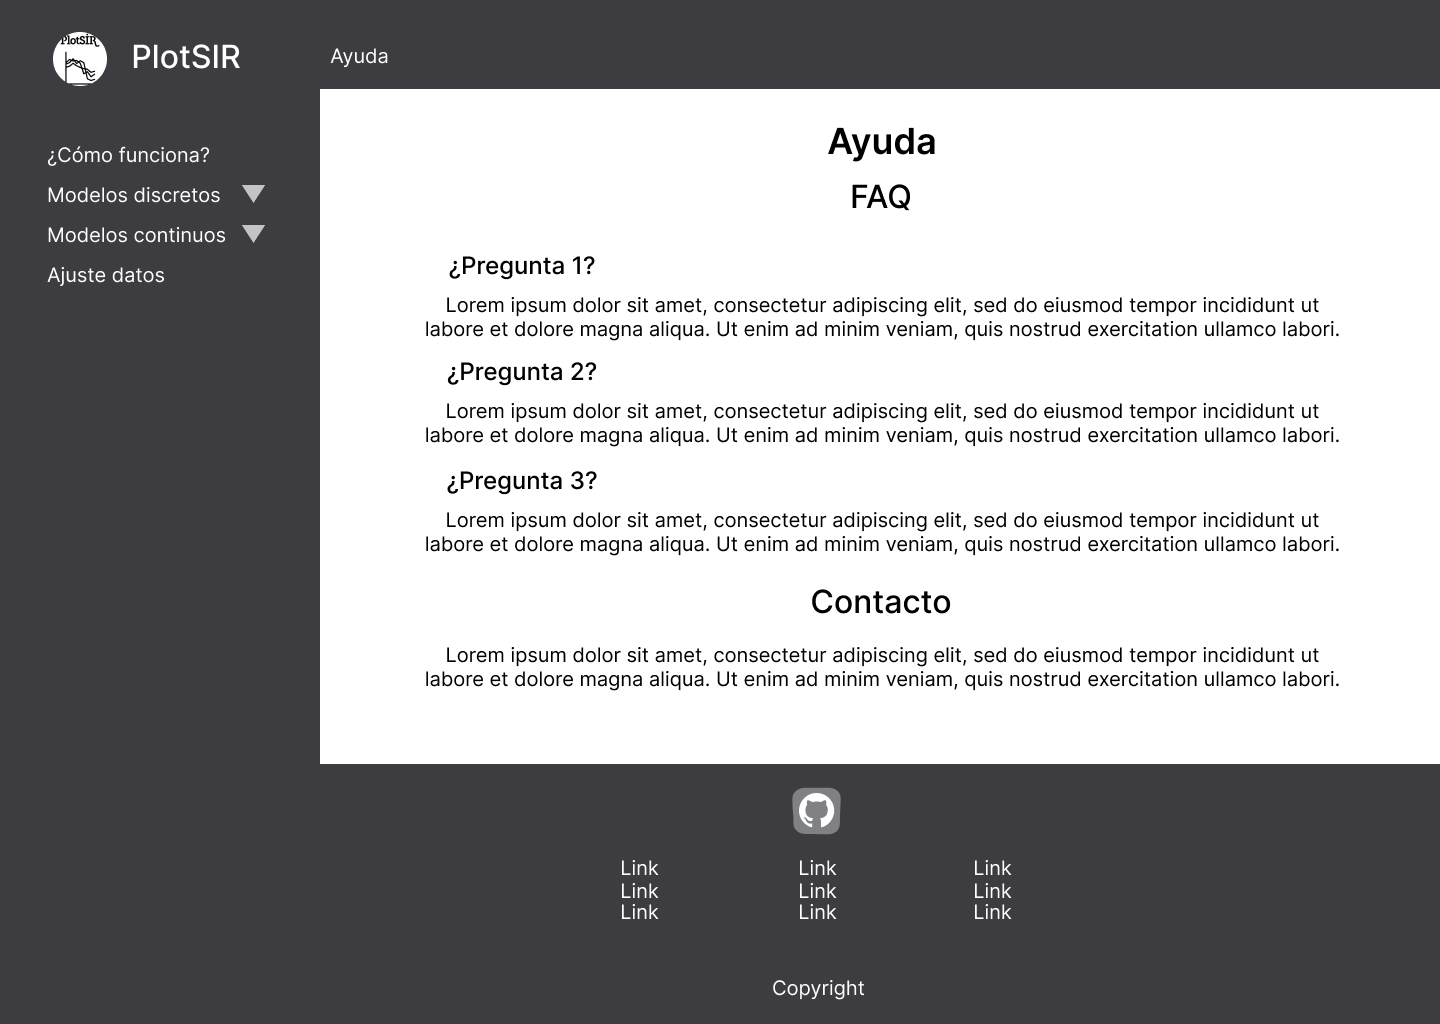
\includegraphics[scale=0.25]{Ayuda}
\end{center}
\end{figure}

\section{Manual de usuario}

\subsection{Descripción del proyecto}

El proyecto consiste en una página web de objetivo didáctico a la par que práctico, en la que se ofrece información sobre diversos modelos básicos de epidemiología de forma sencilla y clara a cualquier usuario.

De esta forma, el usuario puede aprender sobre varios modelos de epidemiología comprobando interactivamente el comportamiento de estos modelos en tiempo real, y cómo afectan los parámetros de cada uno de ellos a la evolución de los mismos.

Además, se pueden subir ficheros con datos, ya sean generados por el propio usuario o datos reales recogidos y comprobar el resultado de ajustar estos datos a los modelos mencionados, así como elegir el mejor modelo que ajusta a dichos datos.

Para acceder a la página web el usuario solo requiere de un dispositivo con un navegador de internet mediante el que acceder a la web, introduciendo la url correspondiente.

\subsection{Comenzando a usar la web}

Una vez introducida la url de la web en el navegador, aparecemos en la página principal de esta, la cual puede verse en \eqref{manual:home}.

\begin{figure}
\begin{center}
\caption{Página home o principal de la web.}
\label{manual: home}
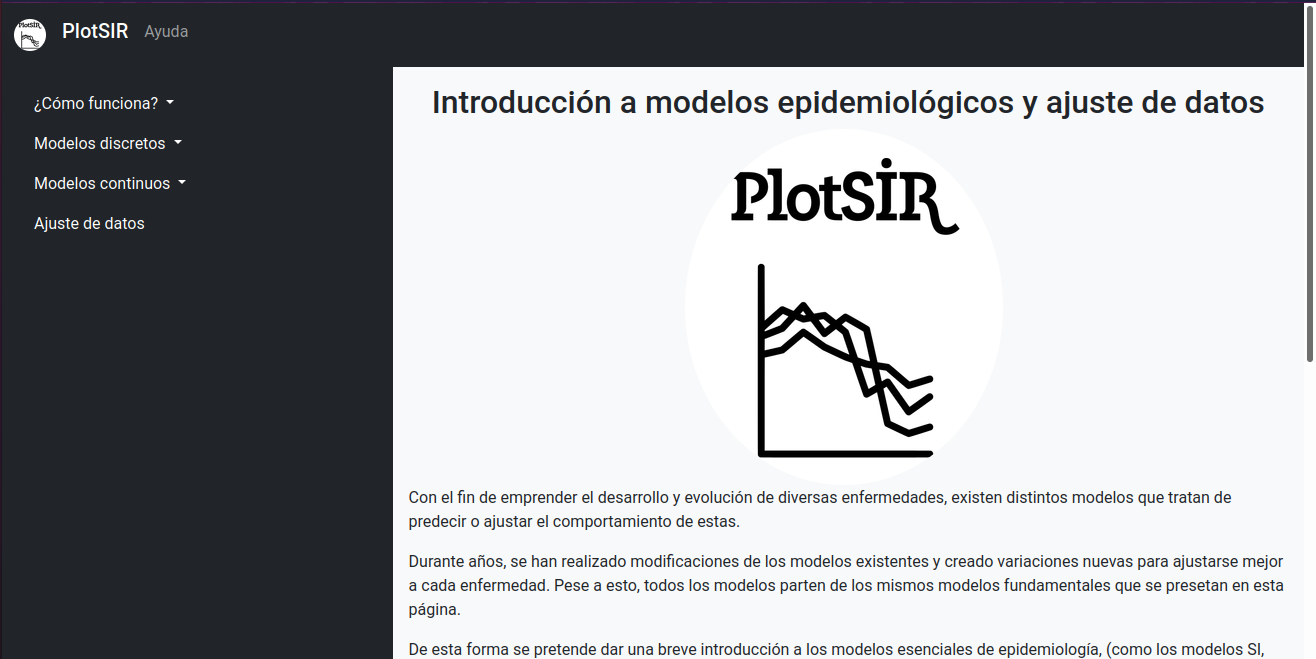
\includegraphics[scale=0.3]{pagina_home}
\end{center}
\end{figure}

Desde esta página podemos acceder a todas las funcionalidades e información de la web desde la barra de navegación y el menú lateral.

Además, la página principal es accesible en cualquier momento. Para volver a ella basta clicar en el logo de la esquina superior izquierda o el nombre de la página situado a su lado.

Asimismo, en la barra de navegación, situado al lado del título de la página encontramos el enlace a la ayuda de la misma. 

\subsection{Funcionalidades}

\subsubsection{Modificación de parámetros de los modelos interactivos}

\subsection{Ajuste de datos}

\subsection{Instalación del backend}





\section{Datos reales}

\textcolor{red}{Completar}





















% Part II
%\input{chapters/chapter5}

% ----------------------- %
% BIBLIOGRAFÍA
% ----------------------- %

% Estilo de cita.
%\usepackage{natbib} YA SE IMPORTA EN OTRO PUNTO, NO HACE FALTA PONERLO AQUI
% FUENTE CUSTOM
\bibliographystyle{apa-good}
% formato de citas original
%\bibliographystyle{unsrtnat}

%[citestyle=numeric]

% Añadimos la bibliografía al índice
\phantomsection
\addcontentsline{toc}{chapter}{Bibliografía}

\bibliography{bib/library}

\end{document}